%!TEX root = ../thesis.tex
%*******************************************************************************
%****************************** Fifth Chapter *********************************
%*******************************************************************************

\chapter{A comparative analysis to distinguish $\beta$-cell states and investigate shared transcriptional signatures across T2D-related stressors
}
\label{chp:meta_analysis}



% \begin{Abstract}

% \vspace{5mm}
% \label{abstract:chp3_meta_analysis}
% \hspace{-3mm}

% \textbf{\large Abstract} \\
    
% \end{Abstract}


\clearpage

\begin{Comment2}

\vspace{5mm}
\label{contr:chp3_meta_analysis}
\hspace{-3mm}

\textbf{\large Statement of Contributions} \\

\par This work was a joint effort with \textbf{Dr. Matthew Wortham}, Assistant Adjunct Professor at \href{https://ucsd.edu/}{University of California San Diego (UCSD)}.\\

\par Dr. Matthew Wortham generated most of the single-cell data utilized in this work. Additionally, experimental data was also generated by Dr. Chun Zeng, Dr. Ibrahim Omar and Dr. Han Zhu. All of the data was generated in the former group of Prof. Dr. Maike Sander az UCSD. Dr. Matthew Wortham and I identified additional, published studies to complement the in-house datasets for the building of the integrated reference and also for further dataset mapping analyses. I downloaded the raw sequencing data for the external studies.\\

\par I collected the raw sequencing data of all the studies and re-processed all single-cell data, performed quality control on all samples and conducted the preprocessing and all downstream analyses tasks on the data. I generated the figures pertaining to all analyses and these were adapted by Dr. Matthew Wortham. The interpretation of the results from the single-cell analysis was performed by Dr. Matthew Wortham and I.\\

\par The manuscript for the work presented in this study is currently being prepared and is headed by Dr. Matthew Wortham. My contribution in this scope is related to editing and proof-reading the manuscript, the generation of main and supplementary figures, the preparation of supplementary data and the compilation of all the code used during the course of the analysis.\\

\end{Comment2}

%
%\newpage\null\thispagestyle{empty}\newpage
%\clearpage

% \section{$\beta$-cell heterogeneity and adaptation in response to stress}

% In any given multicellular biological system, cellular heterogeneity  can arise from developmental programs establishing cellular subtypes, from changes in cellular state due to altered environments or cell-intrinsic fluctuations, and from stochastic variation in gene expression. Cellular heterogeneity has been shown to be involved in development, adaptation to dynamic environmental conditions, repair and regeneration, as well as disease.
% While it has long been apparent that not all $\beta$-cells in adult islets are identical, recent technological advances have shed further light on $\beta$-cell heterogeneity in terms of their morphology, identity and function. Although GSIS is the key function of mature $\beta$-cells, some $\beta$-cells may also retain non-secretory roles, necessary for overall islet function \textbf{\cite{liu_all_2017}}. This heterogeneity in $\beta$-cells is driven by topography and developmental origin \textbf{\cite{puri_plasticity_2015,roscioni_impact_2016}}, maturation state \textbf{\cite{salinno_-cell_2019}}, and stress response \textbf{\cite{xin_pseudotime_2018}}. Recent advances in characterization of $\beta$-cell heterogeneity have raised several important questions about the physiological significance of the prevalence of different $\beta$-cell sub-populations, , their role in diabetes pathogenesis, and the plasticity of individual $\beta$-cells.

% \subsection{Previously established $\beta$-cell heterogeneity}
% \colorbox{pink}{missing figure} \colorbox{green}{text clean-up} \colorbox{orange}{incomplete text} \\
% \subsubsection{Historical Perspective}
% In a study from 1960, Hellerström \textit{et. al.} identified regional differences in nuclear sizes and the position of nucleoli within the nuclei, depending on whether the $\beta$-cells were located centrally or peripherally in large or small islets in rat. The authors further suggested that these cytological differences could be interpreted as corresponding differences in functional states of $\beta$-cells, as lower activity in centrally located $\beta$-cells in large islets could be due to cells being older or due to lower concentrations of glucose and/or insulin, compared to the cells in the periphery or in small islets \textbf{\cite{hellerstrom_properties_1960}}. In 1986, Salomon and Meda demonstrated that $\beta$-cells in rat islets were heterogeneous in their ability to release insulin \textbf{\cite{salomon_heterogeneity_1986}}. In particular, the group of Daniel G. Pipeleers carried out pioneering work in characterizing and describing $\beta$-cell heterogeneity in rodents; they identified distinct $\beta$-cell sub-populations differing in glucose responsiveness, insulin secretion and NADPH levels \textbf{\cite{kiekens_differences_1992,schuit_glucose_1988,van_de_winkel_autofluorescence-activated_1983}}.

% \subsubsection{$\beta$-cell diversity: Insights from single-cell RNA sequencing (scRNA-seq)}
% The field of single-cell biology has revolutionized the characterization of cells and led to the identification of novel cell-types, cell states and a better understanding of mechanisms in health and diseases. This topic has been discussed in detail in \textbf{\hyperref[sec:scrna]{Section 1.5}}. Single-cell analyses have recapitulated the previously described idea concept of functional $\beta$-cell heterogeneity and \hl{....}  Another study identified that mature and immature and/or proliferative $\beta$-cells co-exist in healthy mouse islets. The immature $\beta$-cell cluster was characterized by downregulation of genes involved in insulin secretion, oxidative phosphorylation (OxPhos) and cell-cycle inhibition, as well as upregulation of genes involved in \textit{cAMP} and \textit{WNT} signaling. Further, trajectory inference %(see \hyperref[sec:sc_tpi]{TI methods}) 
% suggested a continuum of transition between the immature and mature states, rather than discrete phenotypes \textbf{\cite{sachs_targeted_2020}}. In another study employing mouse models, the authors defined $\beta$-cell maturity using arbitrarily defined levels of \textit{Pdx1} and \textit{Mafa}, and showed that adult islets are composed of mature (\textit{Pdx1}\textsuperscript{\textit{high}} \textit{Mafa}\textsuperscript{\textit{high}}) and immature (\textit{Pdx1}\textsuperscript{\textit{low}} \textit{Mafa}\textsuperscript{\textit{low}}) $\beta$-cells and the balanced proportion of these sub-populations might contribute to proper islet function and insulin release \textbf{\cite{nasteska_pdx1low_2021}}. Another study demonstrated the adaptive plasticity of $\beta$-cells to reversible chronic ER stress wherein $\beta$-cells undergo a reprogramming of their transcriptome and proteome. More than half of the genes involved in ER protein processing as well as markers of $\beta$-cell identity were compromised due to chronic stress whereas upon alleviation, $\beta$-cells regained their mature identity. The authors postulated that the heterogeneity in the maturity of $\beta$-cells in the islets might be a physiological response to cycles of ER stress and recovery in vivo \textbf{\cite{chen_adaptation_2022}}.\\\\
% With recent advances in the throughput of single-cell experiments, accumulating single-cell data and multiple scRNA-seq data analysis and integration approaches, large reference atlases, which comprise of millions of cells across several tissues, organs, developmental stages and/or conditions are now routinely generated \textbf{\cite{regev_human_nodate}}. These atlases help understand cellular heterogeneity, and provide an opportunity to learn from several single-cell datasets simultaneously, allowing for automatic annotation of new datasets and easy comparative analyses across several conditions \textbf{\cite{rood_impact_,lotfollahi_mapping_2021}}. The integrated \gls{mia} by Hrovatin \textit{et. al.} \textbf{\cite{hrovatin_delineating_2023}}, represents a comprehensive scRNA-seq atlas of mouse pancreatic islets, integrating over 300,000 cells across multiple developmental stages and disease conditions. The study also provided insights into the heterogeneity and dynamic states of $\beta$-cells during development, aging, and under diabetic conditions and revealed an intermediate $\beta$-cell state between healthy controls and the different diabetes models, depicted heterogeneous expression of known $\beta$-cell maturity and dysfunction markers across $\beta$-cell states and described pathways indicative of the different  $\beta$-cell dysfunction phenotypes. Overall, the \gls{mia} complemented the growing body of research on islet $\beta$-cell biology and highlighted the critical role of high-resolution single-cell atlases. 

% \subsection{$\beta$-cell adaptation and response to stress}
% \colorbox{pink}{missing figure} \colorbox{yellow}{missing text} \\

% The pathogenesis of \gls{t2d} is intricately linked to the dynamic response of $\beta$-cells to insulin resistance, wherein increased insulin demand is met by compensatory increases of insulin release, in order to maintain blood glucose homeostasis. It is evident from rodent studies that, both, expansion of $\beta$-cell mass and enhanced $\beta$-cell function are important for $\beta$-cell compensation. 


% The failure of $\beta$-cells to compensate for insulin resistance results in overt diabetes. $\beta$-cell dysfunction is characterized by loss of identity and lack of function.\\\\
% A central component of $\beta$-cell dysfunction in \gls{t2d} is the loss of functional mature identity and return to a progenitor-like state, termed as `dedifferentiation'. The dedifferentiation process is attributed to several factors such as oxidative stress, gluco- and lipo-toxicity, pro-inflammatory cytokines and altered gene expression.\\
% In particular, using PAGA, Hrovatin et. al further deciphered the relationship between healthy and diseased states by identifying a shared intermediate state prior to the T1D or T2D model state. Further examination of this intermediate state revealed differences in expression of most of the shared diabetes DEGs between healthy and intermediate states and further changed in the diabetic states. Based on these observations, the authors concluded that the intermediate state could represent a snapshot of the progression of $\beta$-cell dysfunction during diabetes. 


% %Based on clinical observations and work with animal models of diabetes, Weir \& Bonner-Weir proposed five stages of $\beta$-cell dysfunction during diabetes progression \textbf{\cite{weir_five_2004}}. The stages describe changes in $\beta$-cell mass, phenotype and function, ranging from initial compensation (Stage-1) with increased insulin secretion and intact $\beta$-cell function, through adaptation (Stage-2) and early decompensation (Stage-3) characterized by rising glucose levels and $\beta$-cell de-differentiation, to stable (Stage-4) and severe (Stage-5) decompensation marked by significant loss of $\beta$-cell mass and function. 


% % Failure of $\beta$-cell compensation is the defining event during the progression of \gls{t2d}. 

\clearpage

\section{Introduction}
\label{sec:chp3_intro}
\par There exists a complex landscape of $\beta$-cell heterogeneity where not all $\beta$-cells are uniform but vary widely in morphology, function and gene expression. With the advent of single-cell technologies, researchers have explored this variation more precisely and identified $\beta$-cell sub-populations ranging from healthy and fully functional states to stressed and dedifferentiated states. A cell state is an essential facet of cellular identity and gene expression changes associated with cellular states may be seen during various physiological processes \textbf{\cite{morris_evolving_2019,zeng_what_2022}}. Single-cell techniques allow us to monitor these transcriptional state changes during adaptation or failure with single-cell precision. This heterogeneity is pivotal for the adaptive responses by $\beta$-cells such as enhanced \acrfull{gsis} and $\beta$-cell proliferation, which are essential for maintaining adequate $\beta$-cell mass and function in face of metabolic challenges. However, significant gaps remain in our understanding, particularly regarding how chronic metabolic stress triggers transitions from a state of compensatory responses to $\beta$-cell dysfunction, which is the critical determinant for \gls{t2d}.\\ 
%Studying the differences between functional, mature and dysfunction-associated immature states could potentially inform future diabetic therapies.\\

\par The topic of $\beta$-cell heterogeneity, dysfunction and failure has been extensively studied with \acrfull{scr} employing mouse models, as they provide predictable disease progression. However, findings from individual studies are difficult to relate to each other, and there is lack of consensus on how many $\beta$-cell sub-populations exist or why $\beta$-cells fail \textbf{\cite{liu_all_2017,miranda_pancreatic_2021}}. This could be attributed to factors ranging from biological variability such as heterogeneous cellular states, use of different stressors to induce dysfunction to technical variations like study-specific batch effects or other unknown confounding variables. To circumvent this, several \gls{scr} data analysis and integration approaches are available that enable the creation of integrated atlases that represent a curated resource allowing for direct comparison of multiple studies simultaneously \textbf{\cite{luecken_benchmarking_2021}}. Such atlases have become invaluable in providing insights beyond individual datasets.\\

\par In this chapter, we performed a meta-analysis of seven \gls{scr} islet studies and present an integrated landscape of islet $\beta$-cells across various models of adaptation and decompensation. We performed a comprehensive analysis of the heterogeneous $\beta$-cell subsets across all the datasets and identified unique and shared transcriptional profiles of $\beta$-cells across the studies. Furthermore, we also explored \glspl{grn} underlying the transcriptional heterogeneity of $\beta$-cells and identified identified key \gls{tf}-target gene `regulons` that govern $\beta$-cell function and adaptation under different physiological conditions. We also demonstrated a practical application by applying the findings to additional \gls{scr} studies. Together, our meta-analysis offers critical insights into the dynamics of $\beta$-cell adaptation and failure, providing a valuable resource for future studies aiming to decipher the molecular mechanisms driving \gls{t2d} progression and potential therapeutic interventions.

%\clearpage
% \subsection{Previously established $\beta$-cell heterogeneity}
% \label{subsec:trial}


\section[An integrated atlas of pancreatic islet $\beta$-cells across various models of $\beta$-cell adaptation and decompensation]{An integrated atlas of pancreatic islet $\beta$-cells across\\various models of $\beta$-cell adaptation and decompensation}
\label{sec:int_atlas}

\begin{figure}[b!]
\centering
% \vspace{-15pt}
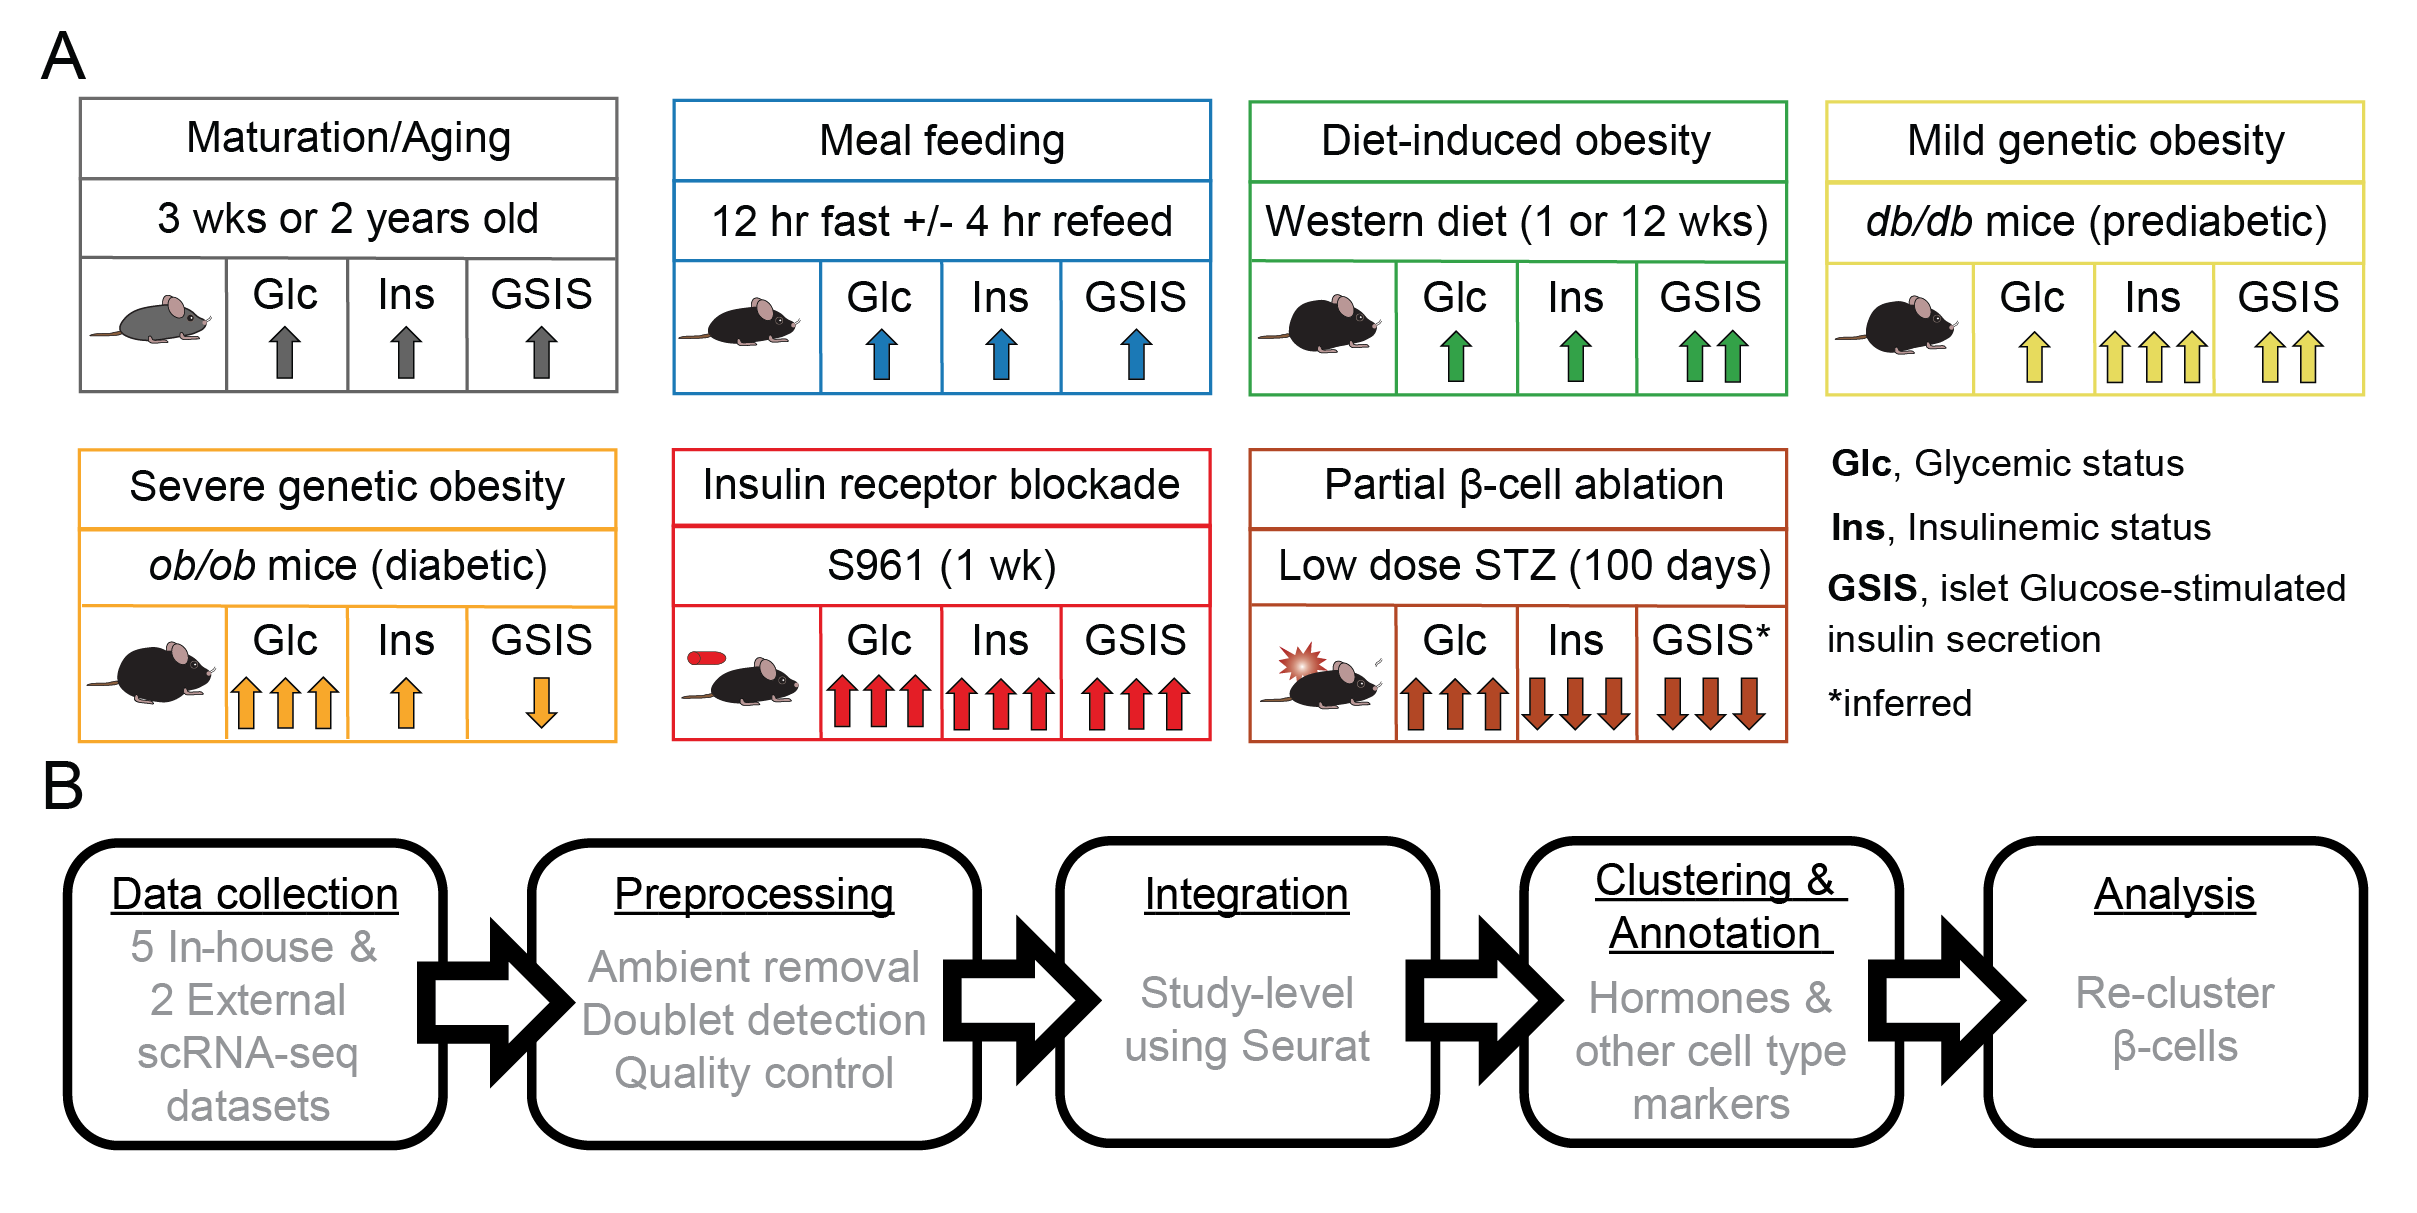
\includegraphics[width=\linewidth]{Chapter5/Fig/F3-1-v2-02.png}
\caption[Workflow to build an integrated atlas to study $\beta$-cell transcriptome]{\textbf{Workflow to build an integrated atlas to study $\beta$-cell transcriptome.} \textbf{(A)} Overview of the various $\beta$-cell workload models used in this study. For every model, the effect of the workload on the glycemic, insulinemic and \gls{gsis} status of the animals is indicated. The orientation of the arrows indicate the directionality of the response while the number of arrows indicate the intensity. \textbf{(B)} Schematic depicting the workflow for preprocessing, integration, clustering and annotation, and further downstream analysis on all $\beta$-cells}
\label{fig:chp3_workflow}
\end{figure}

\par To better understand the mechanisms underlying successful and failed $\beta$-cell compensatory responses, we integrated seven \gls{scr} datasets spanning a broad range of $\beta$-cell workload, defined as insulin demand per $\beta$-cell \textbf{(\autoref{fig:chp3_workflow} A; \autoref{tab:app_chp3_study};} see \hyperref[subsubsec:met_chp3_data]{\textbf{Methods}}\textbf{)}. We included five datasets generated in-house and further incorporated two previously published datasets to include additional hyperglycemic models: islets from older \textit{ob/ob} animals (severe genetic obesity) and islets from mice subjected to partial $\beta$-cell ablation by \gls{stz}, (partial $\beta$-cell ablation) \textbf{(\autoref{fig:chp3_workflow} A)} \textbf{\cite{chung_endocrine-exocrine_2020,sachs_targeted_2020}}. The samples across the seven datasets varied by age and strain \textbf{(\autoref{tab:app_chp3_study})}. An additional study incorporating islets from 3-week-old or 2-year-old mice (maturation/aging) was used as a reference point for developmental maturity \textbf{(\autoref{fig:chp3_workflow} A)}. The same study, along with the data from diet-induced obesity model were also utilized for the comprehensive analysis of islet-associated immune cells in \textbf{\autoref{chp:diet_aging}} \textbf{(\autoref{fig:chp3_workflow} A)}. Out of the seven studies, six of them isolated islets exclusively from male mice, whereas the meal feeding dataset pooled islets from both male and female mice \textbf{(\autoref{fig:chp3_workflow} A; \autoref{tab:app_chp3_study})}. Complementing the \textit{ob/ob} model, we included single-cell data obtained from a prediabetic \textit{db/db} mouse model (mild genetic obesity) \textbf{(\autoref{fig:chp3_workflow} A)}. This study included islets isolated from 6-week-old and 9-week-old \textit{db/db} mice and their corresponding lean (\textit{db/+}) controls. Finally, we incorporated a severely hyperglycemic model which involved the use of insulin receptor antagonist S961 to increase $\beta$-cell workload without ablating $\beta$-cells (insulin receptor blockade) \textbf{(\autoref{fig:chp3_workflow} A)} \textbf{\cite{wortham_metabolic_2024}}. We applied the same preprocessing steps with sample-specific thresholds in order to perform \gls{qc} and exclude cells with low quality metrics \textbf{(}see \hyperref[subsubsec:met_chp3_preprocessing]{\textbf{Methods}}\textbf{)}. To enable joint analysis and comparisons of the datasets, we performed data integration in order to create a joint embedding space \textbf{(\autoref{fig:chp3_workflow} B;} see \hyperref[subsubsec:met_chp3_integration]{\textbf{Methods}}\textbf{)}. Integration of these seven datasets allowed us to account for the various batch-effects arising from sample handling, housing conditions, and mouse strains used.\\



% \begin{figure}[H] The inclusion of these two early time-points \hl{...}
% \centering
% 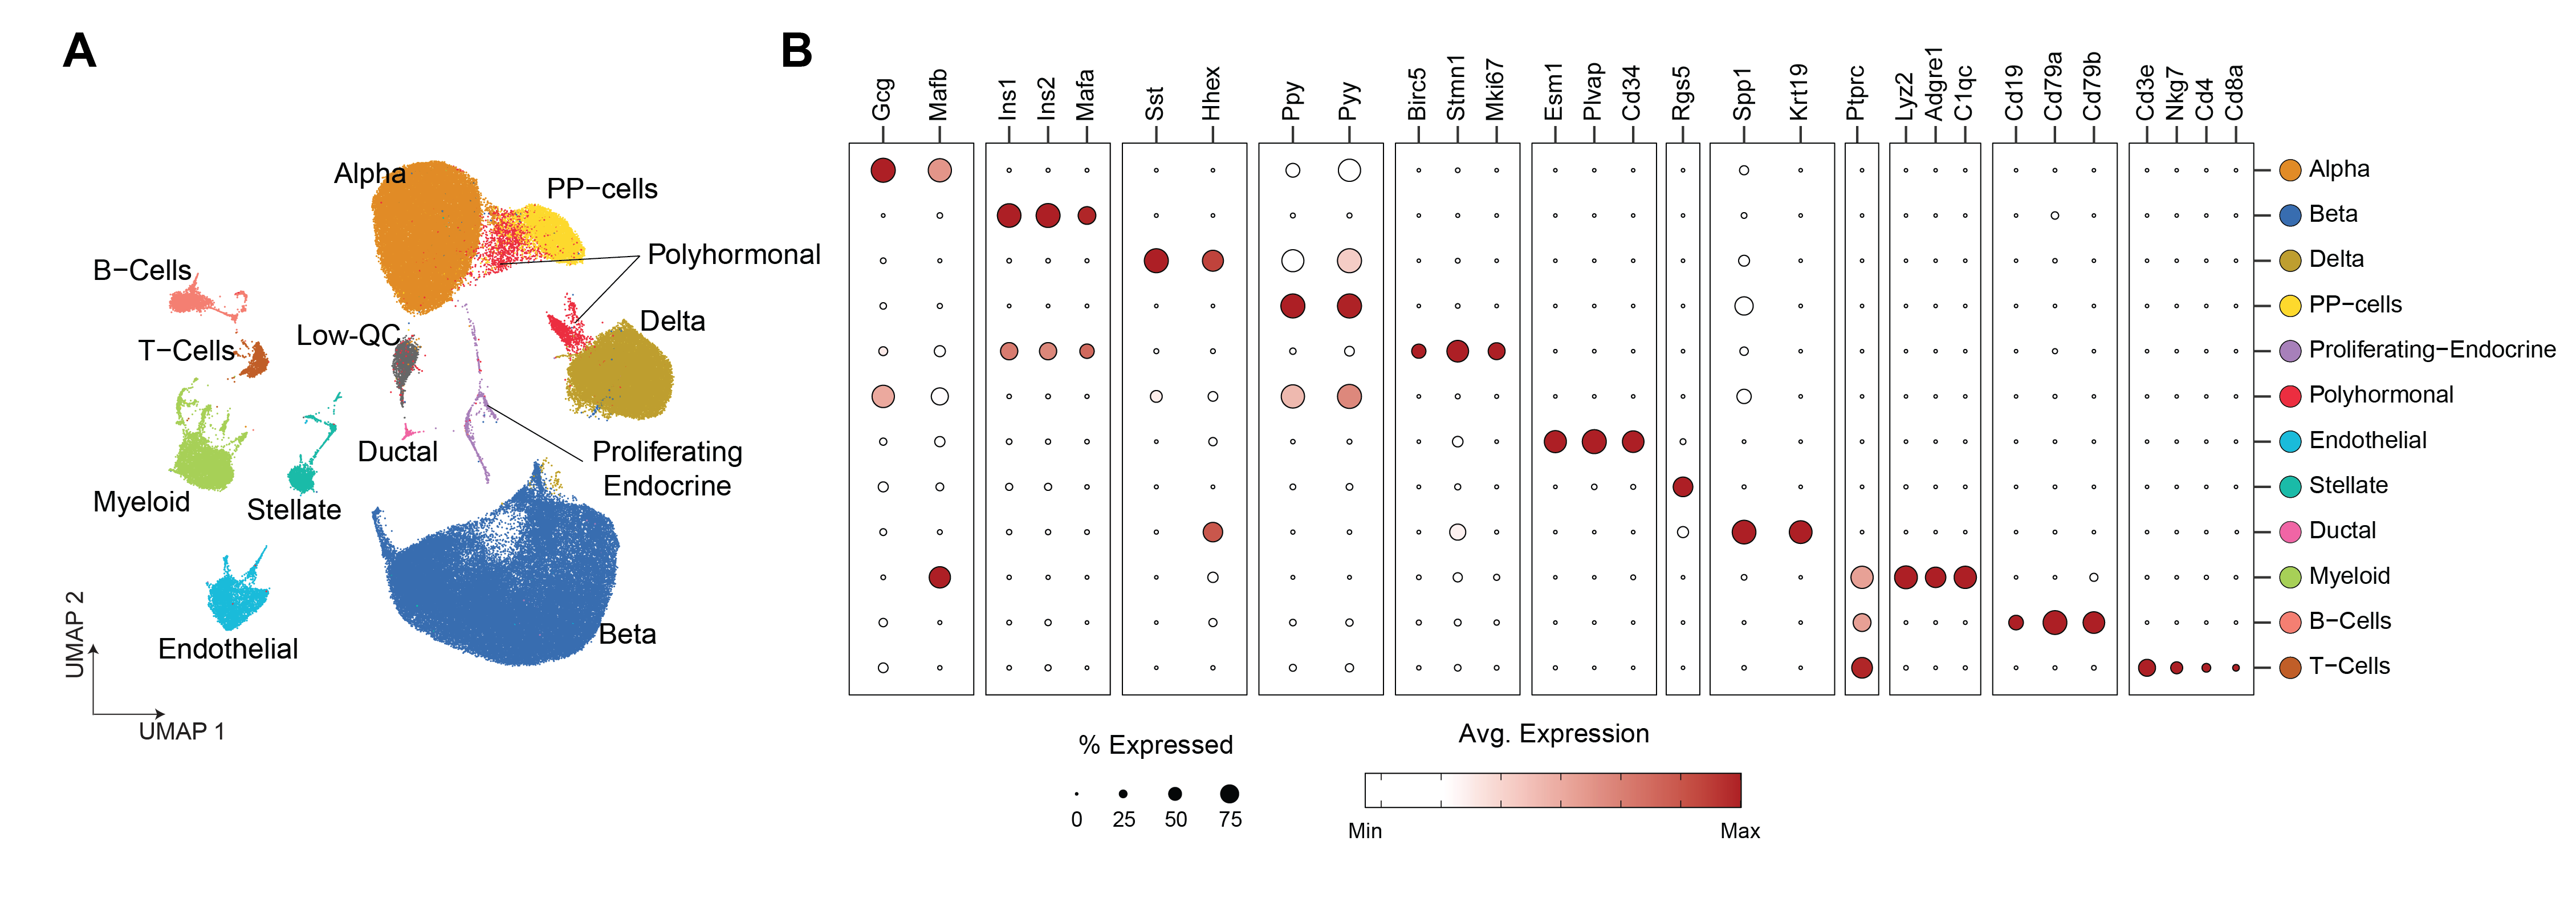
\includegraphics[width=\linewidth]{Chapter5/Fig/F3-2-01.png}
% \caption[fig3-2]{\textbf{Integrated dataset of seven scRNA-seq studies across several models of $\beta$-cell decompensation and hyperglycemia.}\\
% \textbf{(A)} UMAP embedding of the integrated dataset depicting celltype annotations based on the expression of known markers. \textbf{(B)} UMAP embedding of the integrated dataset depicting the seven scRNA-seq studies. Datasets are described in Supplementary Table \ref{tab3-1}. \textbf{(C)} Number of cells per sample within each study. \textbf{(D)} Dotplot depicting hallmark markers for the annotated celltypes in panel \textbf{A}. \textbf{E} Number of cells per celltype.}
% \label{fig:3-2}
% \end{figure}
% \clearpage


% \captionof{figure}{\textbf{Integrated dataset of seven scRNA-seq studies across several models of $\beta$-cell decompensation and hyperglycemia.} \textbf{(A)} UMAP embedding of the integrated dataset depicting celltype annotations based on the expression of known markers. \textbf{(B)} UMAP embedding of the integrated dataset depicting the seven scRNA-seq studies. Datasets are described in Supplementary Table \ref{tab3-1}. \textbf{(C)} Number of cells per sample within each study. \textbf{(D)} Dotplot depicting hallmark markers for the annotated celltypes in panel \textbf{A}. \textbf{E} Number of cells per celltype.}


\begin{figure}[b!]
\centering
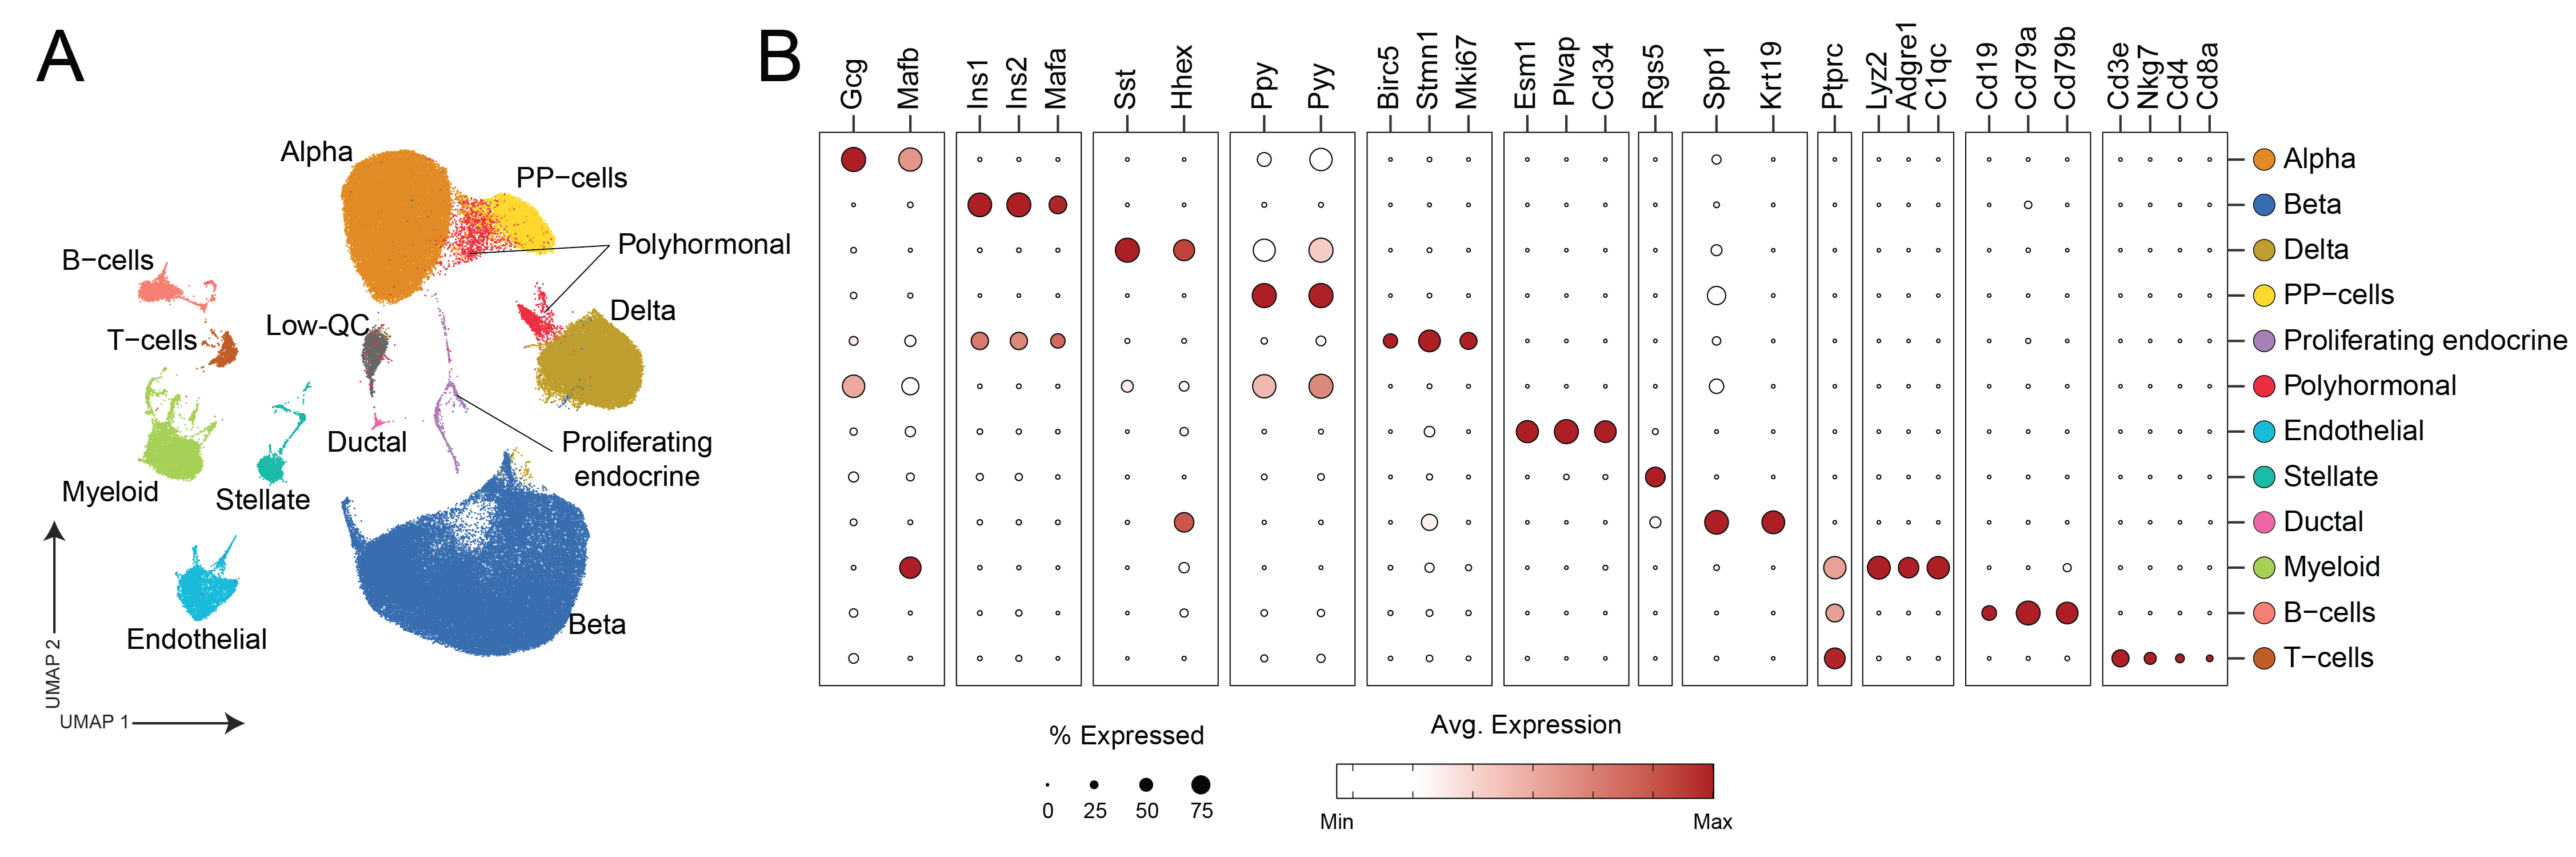
\includegraphics[width=\linewidth]{Chapter5/Fig/F3-2-v2-01.png}
\caption[Integrated atlas of seven \glsentryshort{scr} studies]{\textbf{Integrated atlas of seven \gls{scr} studies.} \textbf{(A)} \gls{umap} embedding of the integrated dataset depicting the various cell types identified on the basis of the expression of known markers. \textbf{(B)} Dot plot depicting hallmark marker genes for all annotated cell types in \textbf{(A)}. The color of the dots represent the scaled average expression of the genes and the size of the dots correspond to the percentage of cells expressing the gene.}
\label{fig:chp3_fulldata}
\end{figure}

%\clearpage

\par The integrated embedding space showed clear separation into distinct clusters, which corresponded to distinct cell types that originated from the different datasets \textbf{(\autoref{fig:chp3_fulldata} A)}. This provided empirical evidence that data integration was indeed successful, ensuring optimal trade-off between batch correction and biological conservation on the level of cell types \textbf{(\autoref{fig:app_chp3_study} A)}. The integrated dataset contained 124,191 cells across 16 samples \textbf{(\autoref{fig:app_chp3_study} B; \autoref{tab:app_chp3_cellnumbers})}. We manually annotated the four major islet cell types using the expression of hormone markers: Alpha ($\alpha$) – \textit{Gcg}, Beta ($\beta$) - \textit{Ins1} and \textit{Ins2}, Delta ($\delta$) – \textit{Sst} and PP-cells ($\gamma$) – \textit{Ppy} \textbf{(\autoref{fig:chp3_fulldata} B)}. Apart from the major hormone secreting cell types, we also annotated polyhormonal cells expressing more than one hormone marker simultaneously. We identified the polyhormonal cells with a step-wise strategy of: \textbf{(i)} setting thresholds of hormone expression to define the four endocrine cell types, \textbf{(ii)} identifying cells co-expressing any of the two hormone markers and \textbf{(iii)} referring to existing literature about polyhormonal singlets and polyhormonal doublets \textbf{\cite{sachs_targeted_2020, perez-frances_pancreatic_2021}}. Based on this, we excluded Alpha-Beta and Beta-Delta cells as probable polyhormonal doublets from further analysis. The remaining polyhormonal cells were identified as Alpha-PP (\textit{Gcg - Ppy}) and Delta-PP (\textit{Sst - Ppy} \textbf{(\autoref{fig:chp3_fulldata} A,B)}. Additionally, we also annotated non-endocrine cell types such as endothelial – \textit{Pecam1}, immune cell types such as myeloid – \textit{Lyz2, Adgre1}, B-cells - \textit{Cd19} and T-cells - \textit{Cd3e}, stellate – \textit{Rgs5} and ductal – \textit{Krt19} \textbf{(\autoref{fig:chp3_fulldata} B)}.

%\clearpage

\section[Clustering of pseudobulk $\beta$-cells segregates hyperglycemic from normoglycemic samples]{Clustering of pseudobulk $\beta$-cells segregates hyper-\\glycemic from normoglycemic samples}
\label{sec:chp3_pseudobulk}

\par To focus upon transcriptional changes in islet $\beta$-cells during compensation and failure, we sub-clustered the $\beta$-cells for further analysis. We extracted cells annotated as Beta and Proliferating endocrine and performed additional \gls{qc} to remove polyhormonal cells that expressed non-$\beta$-cell hormones (\textit{Gcg, Sst, Ppy}). From the cells annotated as Proliferating endocrine, we retained only the proliferating $\beta$-cells. We re-integrated these $\beta$-cells across the seven studies in a similar manner to the full integrated dataset \textbf{(\autoref{fig:chp3_pseudobulk} A; \autoref{tab:app_chp3_cellnumbers};} see \hyperref[subsubsec:met_chp3_betareint]{\textbf{Methods}}\textbf{)}. The re-integration of $\beta$-cells was necessary to account for any nested batch effects that might have been persistent across the studies. On the integrated embedding, the $\beta$-cells from the healthy controls across the six studies and the 2-year-old mice from maturation/aging study overlapped with each other, whereas the cells from the experimental samples in the six studies and the 3-week-old mice mapped away from the control groups \textbf{(\autoref{fig:app_chp3_betastudy})}.\\

\begin{figure}[t!]
\centering
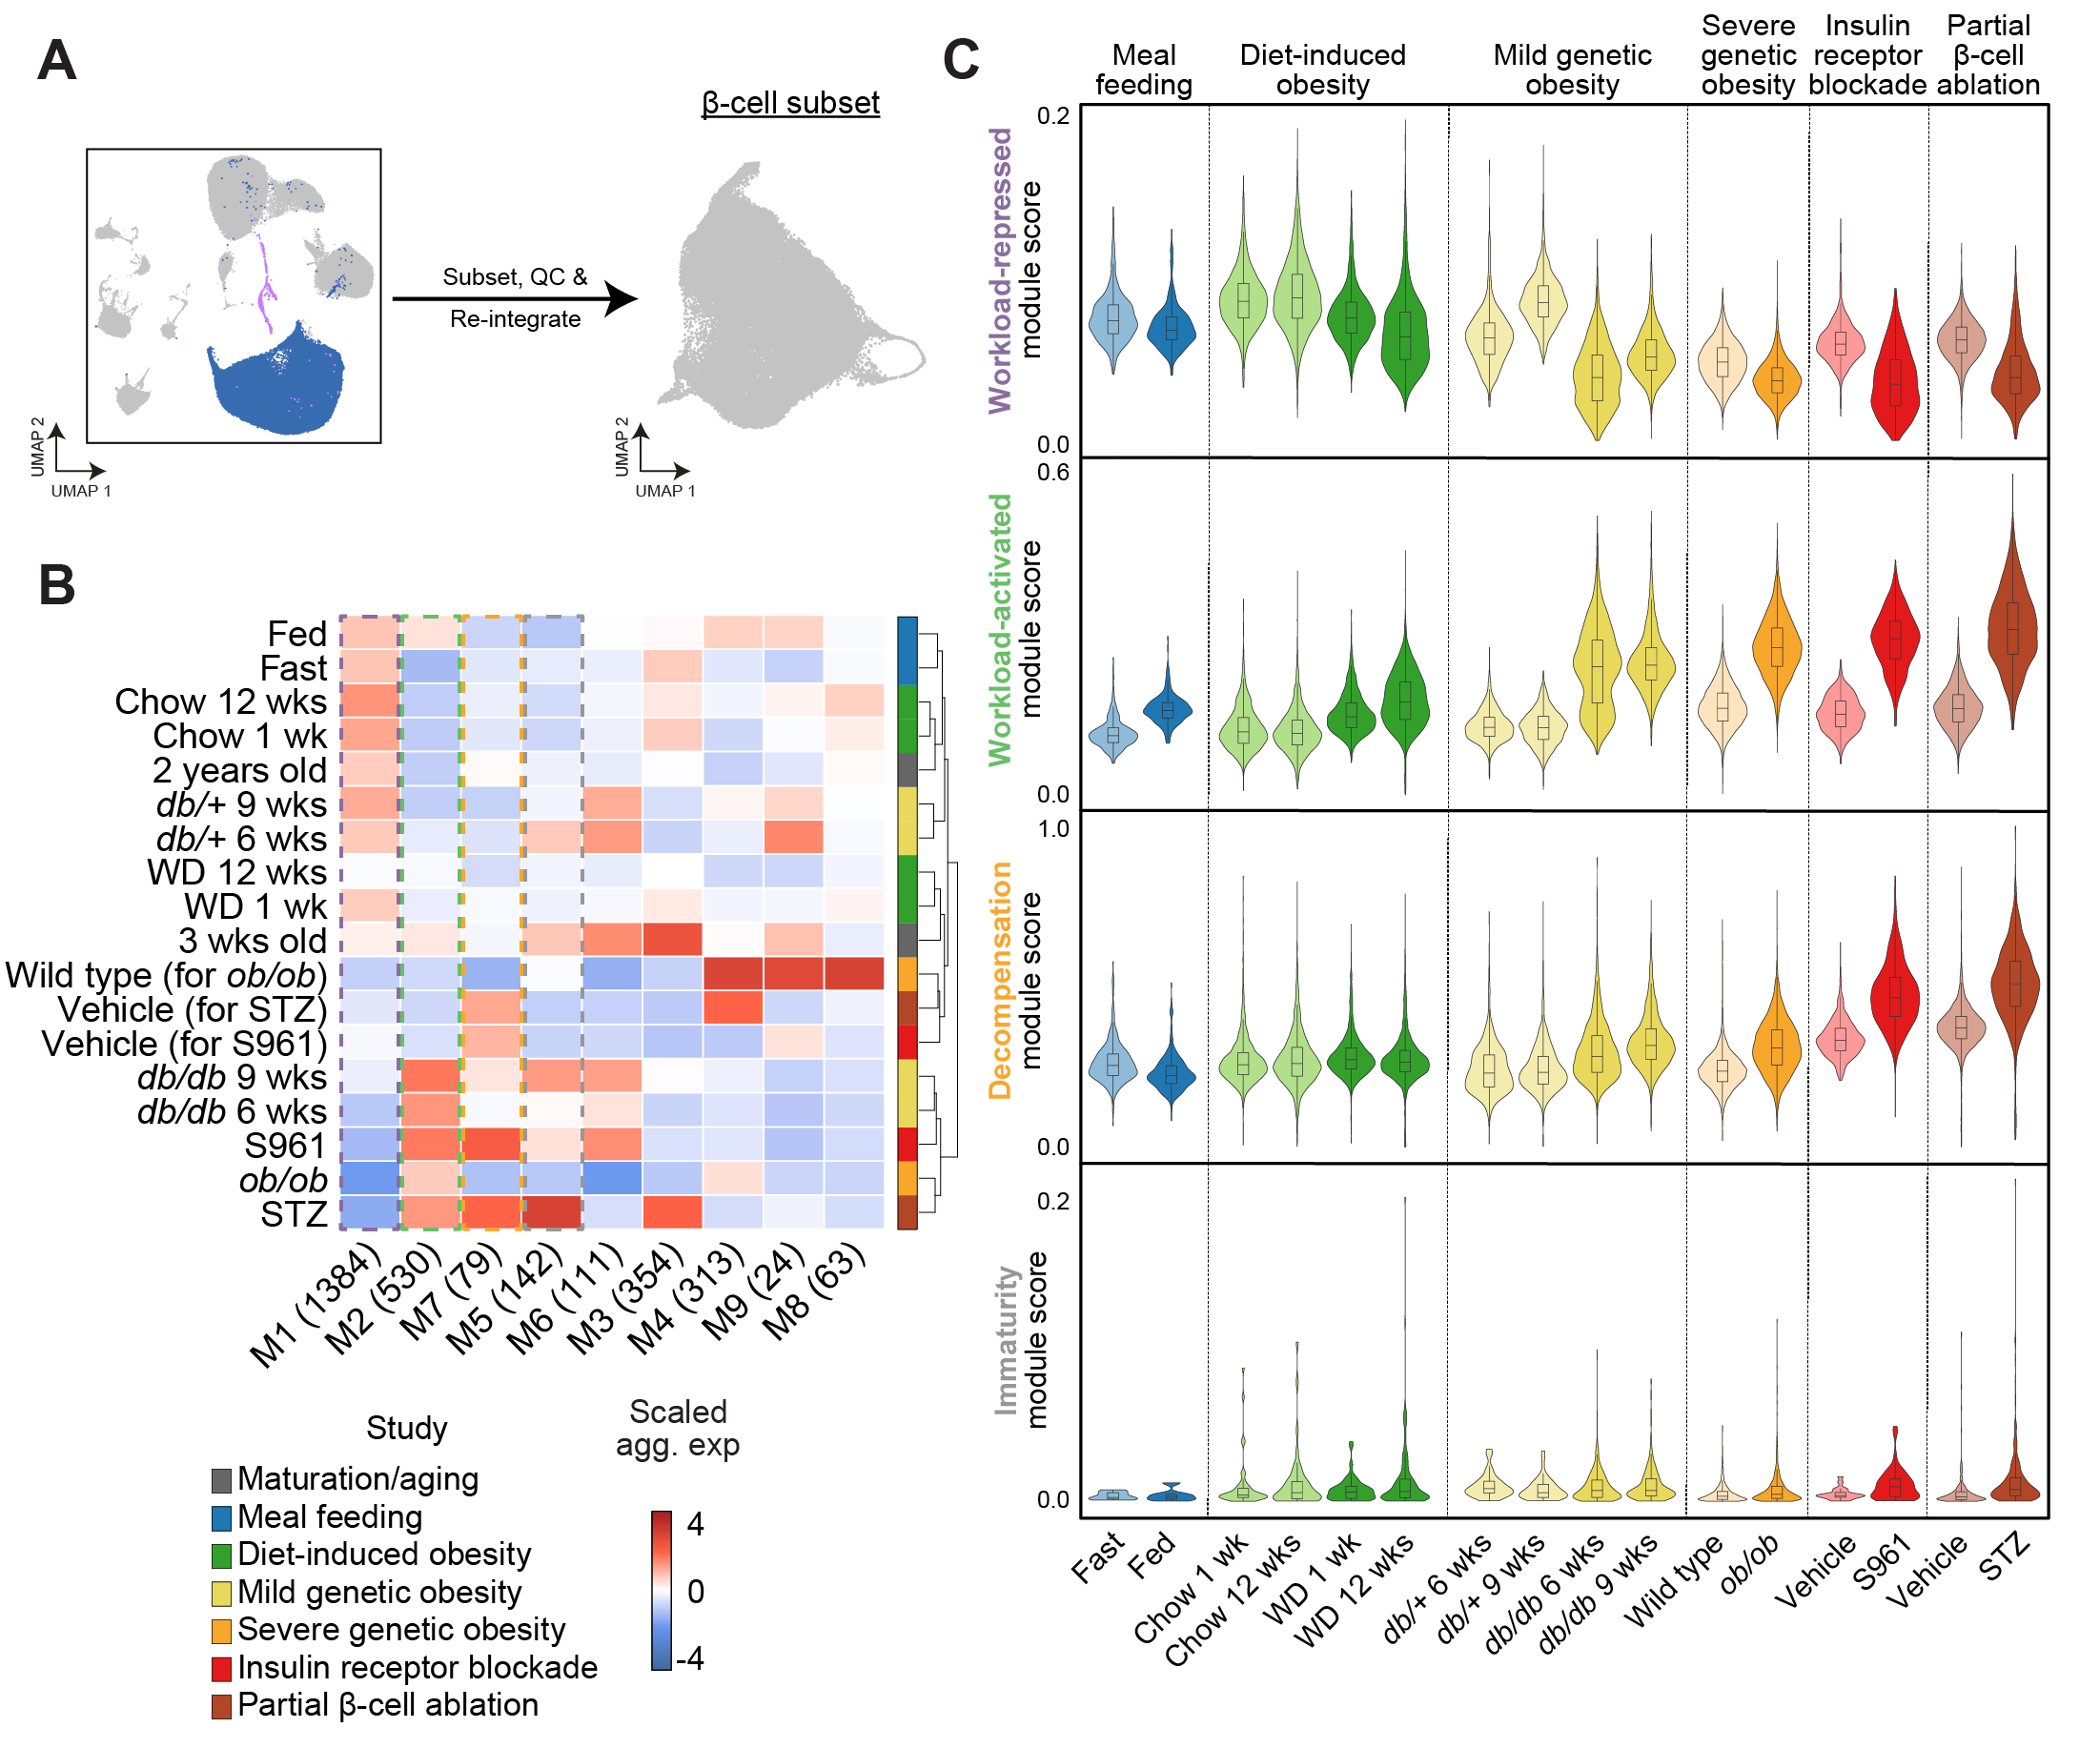
\includegraphics[width=\linewidth]{Chapter5/Fig/F3-3-01.png}
\caption[Hierarchical clustering of pseudobulk $\beta$-cells across all samples]{\textbf{Hierarchical Clustering of pseudobulk $\beta$-cells across all samples.} \textbf{(A)} Schematic depicting the workflow to obtain a  $\beta$-cell specific subset from the full integrated data. On the left, the \gls{umap} embedding of the full integrated data is shown with $\beta$-cells and Proliferating Endocrine cells highlighted. On the right, the \gls{umap} embedding of the re-integrated $\beta$-cell specific subset is shown. \textbf{(B)} Heatmap depicting the hierarchical clustering of samples from seven studies based on the scaled aggregate expression of 3000 \glspl{hvf} across pseudobulk $\beta$-cells. The number of genes in each of the module is indicated in parantheses. \textbf{(C)} Violin plots depicting gene set score of four modules highlighted in (\textbf{B}) across six studies for all $\beta$-cells. The maturation/aging study is not depicted. On the overlay box plots, the middle horizontal line represents the median, the box represents the inter-quartile range and the whiskers represent the minimum and maximum values. The number of cells are indicated in \textbf{\autoref{tab:app_chp3_cellnumbers}}.}
\label{fig:chp3_pseudobulk}
\vspace{-10pt}
\end{figure}

\par To provide a stringent assessment of the effectiveness of the re-integration and to test whether the re-integration of $\beta$-cells was adequate for downstream analyses, we performed hierarchical clustering of all samples based on the expression profiles of pseudobulk $\beta$-cells. We aggregated the normalized expression values of the 3000 \glspl{hvf} across all the experimental samples and the aggregated expression matrix was used to cluster genes into nine modules, grouping genes with similar expression profiles across the samples \textbf{(\autoref{fig:chp3_pseudobulk} B;} see \hyperref[subsubsec:met_chp3_pseudo]{\textbf{Methods}}\textbf{)}. Based on these gene modules, hierarchical clustering of the experimental samples separated the hyperglycemic models such as the insulin receptor blockade with S961, obese \textit{ob/ob} animals and partial $\beta$-cell ablation model from their normoglycemic controls. However, these normal controls did not cluster with the other healthy controls of the remaining studies, likely due to enduring batch effects between the studies. The 6-week-old and the 9-week-old \textit{db/+} animals clustered together and away from the \textit{db/db} cohorts that also clustered together. Similarly, samples with mice fed chow diet for 1 or 12 weeks clustered together and away from the \gls{wd}-fed counterparts. Interestingly, the fasting and feeding samples from the meal feeding study clustered together \textbf{(\autoref{fig:chp3_pseudobulk} B)}, possibly reflecting the minimal effect of the feeding intervention on $\beta$-cell workload compared to other models that exert higher workloads.\\

%\clearpage
\par We then performed gene set scoring on a single-cell level for three modules (\textit{Modules M1,M2} and \textit{M7}) identified from the hierarchical clustering of pseudobulk $\beta$-cells \textbf{(\autoref{fig:chp3_pseudobulk} C;} see \hyperref[subsubsec:met_chp3_scoring]{\textbf{Methods}}\textbf{)}. Module \textit{M1} was repressed by all conditions of increased workload and contained known markers of $\beta$-cell function (\textit{Mafa, Slc2a2}) and development (\textit{Neurod1, Pdx1}) as well as ion homeostasis (\textit{Atp2a2, Trpm5}) and was termed as workload-repressed module \textbf{(\autoref{fig:chp3_pseudobulk} C,} top row\textbf{)}. On the other hand, module \textit{M2} was activated in response to increased $\beta$-cell workload in models of mild (\textit{db/db}) and severe (\textit{ob/ob}) genetic obesity, insulin receptor blockade (S961) and partial $\beta$-cell ablation (\gls{stz}). The expression of this module was also slightly elevated in response to feeding as well as in the young 3-week-old mice. The module \textit{M2} was also associated with genes involved in protein processing in \gls{er} (\textit{Calr, Dnajb11, Hspa5}) and translation (\textit{Sec11a/c, Spcs1/2}). Therefore, we termed this module as workload-activated module \textbf{(\autoref{fig:chp3_pseudobulk} C,} middle row\textbf{)}. Additionally, this analysis also revealed a decompensatory profile (module \textit{M7}), which characterized the insulin receptor blockade as well as the partial $\beta$-cell ablation models (S961+\gls{stz}) \textbf{(\autoref{fig:chp3_pseudobulk} C,} bottom row\textbf{)}. This module was comprised of several ribosomal genes (\textit{Rpl\textsuperscript{*}} and \textit{Rps\textsuperscript{*}}) which were up-regulated by $\beta$-cells. Interestingly, we also identified the expression of genes involved in \glslink{dna}{DNA} replication and cell division (\textit{Stmn1, Top2a, Mki67}) in module M7, indicating that these $\beta$-cells are proliferating which well-documented to occur in response to increased workload.\\

%We also identified \gls{stz}-specific module \textit{M5}, which is likely resembles the m\gls{stz}-specific  GP8 and GP23 identified in \gls{mia} and was associated with immaturity \textbf{(\autoref{fig:chp3_pseudobulk} C,} bottom row\textbf{)} In the \gls{mia} \textbf{\cite{hrovatin_delineating_2023}}, the authors identified thathree gene programs (GPs): GP2, GP3 and GP4 which showed higher activity in the \textit{db/db + mSTZ} state and contained known diabetes markers or were associated with \glslink{er}{ER} stress. The Workload-activated module identified here and GPs 2,3 and 4 from the \gls{mia} likely resemble each other, with genes up-regulated in response to increased $\beta$-cell workload in order to meet the increased insulin demand in response to severe hyperglycemia due to S961 or \gls{stz} treatment

\par We further assessed the extent of similarity of transcriptional profiles of the models included in this study to human \gls{t2d}. Extending the assessment made by the \gls{mia} \textbf{\cite{hrovatin_delineating_2023}}, we utilized gene sets enriched in human \gls{t2d} identified in their analysis and scored for these gene sets across all non-proliferating $\beta$-cells in our integrated data \textbf{(}see \hyperref[subsubsec:met_chp3_scoring]{\textbf{Methods}}\textbf{)}. These included gene sets related to pancreas development, hormone metabolism, ribosome biogenesis, protein or peptide breakdown by proteasome and transport vesicle of the constitutive secretory pathways. Module scoring revealed that $\beta$-cell compensatory responses to heightened demands of increased workload resulted in overall down-regulation of markers related to $\beta$-cell identity and function \textbf{(\autoref{fig:app_chp3_humant2d} A)} and up-regulated pathways related to hormone metabolism, ribosomal biogenesis, vesicle trafficking and \gls{er} stress \textbf{(\autoref{fig:app_chp3_humant2d} B-E)}. The coordinated up-regulation of processes related to hormone metabolism, ribosome biogenesis and vesicle transport could be an attempt by $\beta$-cells to enhance insulin production and secretion in response to increasing workloads and hyperglycemia.\\


\par In summary, the hierarchical clustering of pseudobulk $\beta$-cells provided further evidence for successful re-integration of $\beta$-cells from all experimental samples, distinguishing hyperglycemic models from normoglycemic control groups. In normoglycemic controls, samples from low-to-moderate $\beta$-cell workload models (maturation/aging, meal feeding, diet-induced obesity and mild genetic obesity) and severe hyperglycemic models (severe genetic obesity, insulin receptor blockade and partial $\beta$-cell ablation) clustered separately, likely due to enduring batch effects. Furthermore, we also identified gene modules associated with increasing $\beta$-cell workload and with $\beta$-cell failure. This revealed that $\beta$-cell transcriptional signatures of workload-activated genes and hyperglycemia-repressed genes are similar across models. Furthermore, these adaptations exhibited similar pattersn to those observed during human \gls{t2d}, including the down-regulation of genes essential to $\beta$-cell identity and the up-regulation of hormone metabolic process and stress related to metabolic compensation.

%\clearpage

%\section{Identification and classification of $\beta$-cell subsets}
\section[Characterization of $\beta$-cell heterogeneity]{Characterization of $\beta$-cell heterogeneity}
\label{sec:chp3_betaclustering}

% \begin{figure}[H]
% \centering
% 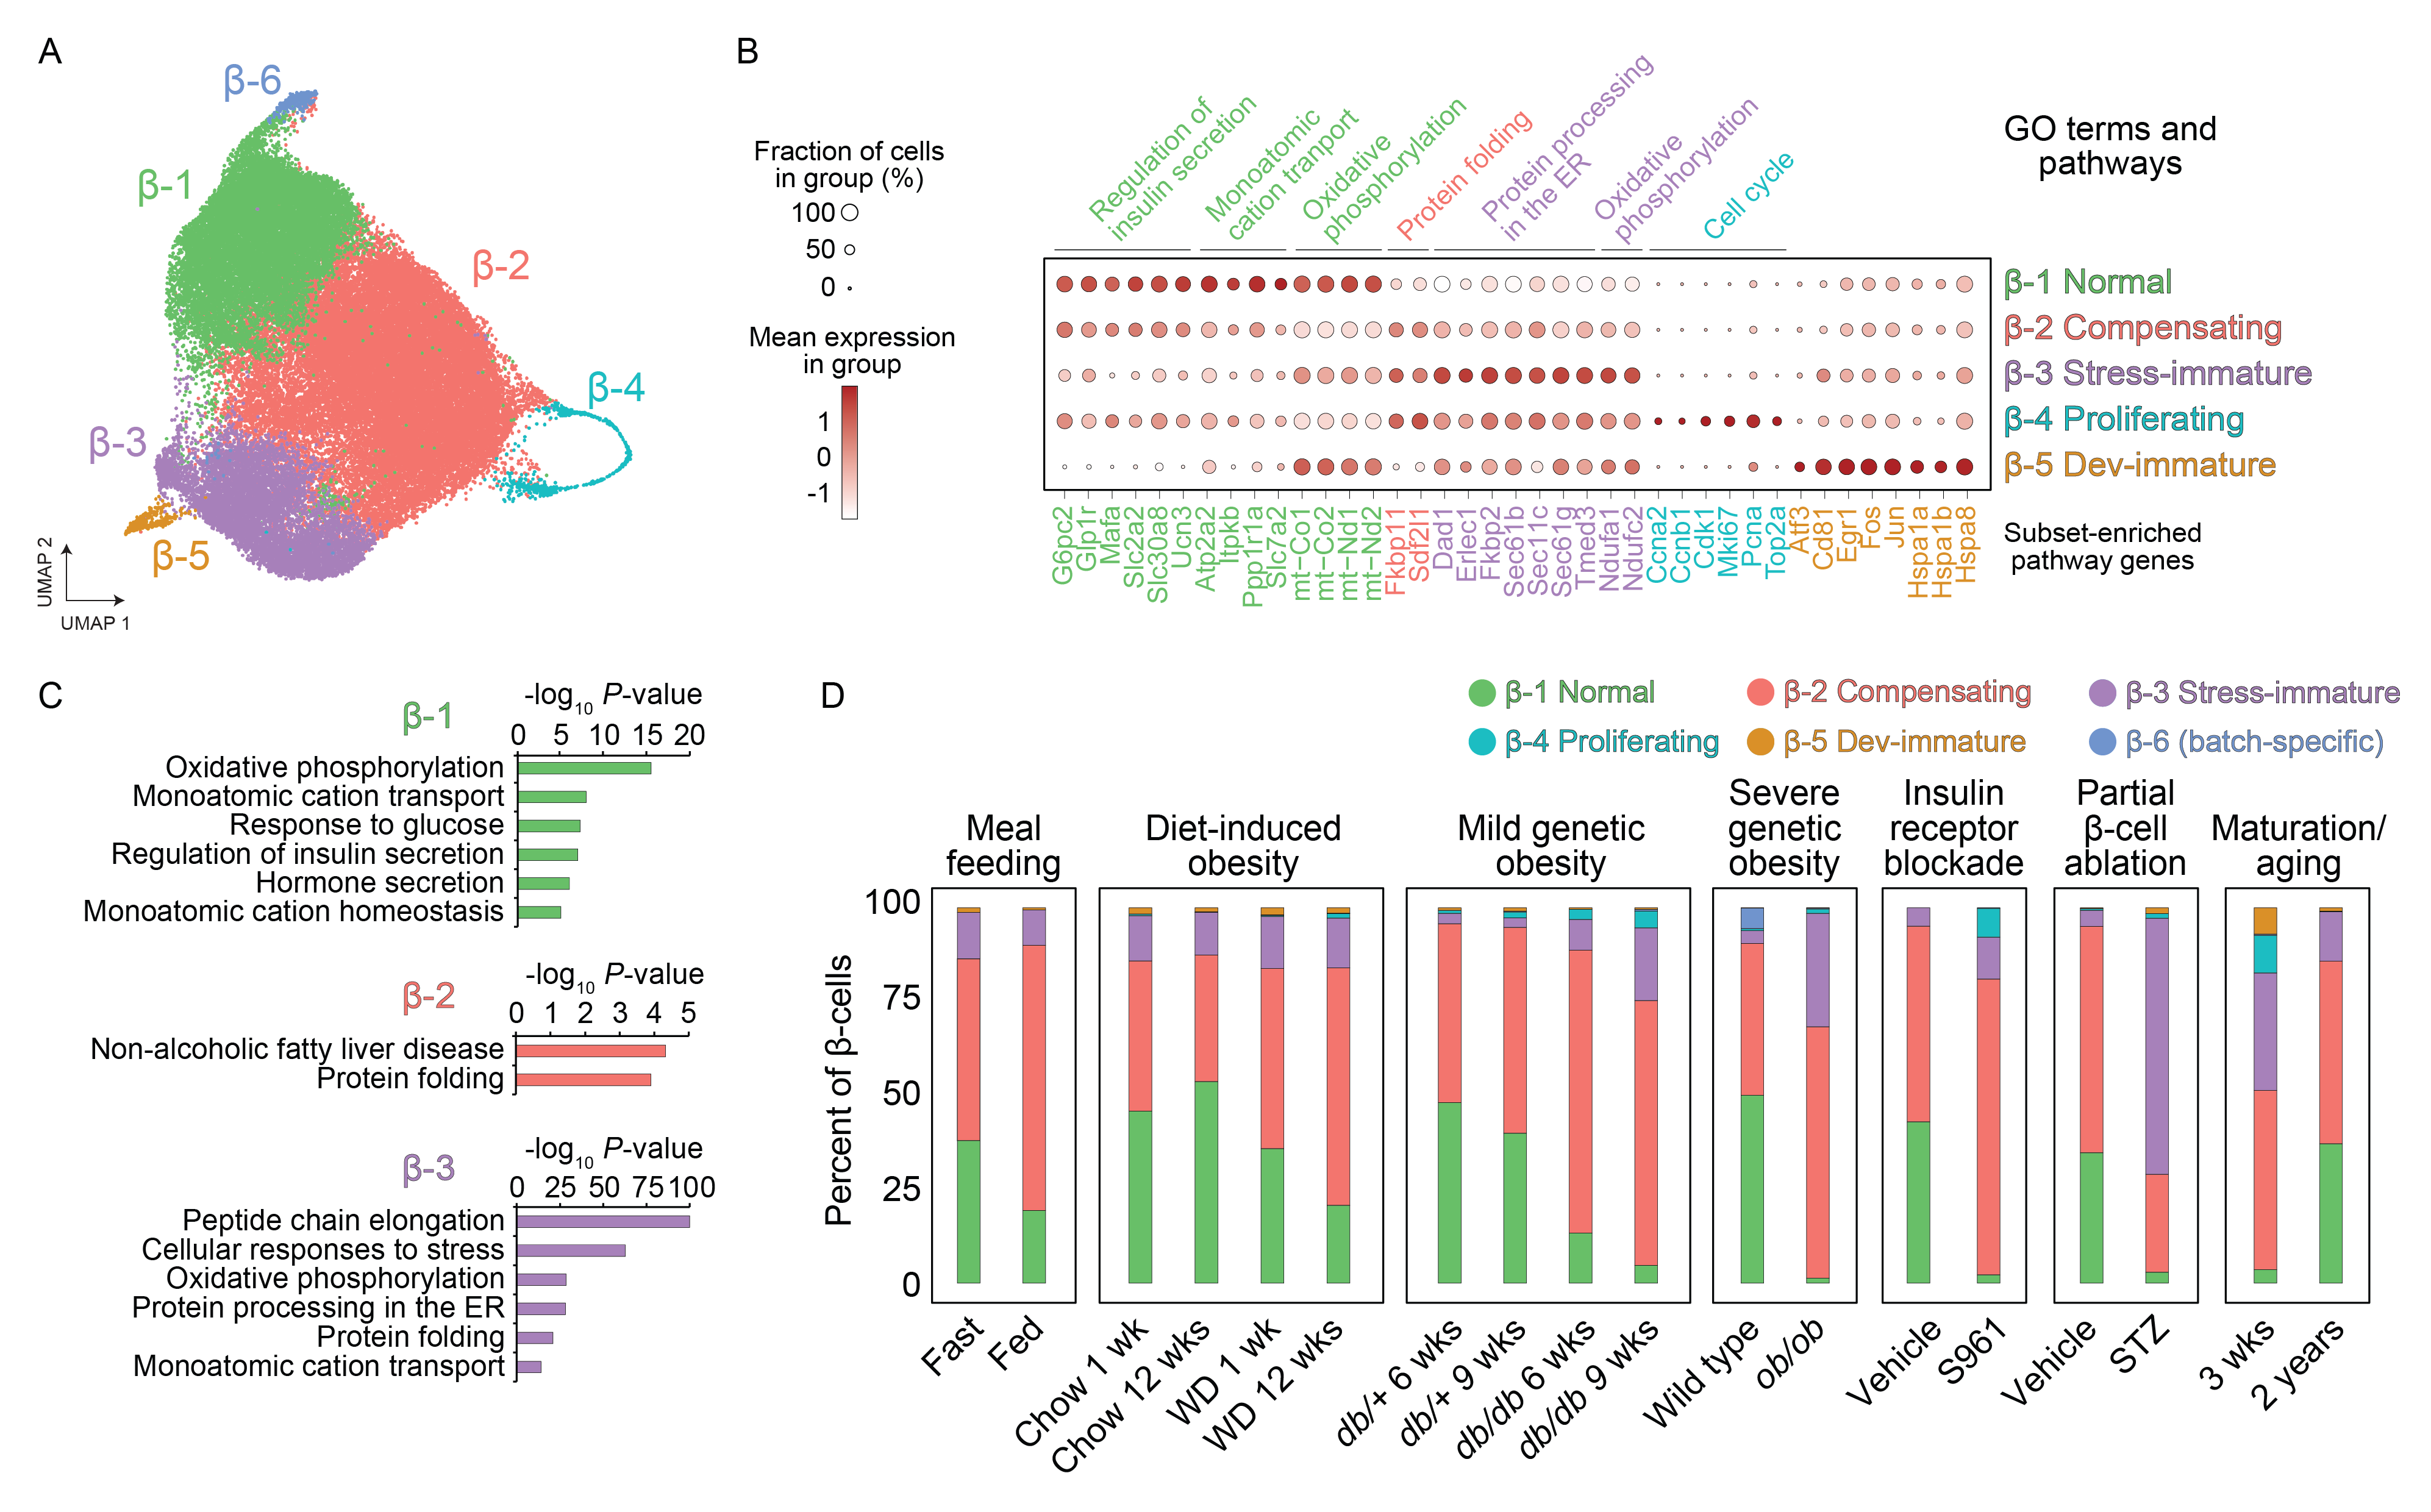
\includegraphics[width=\linewidth]{Chapter5/Fig/F3-1-v2-03.png}
% \caption[Characterization of $\beta$-cell subsets using enriched markers and \glslink{go}{GO} analysis]{\textbf{Characterization of $\beta$-cell subsets using enriched markers and \glslink{go}{GO} analysis.} \textbf{(A)} \gls{umap} embedding of the re-integrated $\beta$-cell subset, pooled from all experimental samples across the seven studies. The $\beta$-cells are grouped and colored according to the subsets identified via unsupervised clustering. \textbf{(B)} Dot plot depicting marker genes characteristic of each $\beta$-cell subset in panel (A). The marker genes are grouped according to the \gls{go} terms and pathways that they are associated with. The color of the dots represent the scaled average expression of the marker genes and the size of the dots correspond to the percentage of cells within the subset expressing the given marker gene. \textbf{(C)} Bar plots depicting enriched \gls{go} terms for $\beta$-1, $\beta$-2 and $\beta$-3 subsets. The significance ($-\log_{10}$ p-value) of the enrichment are shown. \textbf{(D)} The proportion of each $\beta$-cell subset in \textbf{(A)} computed as a percentage of total $\beta$-cell numbers in every experimental group.}
% \label{fig:chp3_betasubsets}
% \end{figure}

%Classification of $\beta$-cell subsets based on%gene ontology analysis of subset-enriched mRNAs
\par The original reports independently analyzing models at the single-cell level identified distinct subsets with transcriptomic differences relating to maturity and functional status of these $\beta$-cells. However, it is unclear how these subsets relate to each other across several models of $\beta$-cell decompensation and failure. Therefore, in order to define $\beta$-cell subsets in a more unified manner and to understand how changes in $\beta$-cell workload and glycemic dysregulation affect subset abundances, we classified $\beta$-cells into six putative subsets ($\beta$-1 through $\beta$-6) using unsupervised clustering \textbf{(\autoref{fig:chp3_betasubsets} A;} see \hyperref[subsubsec:met_chp3_betareint]{\textbf{Methods}}\textbf{)}. We then predicted cellular processes active in each cluster using \gls{go} and pathway analyses of marker genes associated with each cluster. Markers expressed highest in $\beta$-1 cells were enriched for \gls{go} terms and pathways such as \gls{oxphos} and regulation of insulin secretion, including previously described markers of $\beta$-cell maturity such as \textit{Mafa, Slc2a2}  and \textit{Ucn3}, and were therefore termed $\beta$-1 normal cells \textbf{(\autoref{fig:chp3_betasubsets} A-C)}. As expected, the $\beta$-1 cluster was enriched in the unchallenged controls of six studies (meal feeding, diet-induced obesity, mild and severe genetic obesity, insulin receptor blockade and partial $\beta$-cell ablation) as well as in the 2-year-old mice from the maturation/aging model \textbf{(\autoref{fig:chp3_betasubsets} D)}. The resemblance of $\beta$-cells from aged mice to the healthy and normal $\beta$-cells from younger mice has previously been demonstrated, with aging improving pancreatic $\beta$-cell function in mice \textbf{\cite{xin_single-cell_2016}}.\\ %This was also observed for the aging cohorts included in this atlas for which \gls{gsis} studies were conducted in \textbf{\autoref{chp:diet_aging}}. The aging cohorts demonstrated normal glucose tolerance and insulin sensitivity with their islet depicting heightened insulin release under basal and glucose-stimulated conditions in the \textit{in-vitro} culture.\\


\begin{figure}[t]
\centering
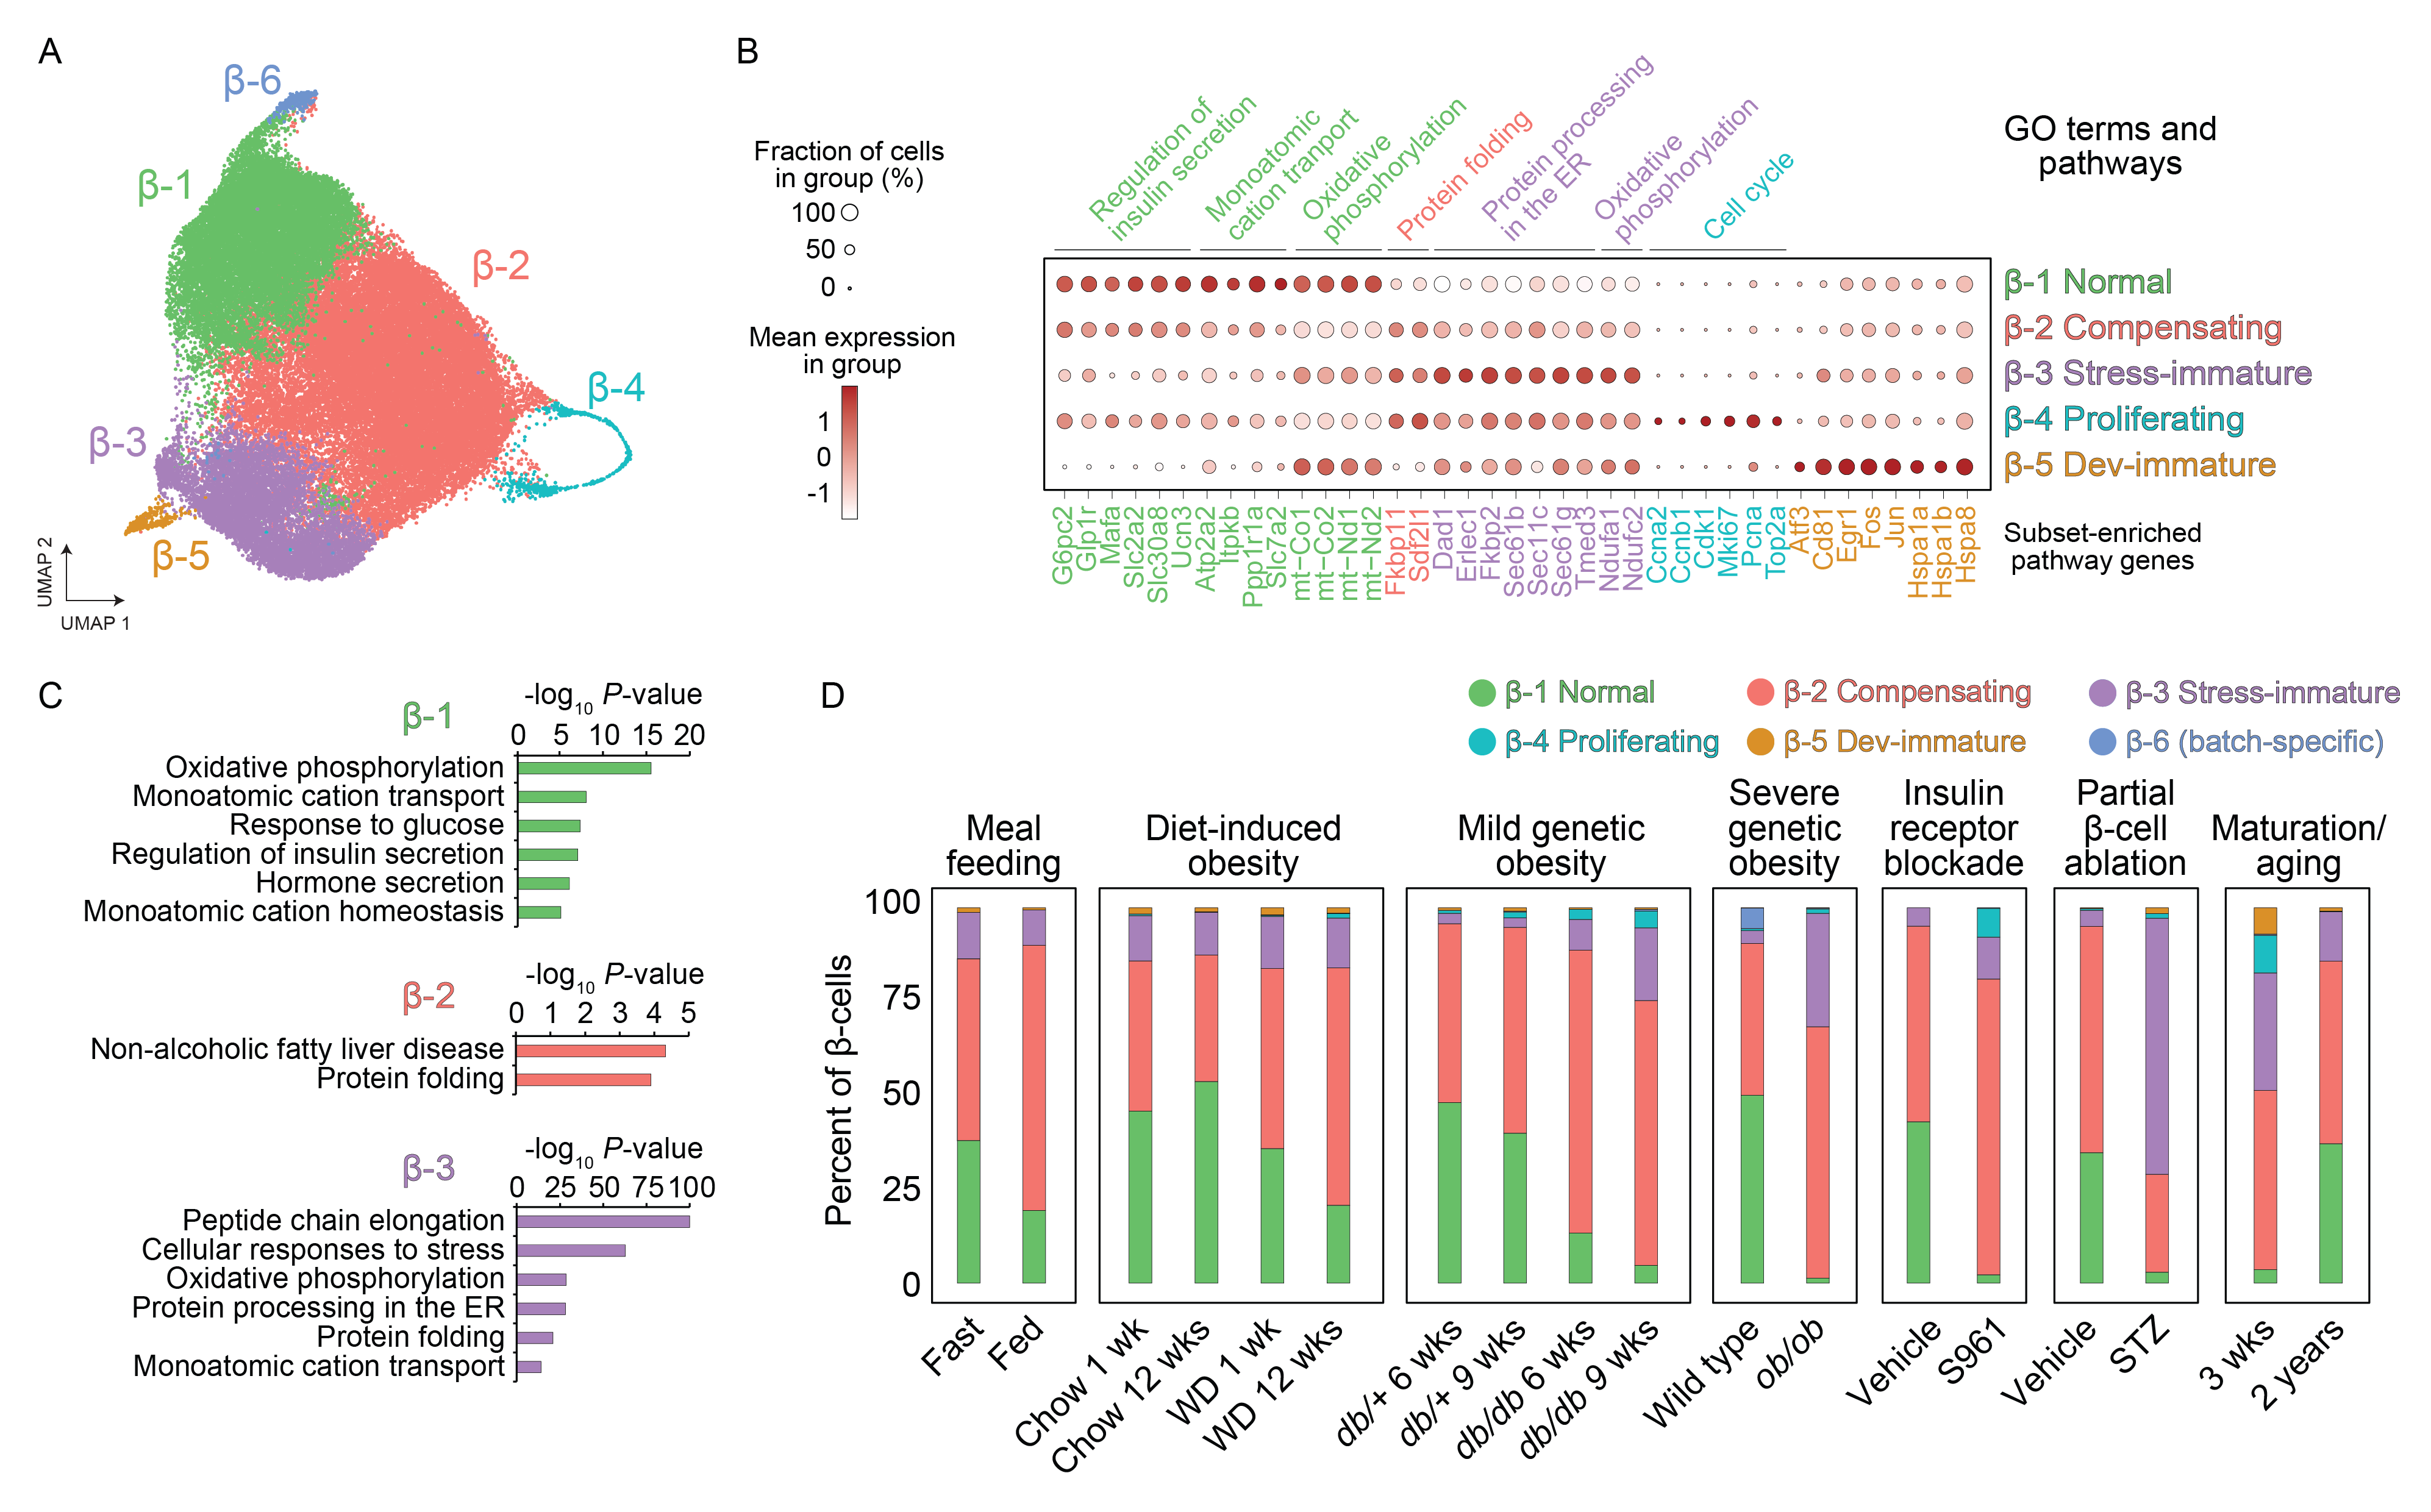
\includegraphics[width=\linewidth]{Chapter5/Fig/F3-1-v2-03.png}
\caption[Characterization of $\beta$-cell subsets using enriched markers and \glsentryshort{go} analysis]{\textbf{Characterization of $\beta$-cell subsets using enriched markers and \gls{go} analysis.} \textbf{(A)} \gls{umap} embedding of the re-integrated $\beta$-cell subset, pooled from all experimental samples across the seven studies. The $\beta$-cells are grouped and colored according to the subsets identified via unsupervised clustering. \textbf{(B)} Dot plot depicting marker genes characteristic of each $\beta$-cell subset in \textbf{(A)}. The marker genes are grouped according to the \gls{go} terms and pathways that they are associated with. The color of the dots represent the scaled average expression of the marker genes and the size of the dots correspond to the percentage of cells within the subset expressing the given marker gene. \textbf{(C)} Bar plots depicting enriched \gls{go} terms for $\beta$-1, $\beta$-2 and $\beta$-3 subsets. The significance ($-\log_{10}$ p-value) of the enrichment are shown. \textbf{(D)} The proportion of each $\beta$-cell subset in \textbf{(A)} computed as a percentage of total $\beta$-cell numbers in every experimental group. The cells from different biological replicate cohorts were pooled together. $\textsuperscript{**} p < 0.01, \textsuperscript{***} p < 0.001$. p-values were calculated from a mixed-effects binomial model.}
\label{fig:chp3_betasubsets}
\end{figure}

\par The $\beta$-5 subset expressed well-known markers of $\beta$-cell immaturity (\textit{e.g.} \textit{Cd81} \textbf{\cite{salinno_cd81_2021}}, \textit{Fos, Jun}) \textbf{(\autoref{fig:chp3_betasubsets} B)}. The $\beta$-5 subset was enriched in the young 3-week-old mice \textbf{(\autoref{fig:chp3_betasubsets} D)}, suggesting that this minor subset is composed of developmentally immature $\beta$-cells that are yet to establish a mature identity. We therefore termed this subset as $\beta$-5 developmental-immature ($\beta$-5 dev-immature).\\


\par The $\beta$-3 subset was characterized by expression of genes enriched in the \gls{go} term `cellular responses to stress' \textbf{(\autoref{fig:chp3_betasubsets} B,C)}. This subset was not enriched upon meal feeding compared to the fasting control or by an acute or chronic \gls{wd}, wherein the proportion of $\beta$-3 cells were similar to the corresponding chow diet fed controls \textbf{(\autoref{fig:chp3_betasubsets} D)}. In models of hyperglycemia, the proportion of the $\beta$-3 subset was strongly expanded in the challenged groups compared to their corresponding controls. This enrichment was strongest in the \gls{stz}-treated mice, which had the highest proportion of this cluster among all the other cohorts \textbf{(\ref{fig:chp3_betasubsets} D)}. This subset showed upregulation of genes involved in \gls{er} stress and \gls{oxphos} and is reminiscent of the immature $\beta$-cell subset originally reported to be enriched by \gls{stz} treatment \textbf{\cite{sachs_targeted_2020}}. Notably, the 3-week-old mice from the maturation/aging study also depicted an enrichment of the $\beta$-3 subset compared to the aged 2-year-old mice. Additionally, both the $\beta$-3 and $\beta$-5 cells showed strong subset-specific \gls{mrna} expression of \textit{Cd81}, which has been established as a known of $\beta$-cell immaturity and dedifferentiation \textbf{\cite{salinno_cd81_2021}}. Thus, the early developmental stage of 3-week-old mice seemed to align with the enrichment of the $\beta$-3 subset with signatures of stress-response and immaturity, in addition to the developmental immaturity associated with the $\beta$-5 subset. 
Based on these observations, we termed the $\beta$-3 subset as $\beta$-3 stress-immature, as the dedifferentiation of $\beta$-cells in this subset can likely be attributed to the metabolic stress response under conditions of severe hyperglycemia (and insulin resistance).\\

\par The $\beta$-2 subset constituted the largest proportion of $\beta$-cells and the analysis of the abundance of $\beta$-2 subset in all samples across the studies showed an almost universal enrichment with increasing $\beta$-cell workload \textbf{(\autoref{fig:chp3_betasubsets} D)}. This included the meal feeding model, which involved a 4-hour window of feeding or additional fasting. This likely suggests that the composition shift of $\beta$-2 observed in fed animals compared to fasted controls is quite rapid and involves changes in cellular state, as this shift outpaces estimates of $\beta$-cell turnover that would be necessary to impact abundances of cellular subsets. Similar enrichment of these $\beta$-2 compensating cells were observed in the 1-week and 12-week \gls{wd} fed obese adult animals as well as the 6-week-old and 9-week-old \textit{db/db} mice, which are not yet hyperglycemic. The majority of the islets of the hyperglycemic \textit{ob/ob} mice and the S961-treated mice were composed of the $\beta$-2 compensating subset \textbf{(\autoref{fig:chp3_betasubsets} D)}, which again indicated the severity of the workload experienced by the $\beta$-cells in these models. Genes expressed most highly in the $\beta$-2 subset were enriched for the \gls{go} term `protein folding' mainly comprising genes encoding \gls{er} resident proteins including chaperones and prolyl-isomerases \textbf{(\ref{fig:chp3_betasubsets} B,C)}. The up-regulation of \gls{er} machinery could signify an adaptive response to maintain \gls{er} homeostasis during increased requirements for insulin synthesis and processing during elevated $\beta$-cell workload. Genes over-expressed in the $\beta$-2 subset were expressed at intermediate levels in comparison to $\beta$-1 or $\beta$-3 cells \textbf{(\autoref{fig:chp3_betasubsets} B)}, and therefore $\beta$-2 associated genes were not as cluster-specific as genes characterizing $\beta$-1 or $\beta$-3 subsets. Overall, the observed composition shifts suggested that increases in $\beta$-cell workload gives rise to a state switch from $\beta$-1 normal state to $\beta$-2 compensating state.\\

\par Apart from the three major $\beta$-cell subsets and the minor $\beta$-5 dev-immature subset, the unsupervised clustering also identified two other subsets: $\beta$-4 subset expressing genes enriched for the \gls{go} terms `cell cycle’ and `DNA metabolic process’ including established markers of $\beta$-cell proliferation (\textit{Mki67, Top2a}). Therefore, we termed this subset as $\beta$-4 proliferating cells \textbf{(\autoref{fig:chp3_betasubsets} A,B; \autoref{fig:app_chp3_betasubsets} A)}. These cells were enriched in the young 3-week-old mice as well as in the S961-treated animals \textbf{(\autoref{fig:chp3_betasubsets} D)}. The S961-mediated increase in $\beta$-cell proliferation recapitulates prior findings \textbf{\cite{shirakawa_signaling_2023,wortham_metabolic_2024}}. Notably, we did not detect any proliferating $\beta$-cells in the meal feeding study or in the control mice of the insulin receptor blockade study. This absence is likely attributed to the stringent \gls{qc} thresholds applied during the analysis, along with the overall low cell counts in these models \textbf{(\autoref{fig:app_chp3_study} B; \autoref{tab:app_chp3_study})}. Nevertheless, we observed increases in the proportion of proliferating $\beta$-cells in response to increased workload across all other models analyzed \textbf{(\autoref{fig:chp3_betasubsets} D)}. Finally, $\beta$-6 comprised a minor subset, specific to the wild-type control for \textit{ob/ob} mice in the severe genetic obesity study \textbf{(\autoref{fig:chp3_betasubsets} D; \autoref{fig:app_chp3_betasubsets} B,C)}. However, it is unclear what this small subset might represent. Of note, the gene module analysis identified module \textit{M8}, which was highly and specifically expressed in this wild-type sample \textbf{(\autoref{fig:chp3_pseudobulk} B)}, and the transcriptional profile of the module \textit{M8} was similar to GP25 in the \gls{mia}.\\

\begin{wrapfigure}{r}{0.6\textwidth}
\vspace{-15pt}
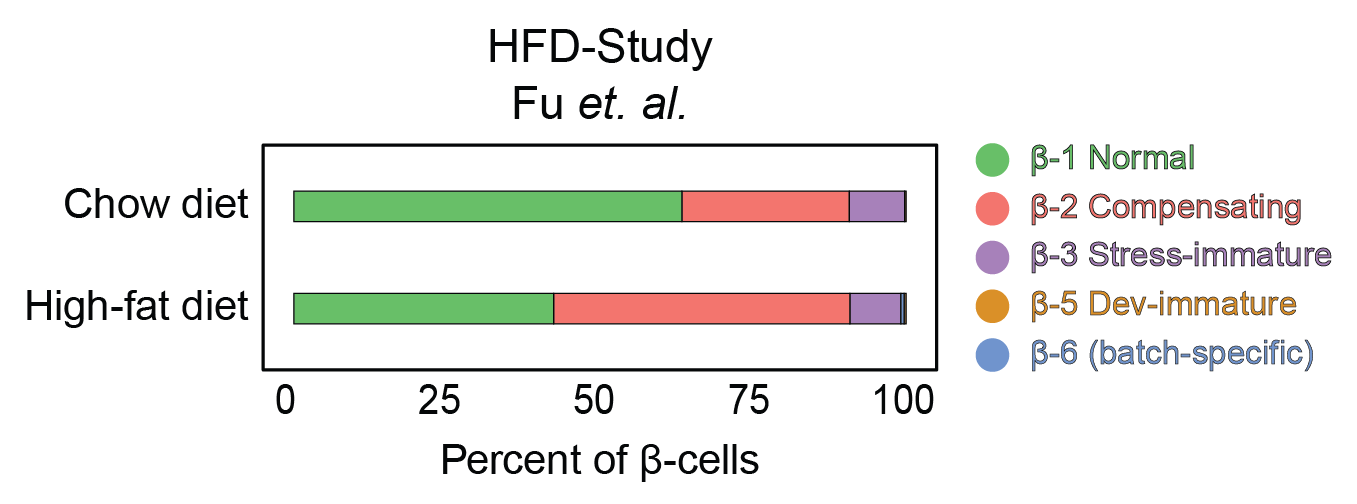
\includegraphics[width=9cm]{Chapter5/Fig/F3-1-v2-04.png}
\caption[Mapping integrated $\beta$-cell subset onto an external \glsentryshort{hfd} study]{\textbf{Mapping integrated $\beta$-cell subset onto an external \gls{hfd} study}. Bar plot depicting the composition shifts of $\beta$-cell subsets between the Chow diet and \gls{hfd} in an external \gls{scr} study \textbf{\cite{fu_single-cell_2023}}. The $\beta$-cells in this external study were re-annotated as $\beta$-cell subsets from the integrated reference following the label transfer workflow.}
\vspace{-8pt}
\label{fig:chp3_hfdmapping}
\end{wrapfigure}


\par We also performed a comparative analysis by mapping an external, independent \gls{scr} study onto our integrated  $\beta$-cell subset. This dataset was obtained from islets from mice subjected to \gls{hfd} induced glucose intolerance \textbf{(\autoref{tab:app_chp3_study};} see \hyperref[subsubsec:met_chp3_data]{\textbf{Methods}}\textbf{)} \textbf{\cite{fu_single-cell_2023}}. We mapped the $\beta$-cells from this external study onto our annotated $\beta$-cell subset, which enabled us to: \textbf{(i)} re-annotate the $\beta$-cells from the \gls{hfd}-study with the subset annotations from our integrated atlas and \textbf{(ii)} compare the compositional changes of the $\beta$-cell subsets in a \gls{hfd}-induced obesity model of metabolic stress \textbf{(}see \hyperref[subsubsec:met_chp3_validation]{\textbf{Methods}}\textbf{)}. Similar to \gls{wd} feeding, \gls{hfd} feeding resulted in the shift of subset composition, with the proportion of the $\beta$-1 normal subset reduced after 8-week \gls{hfd} feeding \textbf{(\autoref{fig:chp3_hfdmapping})}. This was accompanied by an increase in the proportion of the $\beta$-2 compensating subset in the \gls{hfd}-fed mice \textbf{(\autoref{fig:chp3_hfdmapping})}. The proportion of $\beta$-3 subset remain unchanged between chow diet and \gls{hfd} \textbf{(\autoref{fig:chp3_hfdmapping})}. This invariance of the stress-immature subset was also observed in our integrated atlas, in the case of meal feeding and \gls{wd}-induced obesity \textbf{(\autoref{fig:chp3_betasubsets} D)}, reflective of successful adaptation of $\beta$-cells to increased workloads in these models.\\


%\hl{<ERAD and UPR scores>}\\
In summary, unsupervised clustering of $\beta$-cells revealed six $\beta$-cell subsets that were annotated based on cellular processes which were characteristic of each subset. We identified a $\beta$-1 normal subset with known markers of maturity and function and a $\beta$-3 stress-immature subset which depicted markers of stress response as well as immaturity. We additionally identified a small developmentally immature $\beta$-5 subset which can be distinguished from the $\beta$-1 normal subset using previously described markers. Taken together, this likely suggests that $\beta$-cell immaturity can be associated with developmental or stress-response processes. We also identified a proliferative $\beta$-4 subset expressing genes involved in DNA replication and cell division. The majority of $\beta$-cells were compensatory or adaptive in nature, which showed an universal enrichment in response to increasing $\beta$-cell workload. Interestingly, this $\beta$-2 compensating subset lacked any specific markers unlike the $\beta$-1 or $\beta$-3 subsets, possibly suggesting that this subset could correspond to a continuum of $\beta$-cell phenotype related to workload. 

%\clearpage

\section[$\beta$-cell dysfunction corresponds to increased workload concomitant with loss of maturation]{$\beta$-cell dysfunction corresponds to increased workload\\concomitant with loss of maturation}
\label{sec:chp3_betaPCA}

In the above analyses, we identified three major $\beta$-cell subsets ($\beta$-1 normal, $\beta$-2 compensating and $\beta$-3 stress-immature) with subset-specific genes that were enriched for distinct cellular processes. Furthermore, these subsets exhibited compositional shifts in response to increasing $\beta$-cell workload. However, it is unknown whether these subsets represent discrete or continuous states, and the relationship between them is unclear. Additionally, as the over-expressed genes in the $\beta$-2 compensating subset were not cluster-specific compared to the $\beta$-1 or $\beta$-3 subsets, we hypothesized that this compensating state might form a continuum between the other two major subsets. Therefore, to further assess the subset annotations of islet $\beta$-cells and their compositional shifts in response to increased workload in hyperglycemic and insulin-resistant models, we utilized \gls{pca} \textbf{\cite{pearson_lines_1901}}.\\



\begin{wrapfigure}{l}{0.55\textwidth}
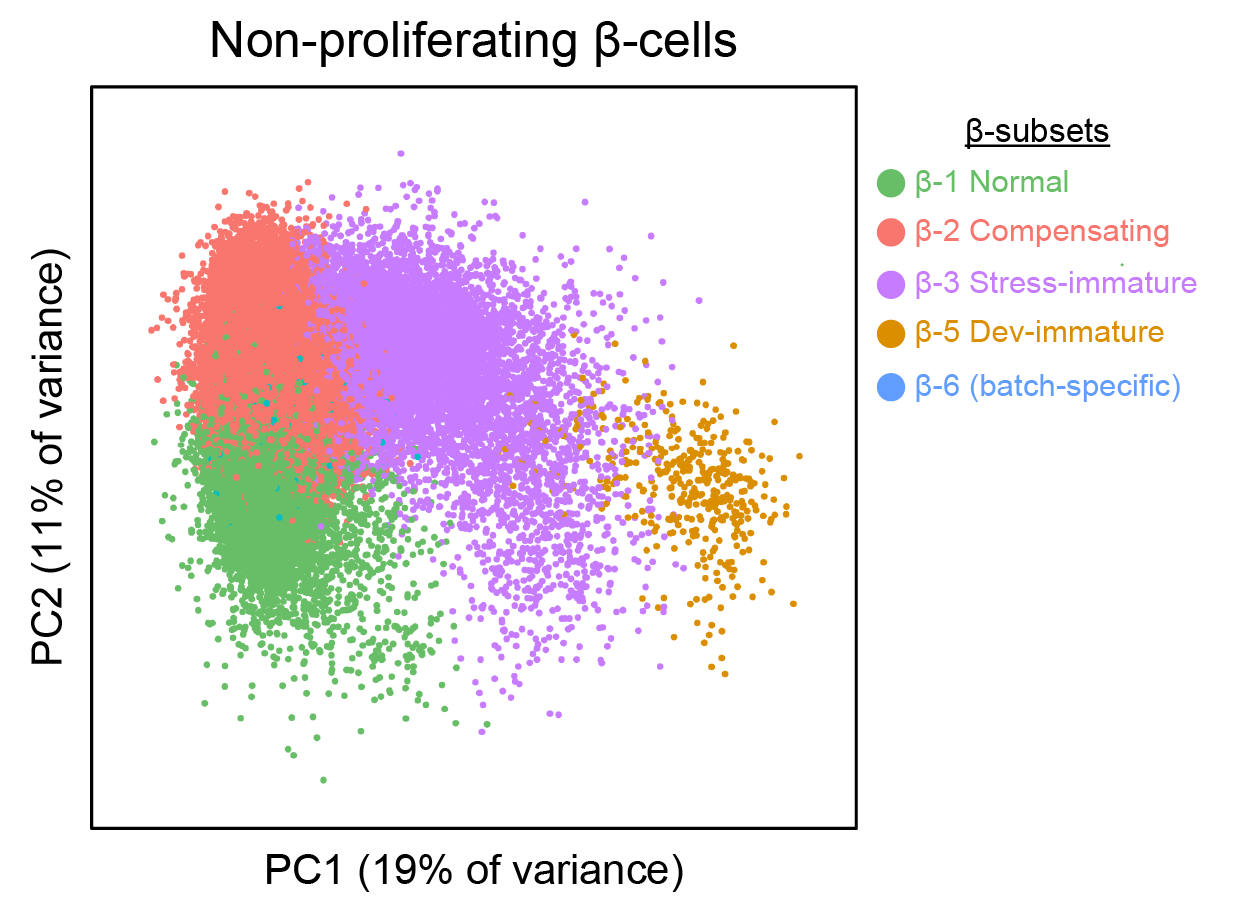
\includegraphics[width=8cm]{Chapter5/Fig/F3-6-01.png}
\caption[\glsentryshort{pca} of non-proliferating $\beta$-cell subsets]{\textbf{\gls{pca} of non-proliferating $\beta$-cell subset.} \gls{pc} embedding of the re-integrated, non-proliferating $\beta$-cell subset, pooled from all experimental samples across the seven studies. The $\beta$-cells are grouped and colored according to the five non-proliferating $\beta$-cell subsets.}
\label{fig:chp3_pca}
\end{wrapfigure}

\par In theory, each \acrfull{pc} represents an axis in a high-dimensional space that captures the largest amount of variation in the data. Thus, the first \gls{pc} maximizes this variance and the second \gls{pc} captures most of the remaining amount of variation and is orthogonal to the first \gls{pc}. In the context of \gls{scr}, it is widely assumed that biological processes affect multiple genes in a coordinated manner whereas random or biological noise would affect each gene independently. Therefore, it is common practice in \gls{scr} to make use of earlier and top \glspl{pc} in downstream analysis. This is a simple, highly-effective and widely used strategy in several fields \textbf{\cite{noauthor_dimensionality_nodate}}.\\

% \vspace{100pt}

%\st{Therefore, the earlier PCs are more likely represent the biological heterogeneity whereas the technical variability would be attributed with later PCs.}


\par We recomputed the \glspl{pc} for all the non-proliferating $\beta$-cells in the re-integrated subset \textbf{(}see \hyperref[subsubsec:met_chp3_pca]{\textbf{Methods}}\textbf{)}. The dynamic changes in gene expression during cell cycle phases exhibits high variation in the \glspl{pc}, which can obscure underlying biological differences. Thus, to avoid confounding effects from cell cycle-related gene expression, we excluded proliferating $\beta$-cell subset and focused on non-proliferating $\beta$-cells for downstream analysis. In our analysis, the first two \glspl{pc} (\gls{pc}1 and \gls{pc}2) were distinguished the three major $\beta$-cell subsets \textbf{(\autoref{fig:chp3_pca})}. Across the 3000 \glspl{hvf}, \gls{pc}1 accounted for 19\% of the variance \textbf{(\autoref{fig:chp3_pca})} and corresponded with $\beta$-cell maturation state \textbf{(\autoref{fig:chp3_pc1}; \autoref{fig:app_chp3_pc1})}. This was evident from a histogram plot depicting cell densities across the \gls{pc}1 weights along which the cells were ordered \textbf{(}see \hyperref[subsubsec:met_chp3_pca]{\textbf{Methods}}\textbf{)}. Traversing along this ranked axis, we observed that the $\beta$-3 stress-immature \textbf{(\autoref{fig:chp3_pc1} A)} and the $\beta$-5 dev-immature subsets \textbf{(\autoref{fig:app_chp3_pc1} A)} accounted for the higher density and were distinguished from the $\beta$-1 normal or $\beta$-2 compensating subsets.\\


\par Shifted distributions of cells along \gls{pc}1 across the experimental interventions suggested that the loss of $\beta$-cell maturity occurred in models with systemic hyperglycemia and failed adaptation \textit{i.e.}, in the \textit{ob/ob} mice and following S961- or \gls{stz}-treatment \textbf{(\autoref{fig:app_chp3_pc1} B,} bottom row\textbf{)}. This was in contrast to the modest interventions that resulted in successful $\beta$-cell adaptation, wherein there were minor differences of the $\beta$-cell maturity axis with feeding, \gls{wd}-induced obesity or in the \textit{db/db} mice \textbf{(\autoref{fig:app_chp3_pc1} B,} top row\textbf{)}. Overall, this observation supports the notion that $\beta$-cell decompensation associates with loss of maturity. In addition to the up-regulation of genes involved in \gls{oxphos} and protein processing in the \gls{er} in $\beta$-3 subset \textbf{(\autoref{fig:chp3_betasubsets} B)}, \gls{pc}1 also corresponded to the up-regulation of ribosomal protein genes \textbf{(\autoref{fig:chp3_pc1} B,C)}.\\ %\st{This could be explained by a higher demand for protein synthesis in $\beta$-3 subset in order to adapt to increased workload demands associated with hyperglycaemic environment and $\beta$-5 subset wherein cells could be producing a large number of ribosomes in order to support the synthesis of proteins required for maturation.}\\


\begin{figure}[t]
\centering
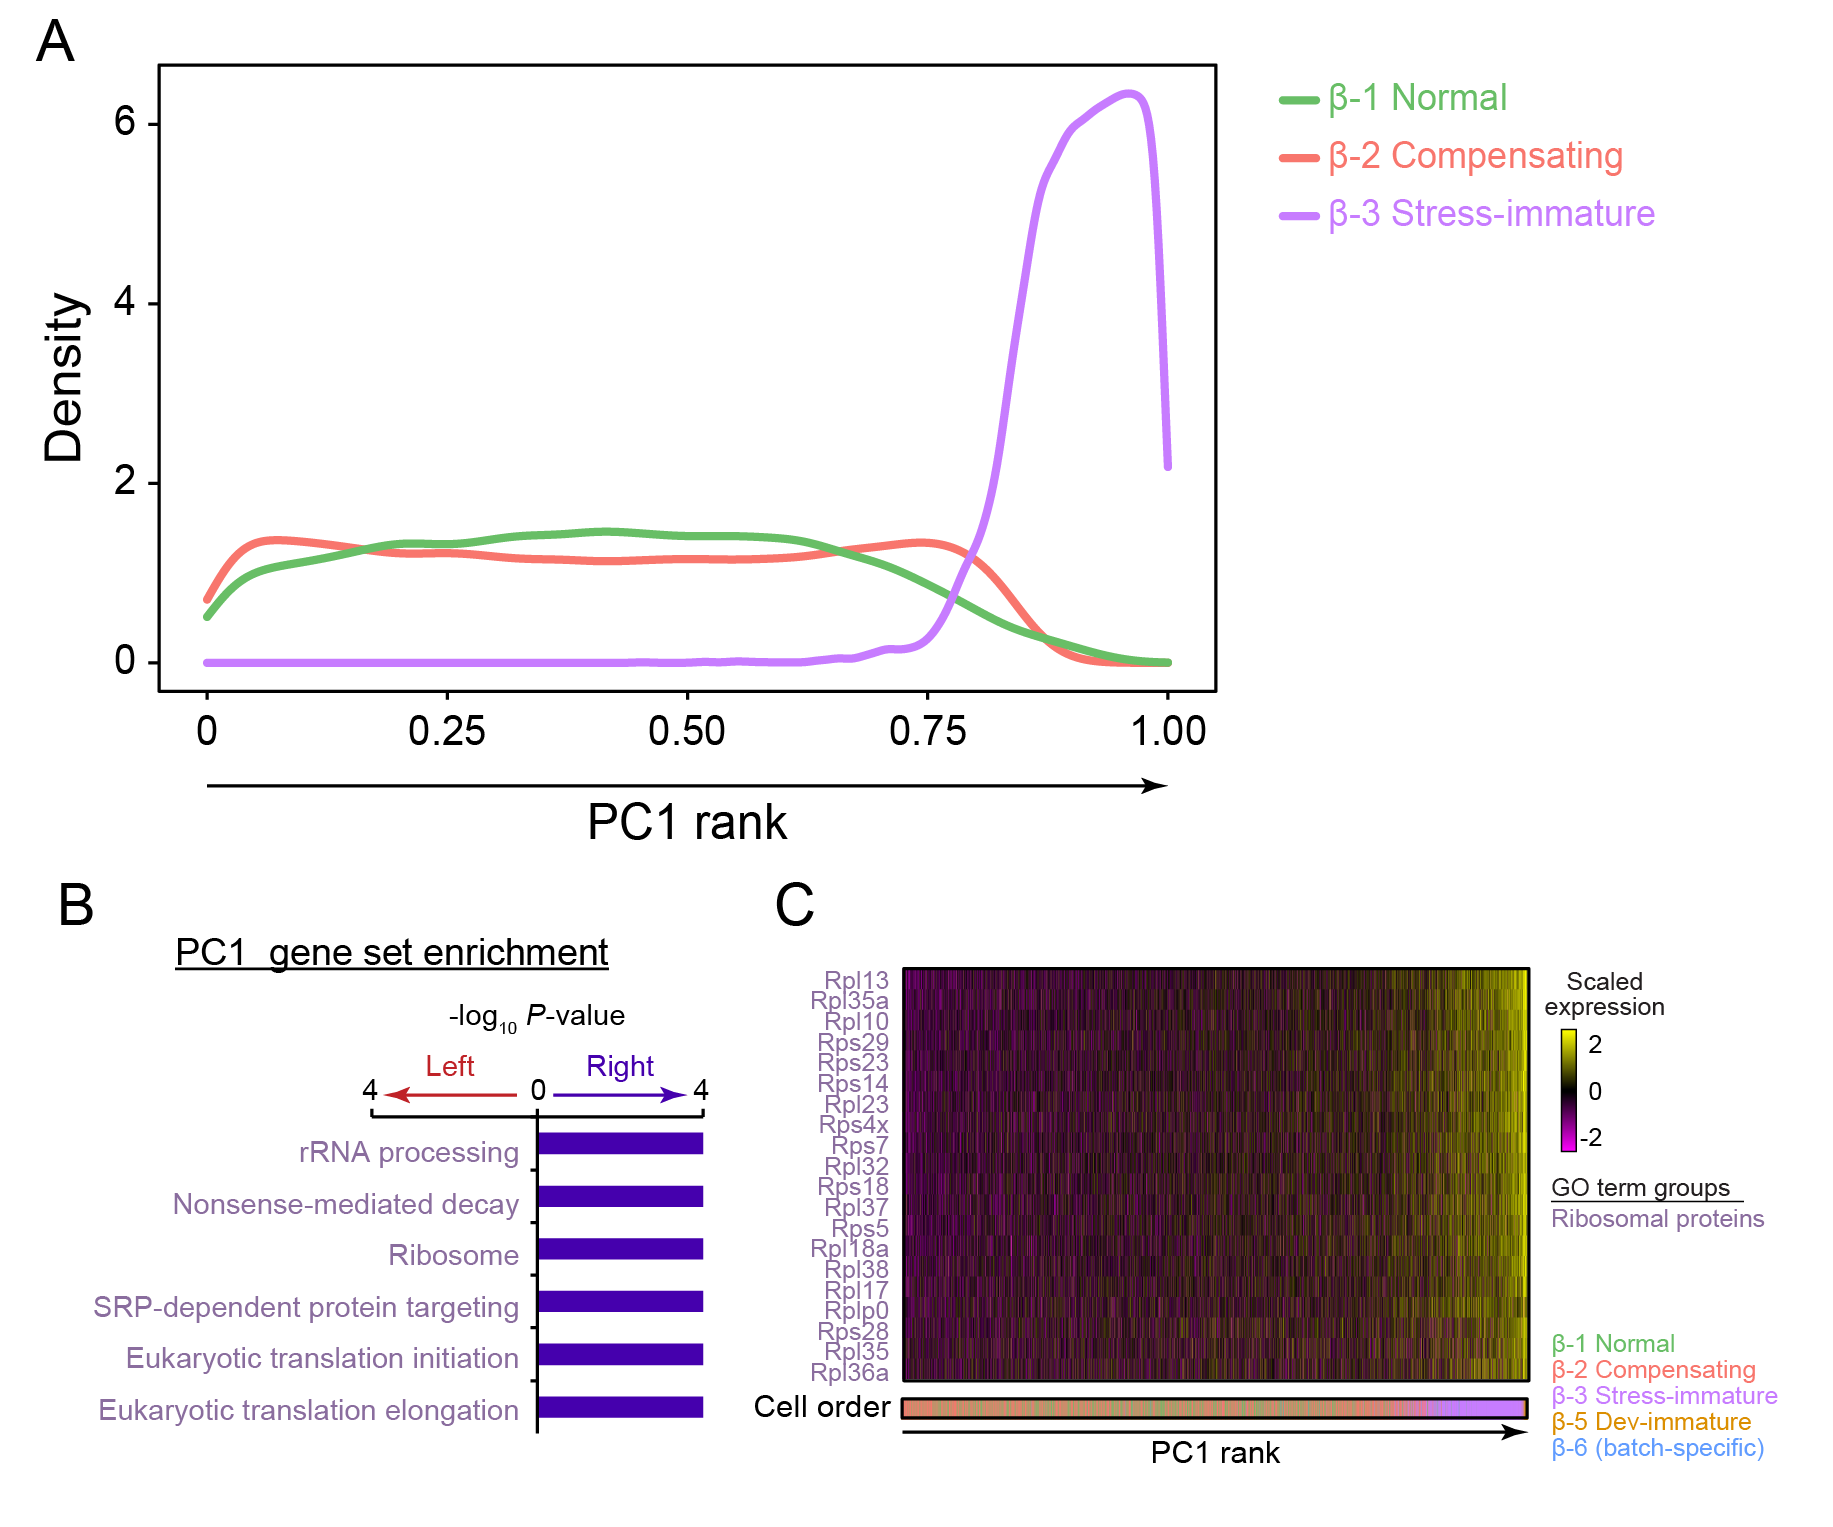
\includegraphics[width=\linewidth]{Chapter5/Fig/F3-6-02}
\caption[Deteriorating glucose homeostasis associates with \glsentryshort{pc}1]{\textbf{Deteriorating glucose homeostasis associates with \gls{pc}1.} \textbf{(A)} Density plot depicting the distribution of the three major $\beta$-cell subsets as curves along normalized \gls{pc}1 rank. \textbf{(B)} \gls{gsea} of top 500 genes that were associated with \gls{pc}1. The significance ($-\log_{10}$ p-value) of the enrichment are shown in bar plots. \textbf{(C)} Heatmap depicting the scaled expression of the indicated ribosomal genes (rows) across all non-proliferating $\beta$-cells ordered according to their ranks along \gls{pc}1. The color bar below the heatmap indicates the subset annotations.}
% \vspace{-15pt}
\label{fig:chp3_pc1}
\end{figure}



\begin{figure}[t]
\centering
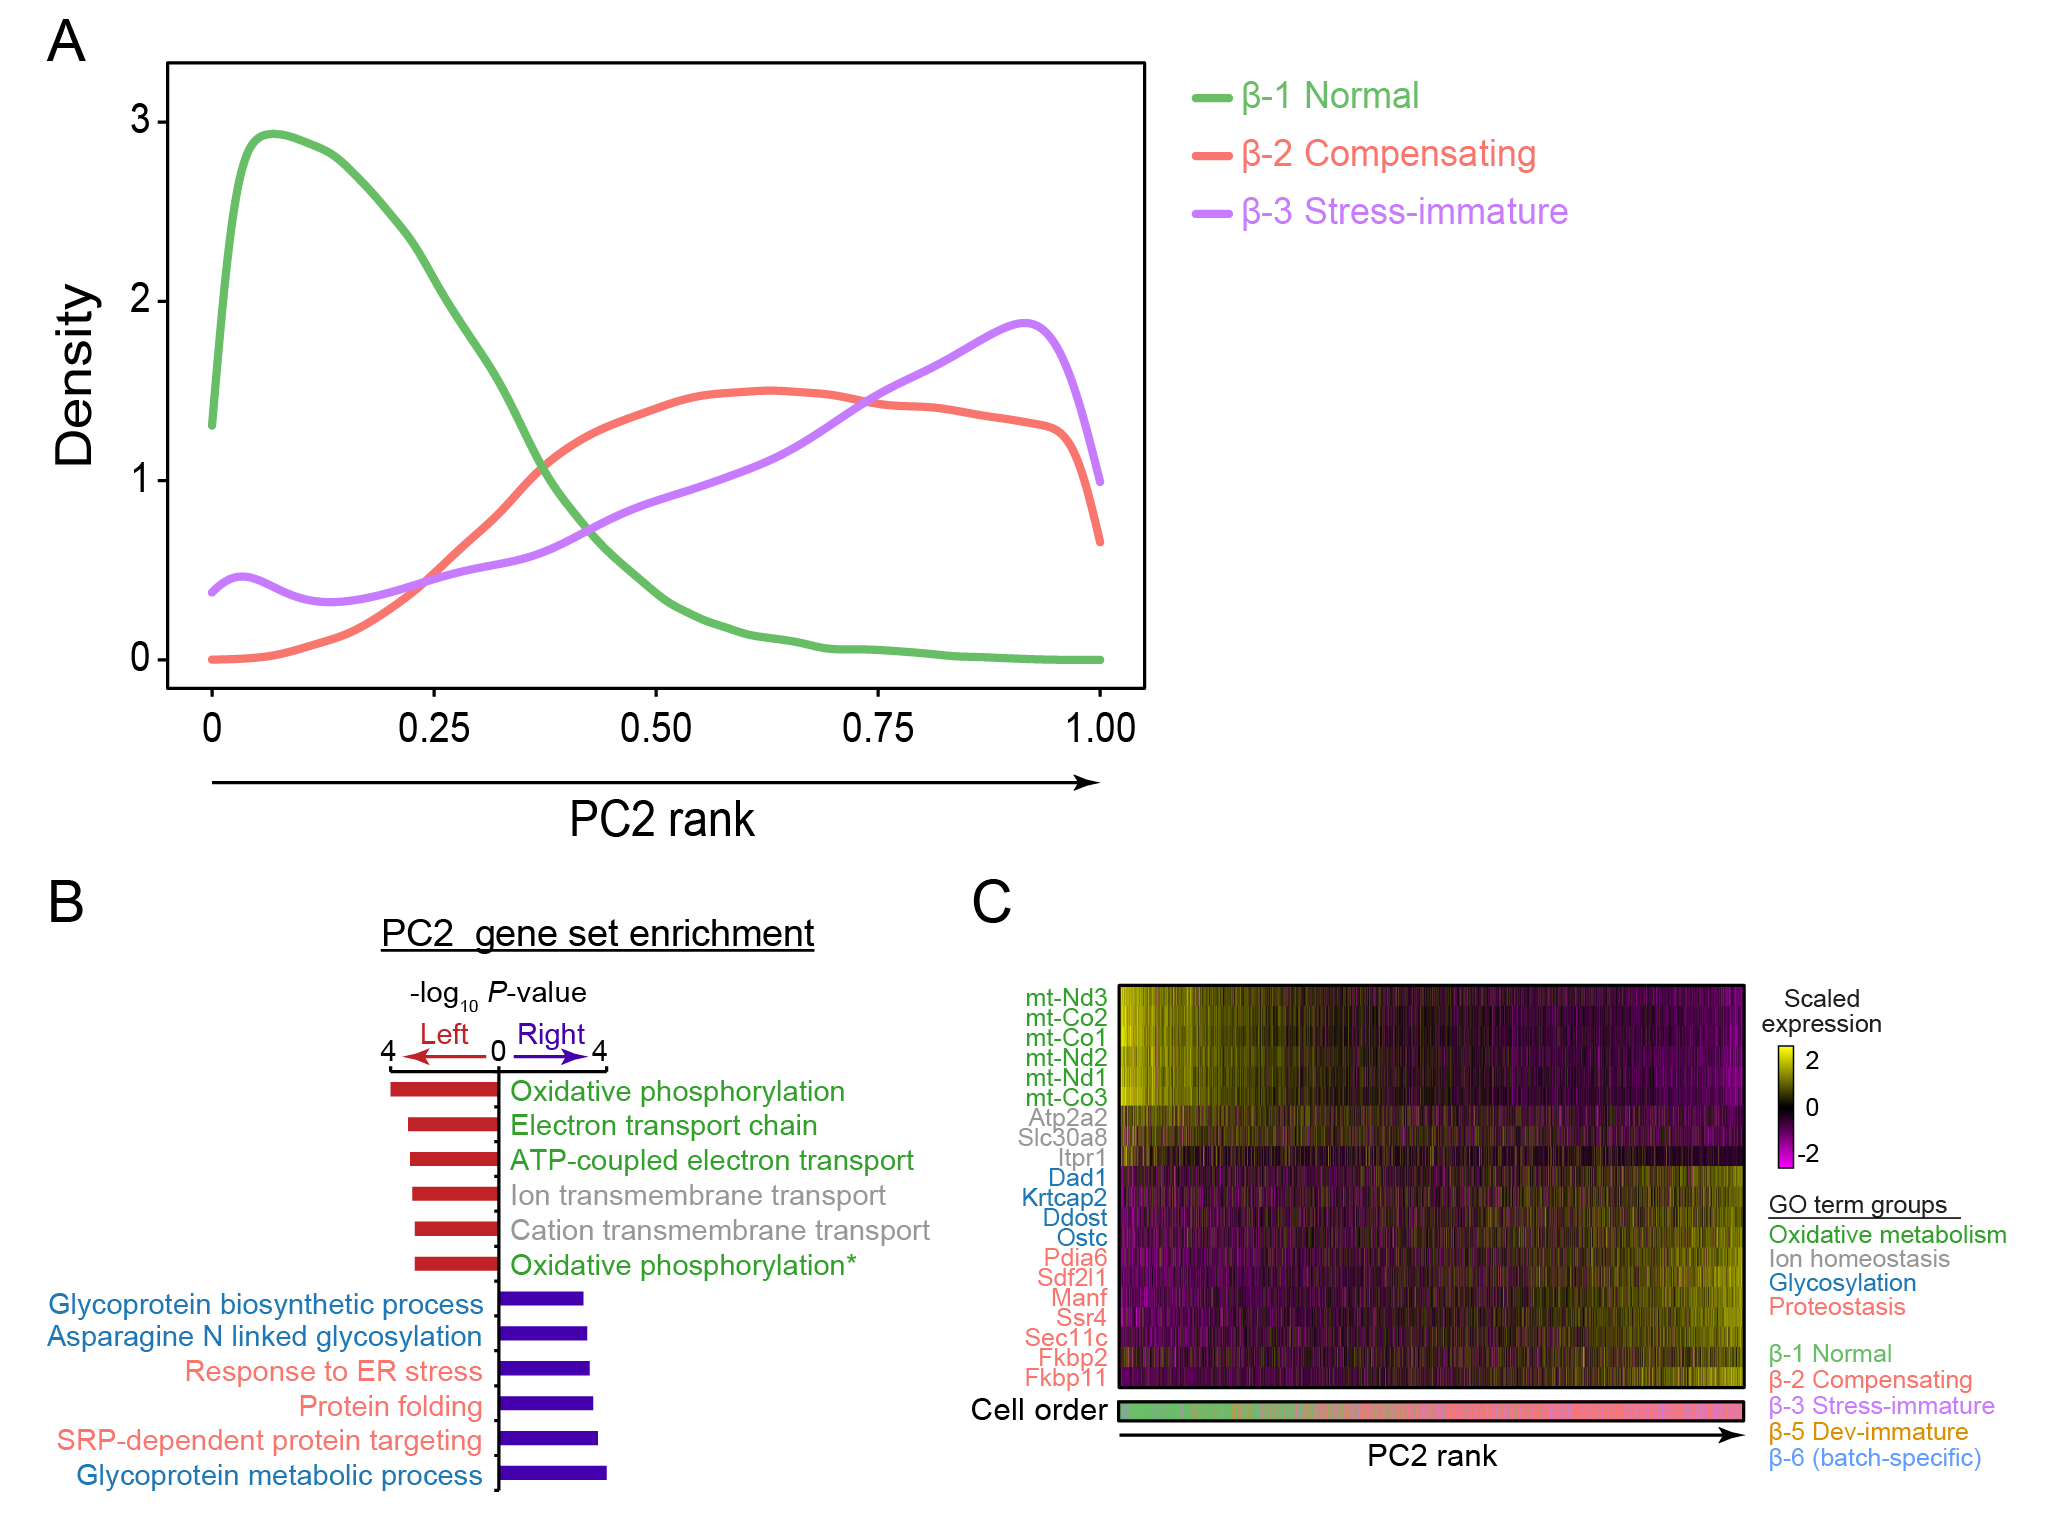
\includegraphics[width=\linewidth]{Chapter5/Fig/F3-6-03}
\caption[Increased $\beta$-cell workload associates with \glsentryshort{pc}2]{\textbf{Increased $\beta$-cell workload associates with \gls{pc}2.} \textbf{(A)} Density plot depicting the distribution of the three major $\beta$-cell subsets as curves along normalized \gls{pc}2 rank. \textbf{(B)} \gls{gsea} of top 500 genes that were associated with \gls{pc}2. The significance ($-\log_{10}$ p-value) of the enrichment are shown in bar plots. \textbf{(C)} Heatmap depicting the scaled expression of the indicated genes associated with oxidative metabolism, ion homeostasis, glycosylation and proteostasis (rows) across all non-proliferating $\beta$-cells ordered according to their ranks along \gls{pc}2. The color bar below the heatmap indicates the subset annotations.}
\label{fig:chp3_pc2}
\end{figure}

%\clearpage

\par On the other hand, \gls{pc}2 explained 12\% of the variance across $\beta$-cell subsets \textbf{(\autoref{fig:chp3_pca})} and corresponded with increased insulin demand per $\beta$-cell \textbf{(\autoref{fig:chp3_pc2}, \autoref{fig:app_chp3_pc2})}. The ranked density plot of $\beta$-cells ordered by their \gls{pc}2 weights distinguished $\beta$-1 normal from $\beta$-2 or $\beta$-3 subsets \textbf{(\autoref{fig:chp3_pc2} A;} see \hyperref[subsubsec:met_chp3_pca]{\textbf{Methods}}\textbf{)}. Interestingly, the distribution of the $\beta$-5 dev-immature subset along \gls{pc}2 overlapped with $\beta$-1 normal subset which suggested developmental immaturity is not associated with increased workload, in all the models included in this atlas \textbf{(\autoref{fig:app_chp3_pc2} A)}. Furthermore, the distributions across the \gls{pc}2 was shifted for all experimental interventions, including fasting and re-feeding \textbf{(\autoref{fig:app_chp3_pc2} B,C)}. Thus, \gls{pc}2 described the extent of workload with respect to any model that increased insulin demand on a per $\beta$-cell basis, which can be impacted through either altered insulin sensitivity or altered $\beta$-cell numbers. Compared to \gls{pc}1, diverse gene sets were associated with \gls{pc}2 progression, with the apparent repression of mitochondrial-encoded components of the electron transport chain and up-regulation of genes involved in proteostasis, glycosylation machinery and response to \gls{er} stress \textbf{(\autoref{fig:chp3_pc2} B,C)}.\\ 

\par Consequently, we scored for canonical \gls{erad} and \gls{upr} genes across all major non-proliferating $\beta$-subsets \textbf{(}see \hyperref[subsubsec:met_chp3_scoring]{\textbf{Methods}}\textbf{)}. The \gls{erad} and \gls{upr} processes play an indispensable role in mitigating \gls{er} stress, restoring cellular homeostasis and maintaining $\beta$-cell identity and function \textbf{\cite{oppenlander_vertical_2021}}. We observed that the expression score for both \gls{erad} and \gls{upr} processes was higher in the $\beta$-2 compensating and the $\beta$-3 stress-immature subsets compared to the $\beta$-1 normal cells \textbf{(\autoref{fig:chp3_eradupr})}. This reflects the transition from a homeostatic to pathological role for both of these cellular pathways in response to chronic workloads. Interestingly, the $\beta$-5 dev-immature subsets exhibited lower \gls{erad} and \gls{upr} scores compared to the other three $\beta$-cell subsets \textbf{(\autoref{fig:chp3_eradupr})}. This could reflect different cellular strategies for managing protein folding and stress that are distinct from the heightened responses observed in compensating or stressed $\beta$-cells. Furthermore, the up-regulation of \gls{erad} and \gls{upr} processes was coupled to each other in response to interventions in each dataset \textbf{(\autoref{fig:app_chp3_eradupr})}. Of note, the partial $\beta$-cell ablation model did not depict a strong up-regulation of the \gls{upr} score compared to the \gls{erad} score in the same model. The lack of adaptive \gls{upr} in the \gls{er} of $\beta$-cells in this model could serve as a critical role for dedifferentiation in these $\beta$-cells \textbf{\cite{sachs_targeted_2020,khin_brief_2021}}.\\

%We speculate these changes reflect activation of a program intended to preserve ER homeostasis when each cell is attempting to produce and secrete increasing amounts of insulin.\\ observed patterns of \gls{erad} and \gls{upr} scores across $\beta$-cell subsets aligned with the overall up-regulation in response to the

%clearpage

% \begin{wrapfigure}{l}{0.7\textwidth}
% 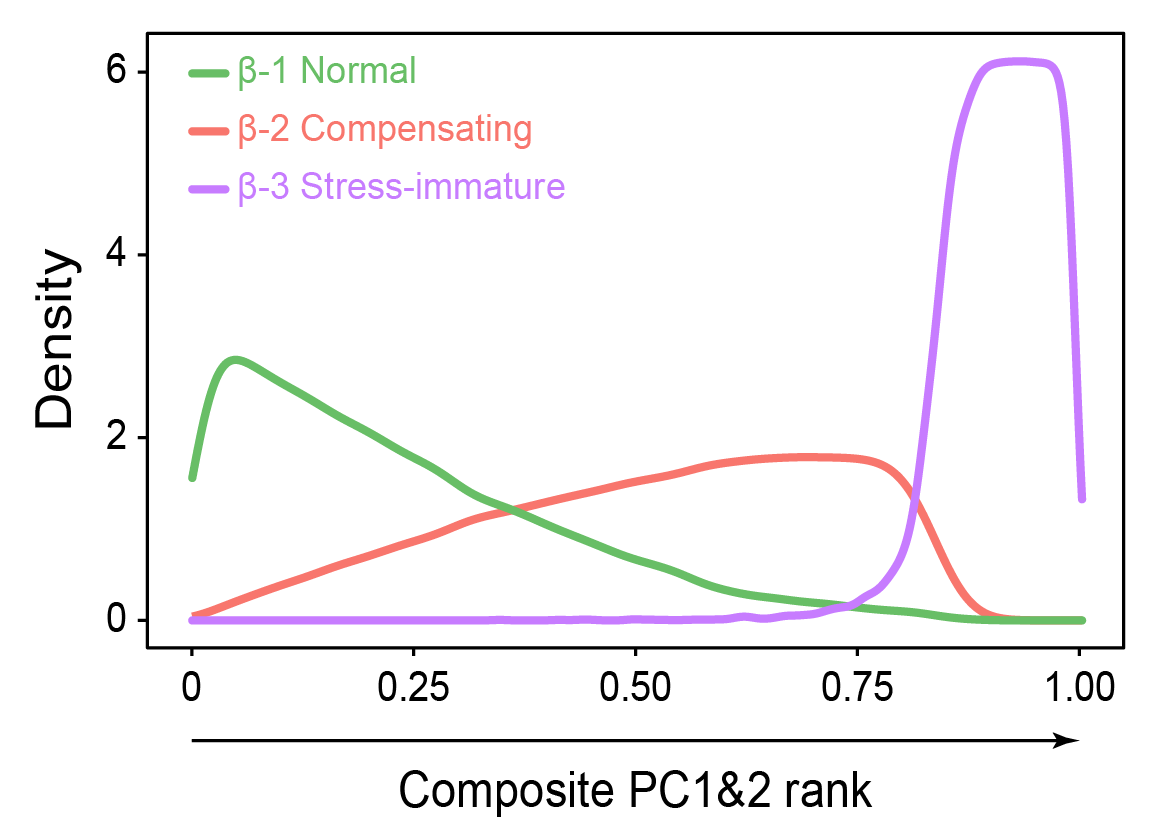
\includegraphics[width=10cm]{Chapter5/Fig/F3-6-04.png}
% \caption[Composite PC1 \& PC2]{}
% \label{fig:3-8}
% \end{wrapfigure}

\begin{figure}[t]
\centering
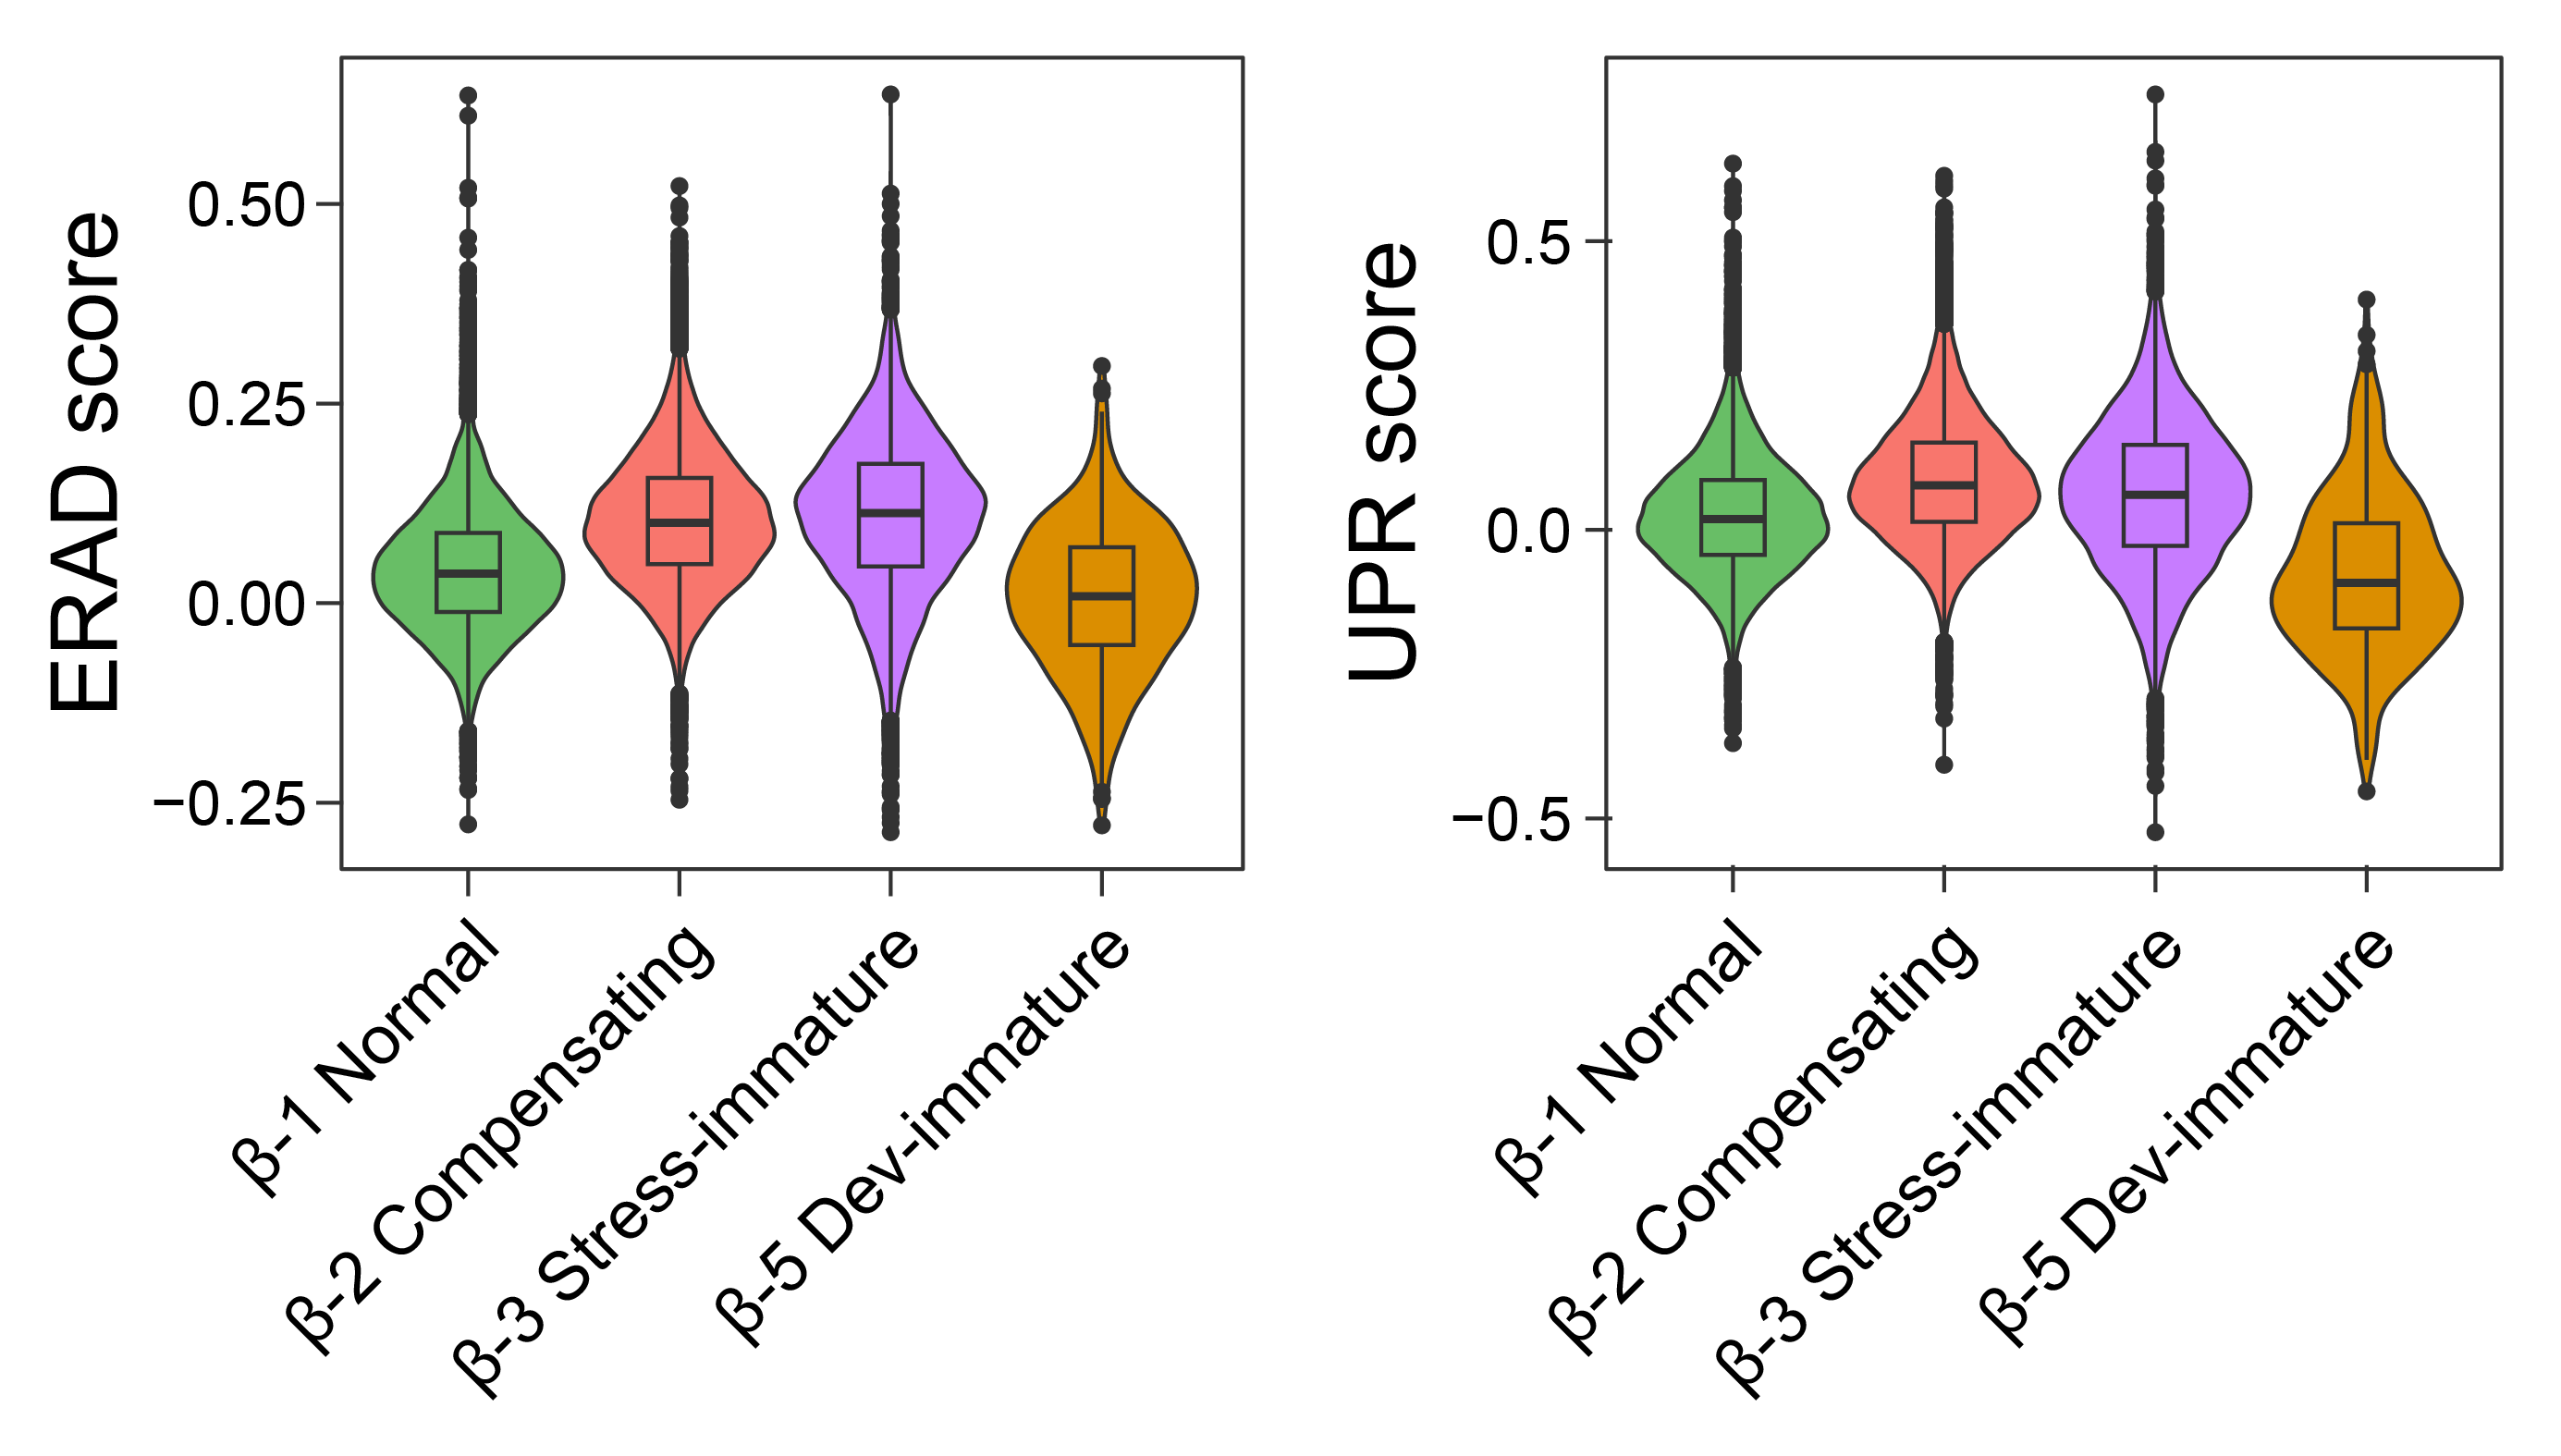
\includegraphics[width=\linewidth]{Chapter5/Fig/F3-22-01.png}
\caption[Enhanced \glsentryshort{erad} and \glsentryshort{upr} in response to increasing workloads in $\beta$-cells]{\textbf{Enhanced \gls{erad} and \gls{upr} in response to increasing workloads in $\beta$-cells.} Violin plots depicting the gene set score for \gls{erad} and \gls{upr} processes across the four indicated $\beta$-cell subsets. On the overlay box plots, the middle horizontal line represents the median, the box represents the inter-quartile range and the whiskers represent the minimum and maximum values.}
\label{fig:chp3_eradupr}
\end{figure}





\par Combining \gls{pc}1 and \gls{pc}2, we hypothesized that the three major $\beta$-cell subsets could be better represented along a composite axis that encompassed a degree of maturity (\gls{pc}1) and a degree of workload (\gls{pc}2) \textbf{(\autoref{fig:chp3_pca2}; \autoref{fig:app_chp3_pc12};} see \hyperref[subsubsec:met_chp3_pca]{\textbf{Methods}}\textbf{)}. Along this Maturity-Workload axes, the $\beta$-1 normal subset progressively switched to $\beta$-2 compensating subset, therefore indicating that $\beta$-1 and $\beta$-2 could be continuous phenotypes as opposed to two discrete subsets. The $\beta$-2 compensating subset exhibited signatures of increased workload but retained $\beta$-cell identity. The $\beta$-3 stress-immature subset exhibited increased workload and loss of mature identity in response to increased insulin demand, which distinguished this subset which was associated with the decompensation.\\

% \mysidecaption{0.4}{%, resulting in hyperglycemic phenotypes.\\
% \captionof{figure}[$\beta$-cell dysfunction corresponds to increased workload concomitant with loss of maturation]{\textbf{$\beta$-cell dysfunction corresponds to increased workload concomitant with loss of maturation.} Density plot depicting the distribution of the three major $\beta$-cell subsets as curves along normalized composite axis of \gls{pc}1 and \gls{pc}2.}
% {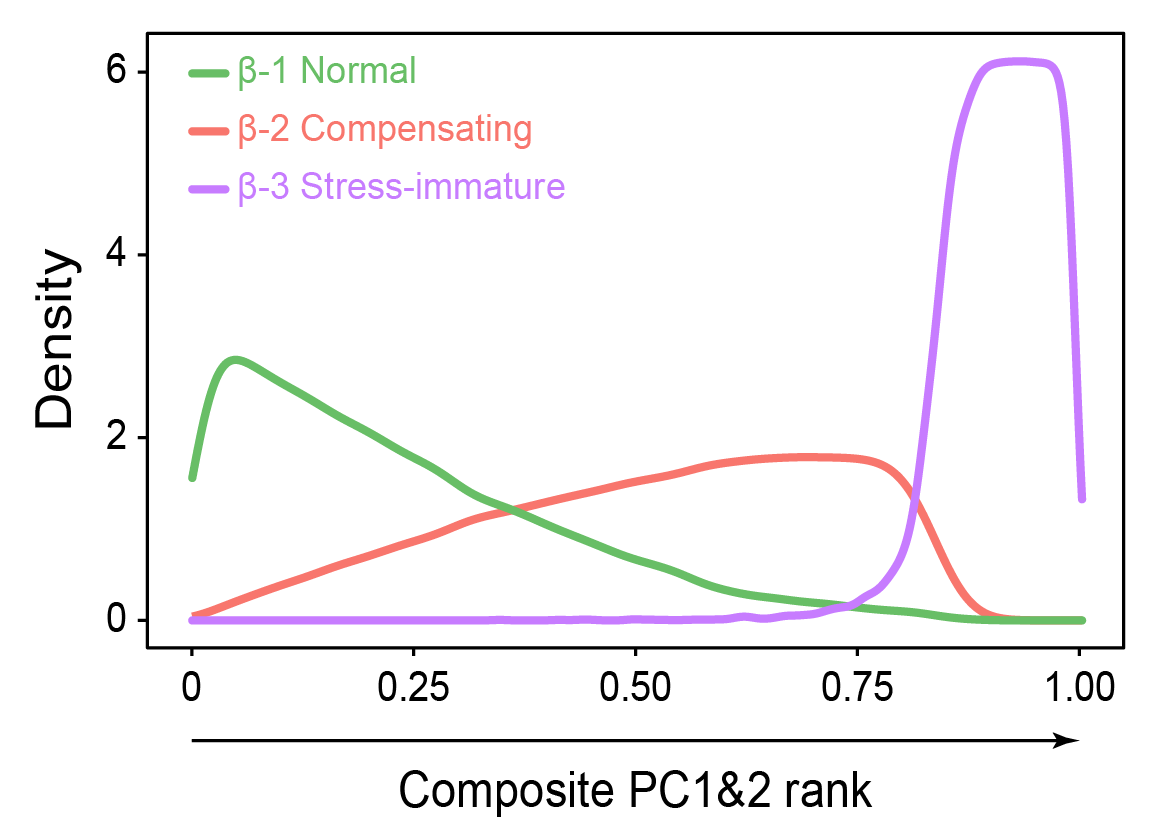
\includegraphics[width=9cm,height=9cm,keepaspectratio]{Chapter5/Fig/F3-6-04.png}}[H]%


\begin{wrapfigure}{r}{0.5\textwidth}
\vspace{-20pt}
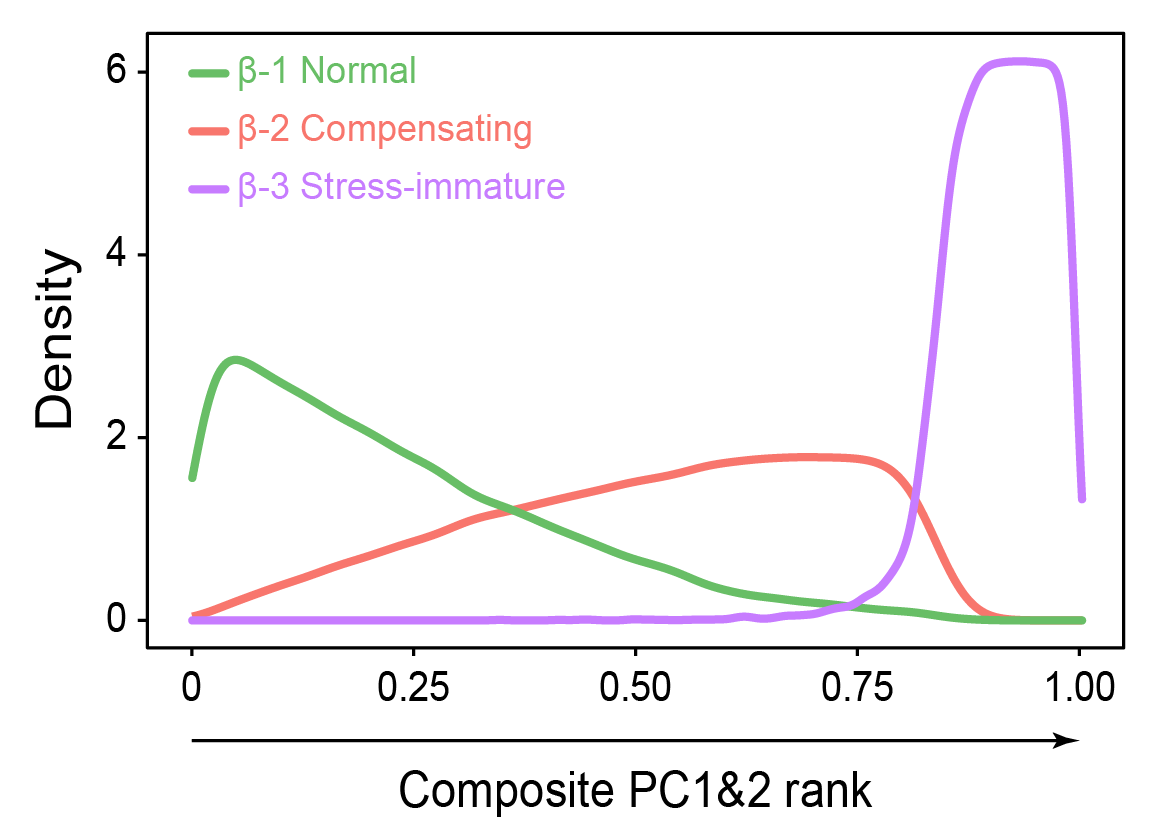
\includegraphics[width=7.5cm]{Chapter5/Fig/F3-6-04.png}
\caption[$\beta$-cell dysfunction corresponds to increased workload and loss of maturation]{\textbf{$\beta$-cell dysfunction corresponds to increased workload concomitant with loss of maturation.}  Density plot depicting the distribution of the three major $\beta$-cell subsets as curves along rank normalized composite axes of \gls{pc}1 and \gls{pc}2.}
\label{fig:chp3_pca2}
\vspace{-15pt}
\end{wrapfigure}

\par In summary, \gls{pca} delineated the three principal $\beta$-cell subsets and highlighted their dynamic responses to increased workload under various stresses. The distinctions and overlaps between the first two \glspl{pc}, the Maturity-Workload axes, suggest that normal and compensating $\beta$-cell subsets exist along this continumm and the stressed $\beta$-cell subset appears discrete from the other two major subsets. This underscores the complexity of $\beta$-cell identity and response under \gls{t2d} conditions.  

%\clearpage

\section[\glsentryshort{grn}s underlying the transcriptional heterogeneity of $\beta$-cell subsets]{Gene regulatory networks underlying the transcriptional\\heterogeneity of $\beta$-cell subsets}
\label{sec:chp3_betaGRN}


\begin{wrapfigure}{l}{0.6\textwidth}
\vspace{-30pt}
%\centering
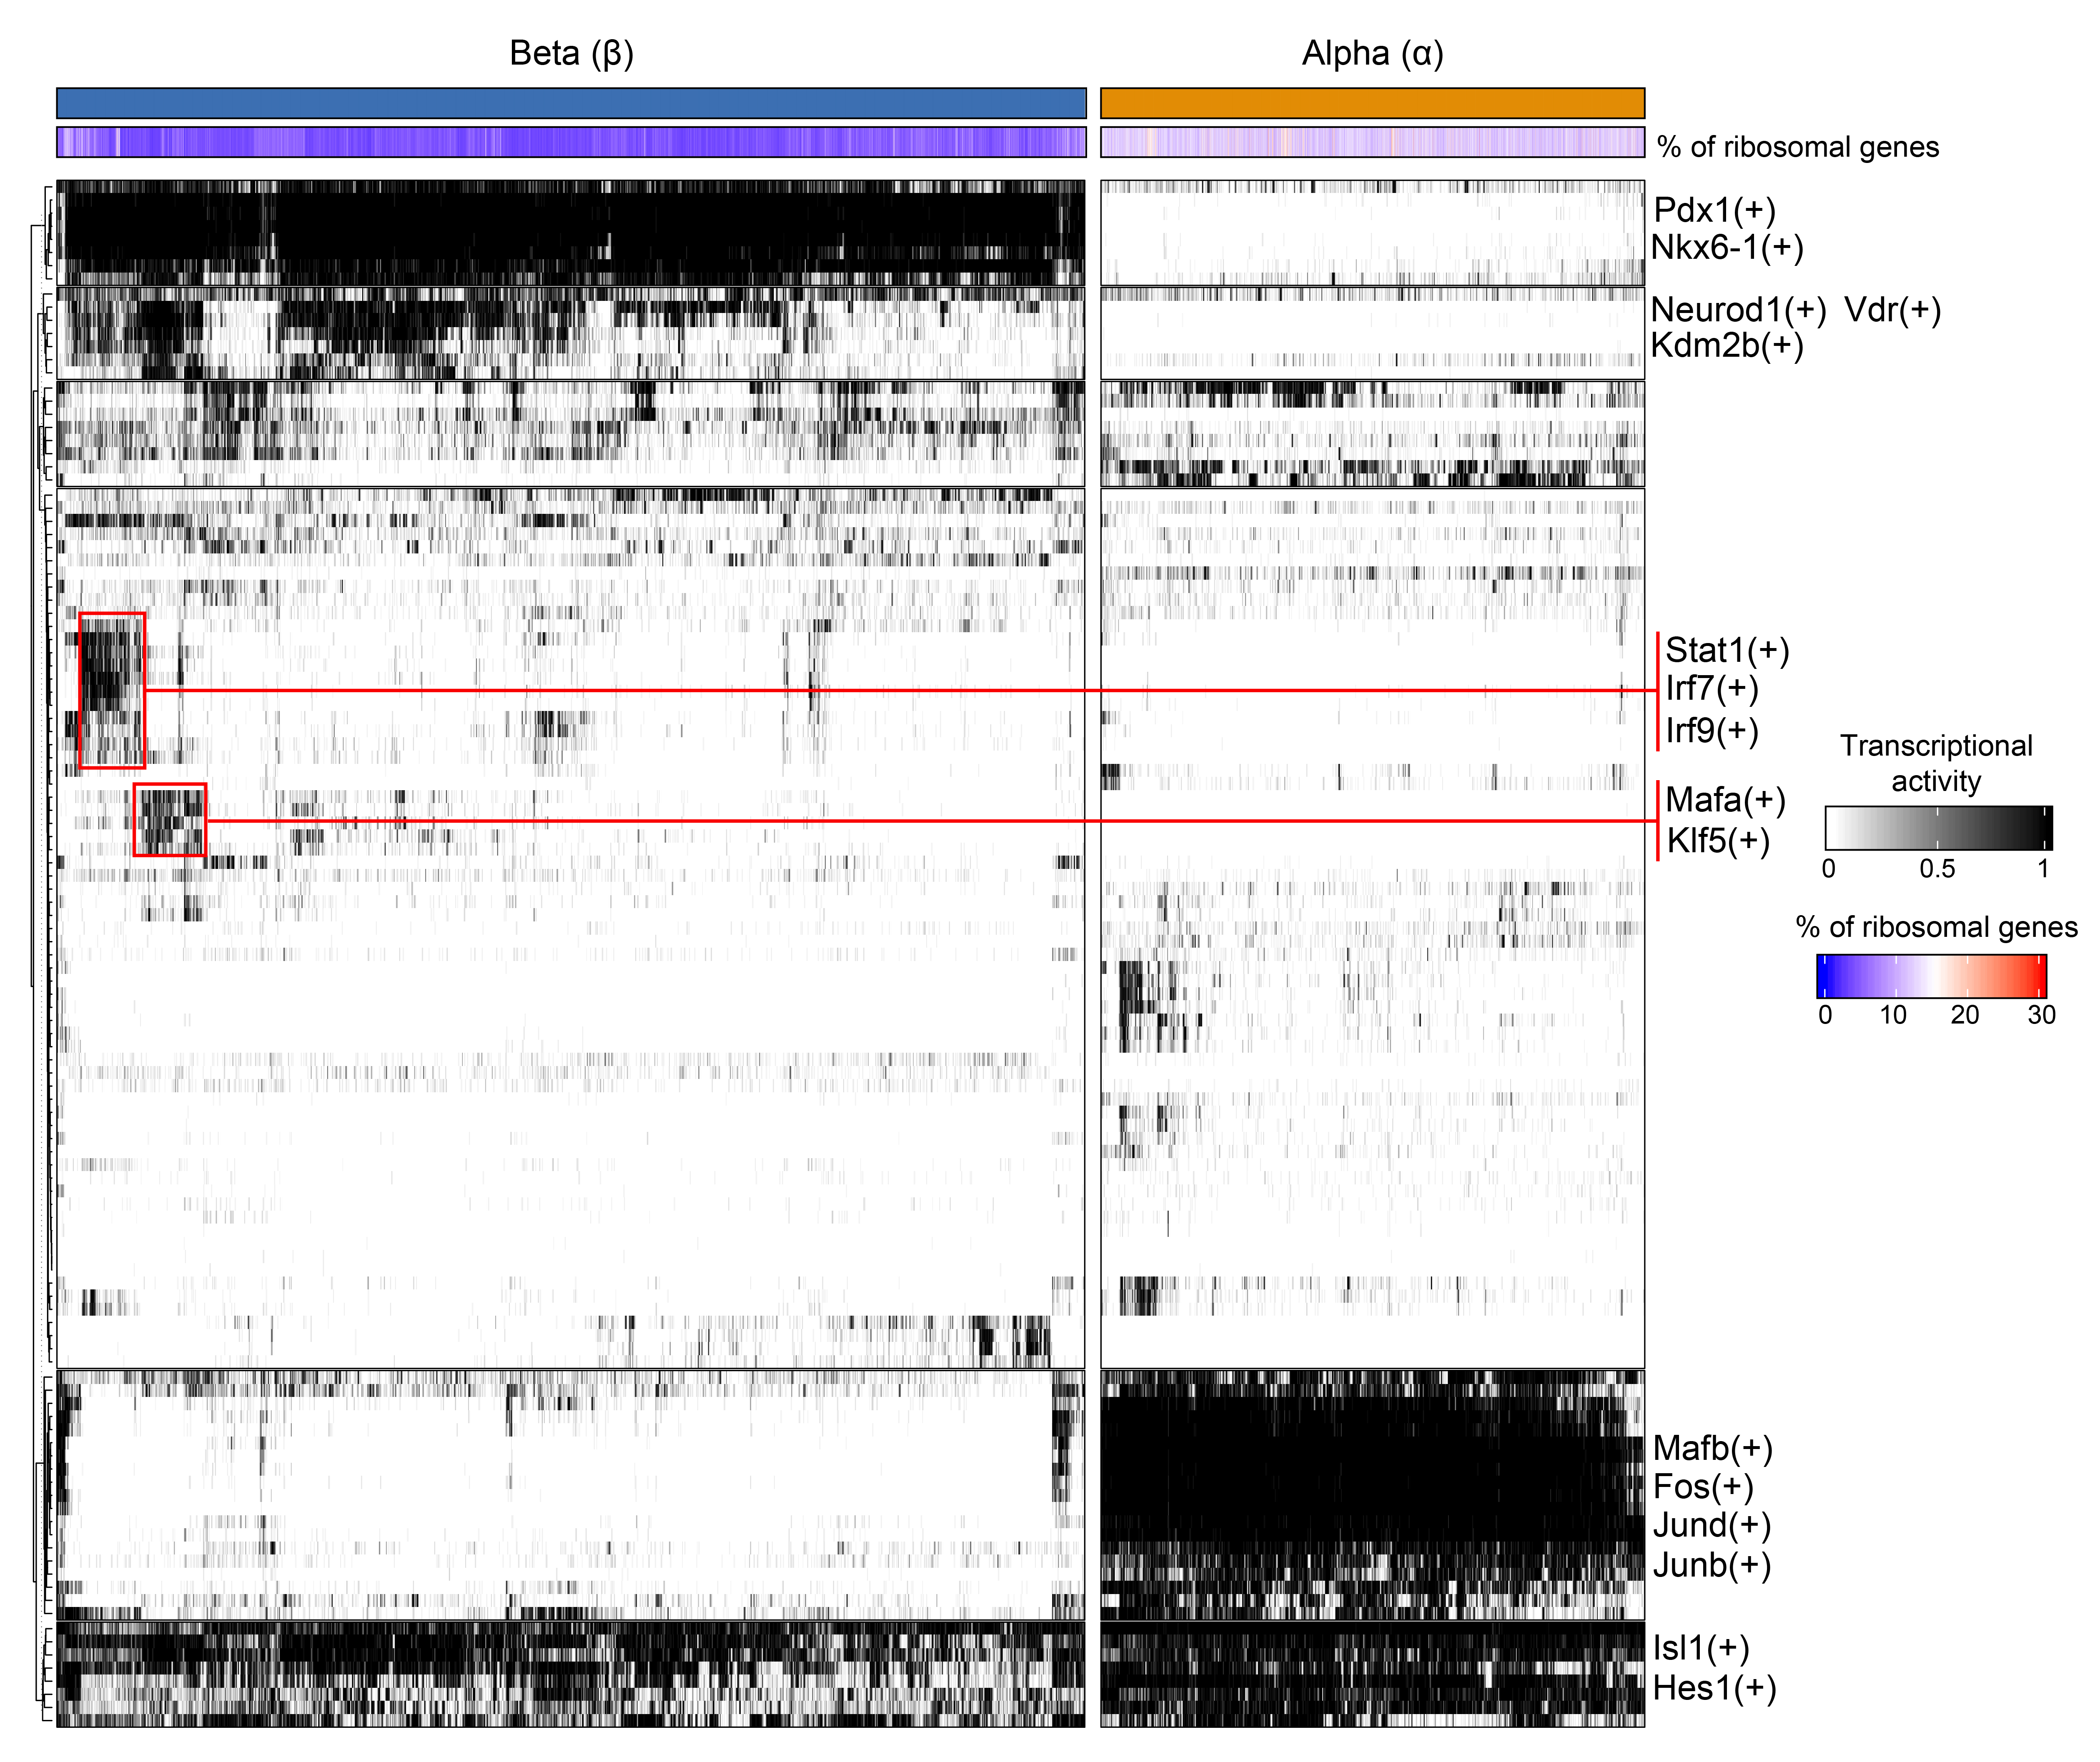
\includegraphics[width=8.5cm]{Chapter5/Fig/F3-11-01.png}
%\vspace{10pt}
\caption[Identification of cell-type specific regulons]{\textbf{Identification of cell-type specific regulons.} Heatmap depicting the binarized area under the curve (AUC) scores, representing the transcriptional activity of regulons across $\alpha$-cells and $\beta$-cells. Regulons shown in black are considered "ON", while regulons in white are considered "OFF". The top color bar depicts the grouping by cell types. The bottom color bar depicts the percentage of ribosomal (\textit{Rpl\textsuperscript{*}} and \textit{Rps\textsuperscript{*}}) genes for all cells.}
\vspace{-40pt}
\label{fig:chp3_scenic_alphabeta}
% \vspace{-5pt}
\end{wrapfigure}

Unraveling the complex web of \glspl{grn} is fundamental to decoding the complex regulatory mechanisms that govern cellular response to environmental cues. The development and maturation of $\beta$-cells is tightly regulated by the coordinated activity of several key \glspl{tf} (Pdx1, Mafa and Nkx6-1) that target several genes in order to maintain normal $\beta$-cell identity and function. However, very little is known about how \glspl{tf} in $\beta$-cells are affected in response to increasing workload, and how they govern state transitions. Therefore, to understand the molecular mechanisms that underlie these transcriptional differences, we performed \gls{grn} analysis using \textit{pySCENIC} to infer \gls{tf} activity and infer \gls{tf}-specific \glspl{grn} \textbf{\cite{kumar_inference_2021}}.\\

%A description of the workflow for \gls{grn} inference using the SCENINC workflow can be found in \hyperref[sec:scrna_analysis_grn]{Section 1.5.6}.\\

\par We identified \glspl{grn} within two islet cell types in our data: Alpha ($\alpha$) and Beta ($\beta$). We extracted all cells annotated as Alpha ($\alpha$) in the full integrated data \textbf{(\autoref{fig:chp3_fulldata} A)} and re-integrated this subset with the non-proliferating $\beta$-cells, which included all $\beta$-cell subsets except $\beta$-4. We then applied \textit{pySCENIC} and identified $\alpha$-cell and $\beta$-cell specific regulons \textbf{(\autoref{fig:chp3_scenic_alphabeta};} see \hyperref[subsubsec:met_chp3_scenic]{\textbf{Methods}}\textbf{)}. A regulon is defined as a regulatory network that connects a \gls{tf} with its target genes. We identified Pdx1, Nkx6-1 and Mafa regulons in $\beta$-cells and the Mafb regulon in $\alpha$-cells. The Isl1 regulon was active in both cell types, and is regarded as a shared \gls{tf} regulator in the islet cell lineage \textbf{\cite{juhl_mouse_2008}}, controlling pancreatic $\alpha$-cell fate and $\beta$-cell maturation \textbf{\cite{bohuslavova_isl1_2023}}. In addition, the \gls{tf} Hes1, a downstream target of \textit{Notch} \textbf{\cite{hashemitabar_redefining_2019}}, was also active in both the cell types.\\



%\clearpage to the Alpha ($\alpha$)-Beta ($\beta$) re-integrated subset in order to identify
\par In $\beta$-cells, we identified 124 regulons across the five non-proliferating subsets. \glspl{tf} often work in coordination to regulate gene expression levels. Therefore, to determine the degree of \gls{tf} activity coordination in the $\beta$-cells, we computed \gls{csi} on the basis of pairwise comparisons of regulon activity patterns, and identified five modules with varying number of regulons \textbf{(\autoref{fig:chp3_scenic_betaonly} A; \autoref{tab:app_chp3_regulons};} see \hyperref[subsubsec:met_chp3_scenic]{\textbf{Methods}}\textbf{)}. We also visualized the transcriptional \gls{grn} underlying the non-proliferating $\beta$-cells by using the top 1\% of the reported \gls{tf}-target associations \textbf{(\autoref{fig:chp3_scenic_betaonly} B)}.

\vspace{-10pt}
\begin{figure}[H]
\centering
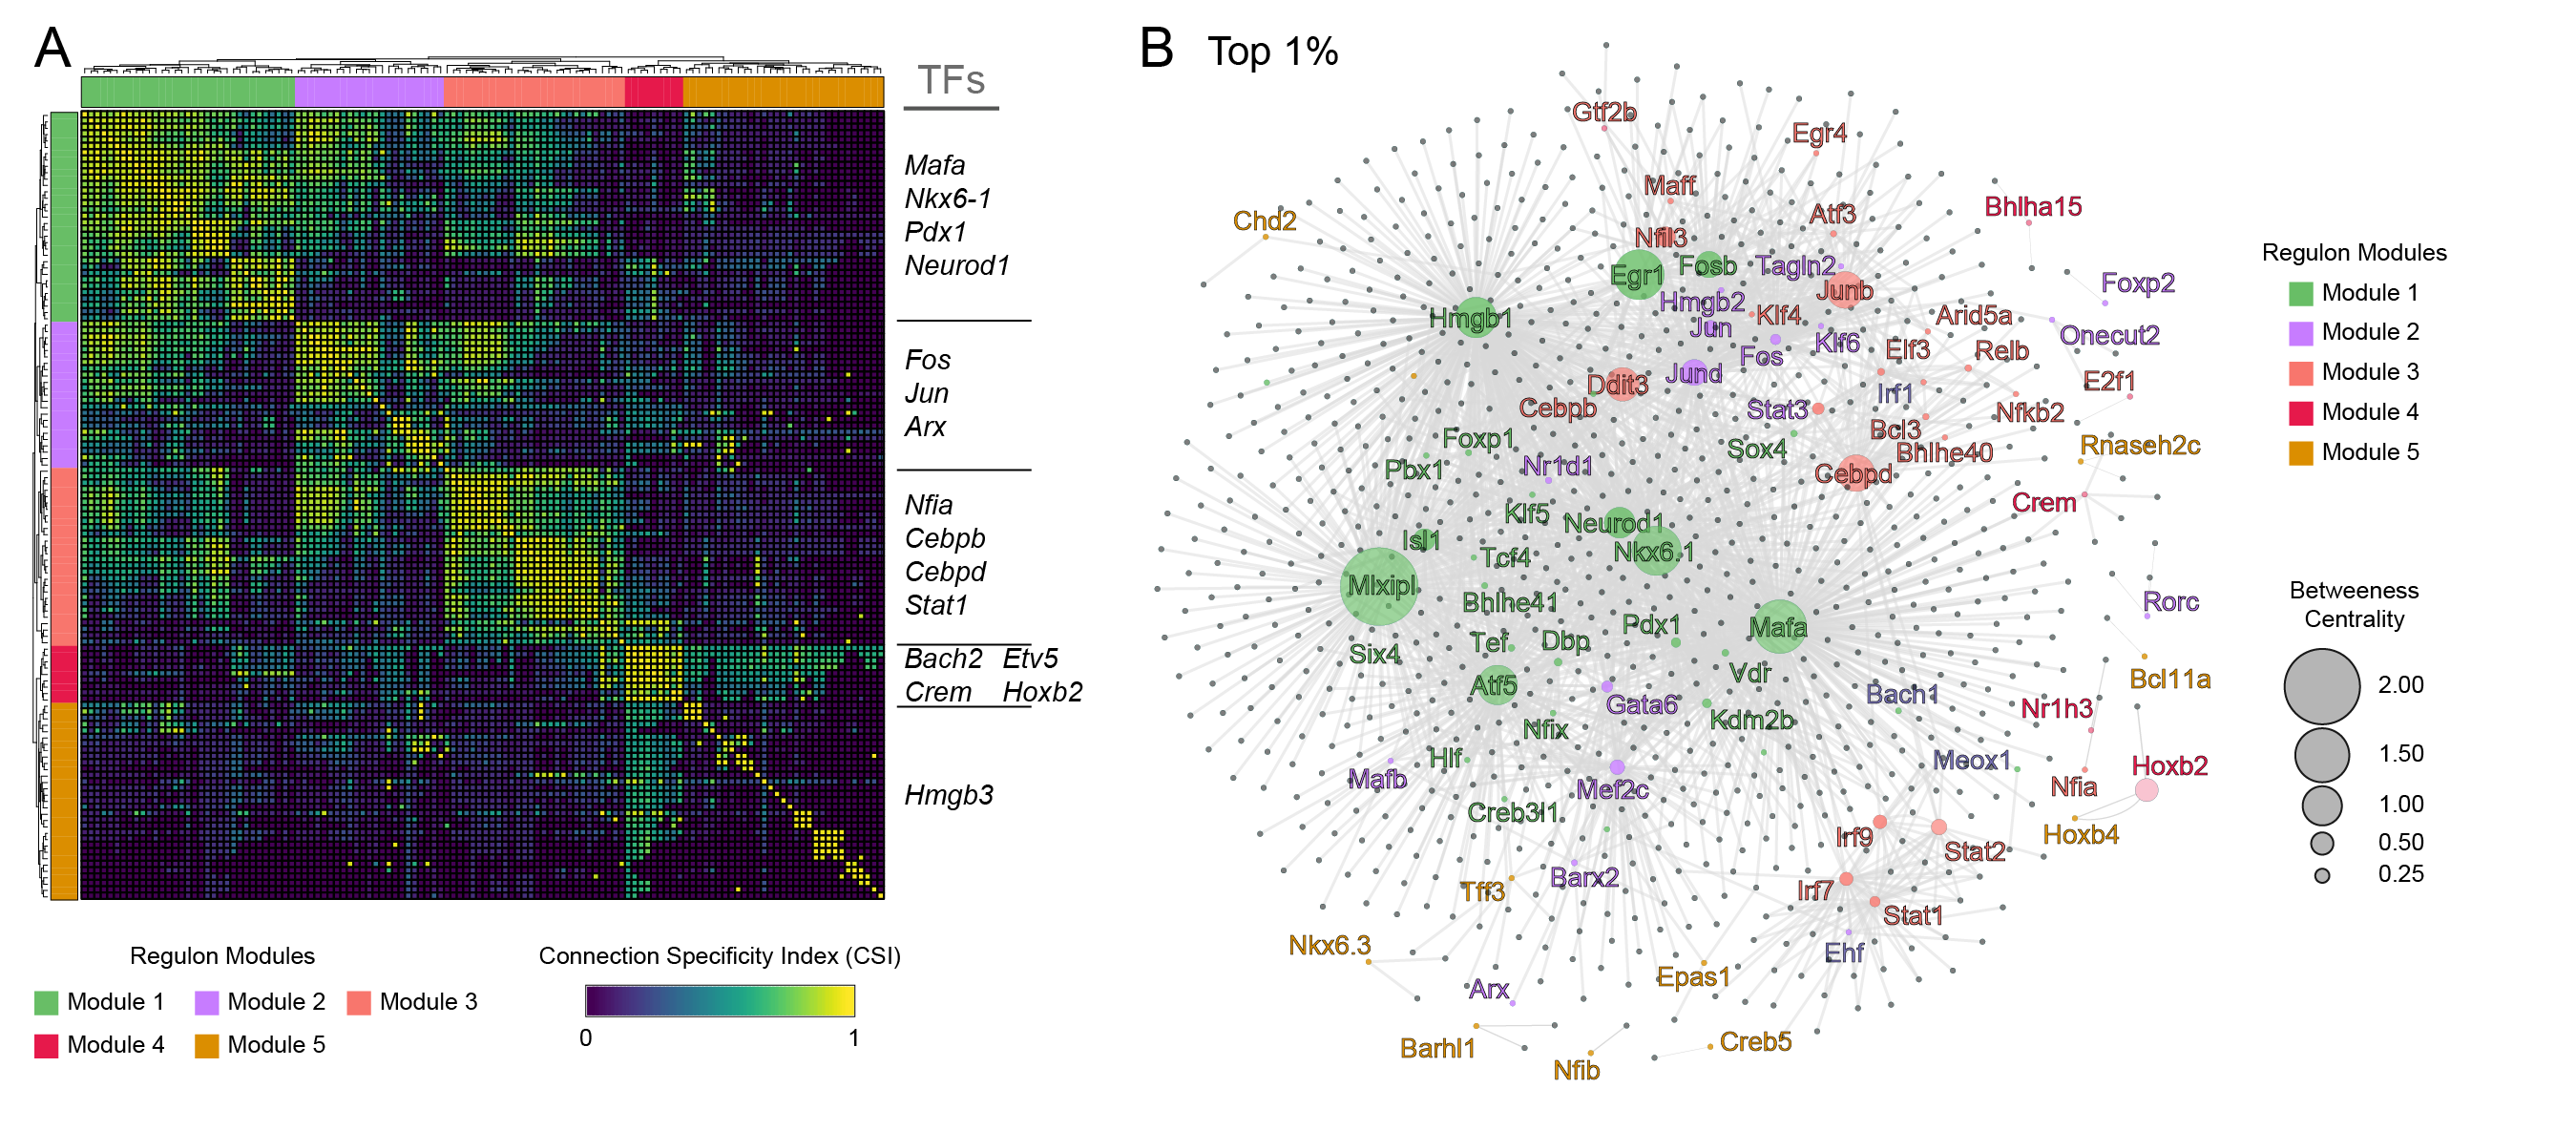
\includegraphics[width=\linewidth]{Chapter5/Fig/F3-10-02.png}
\caption[Identification of $\beta$-cell specific \glsentryshort{grn} and regulon modules]{\textbf{Identification of $\beta$-cell specific \gls{grn} and regulon modules.} \textbf{(A)} Hierarchical clustering of non-proliferating $\beta$-cell-specific regulons using \gls{csi} as a distance measure and yielded five modules. \textbf{(B)} \gls{grn} formed by \glspl{tf} identified using \textit{pySCENIC} in non-proliferating $\beta$-cells. \glspl{tf} are colored according to their modules while target genes are depicted in gray. Lines connecting the nodes represent the importance metric between \gls{tf}-gene pairs, where thicker edges indicate stronger \gls{tf}-target relationship. Node size represents the betweenness centrality, computed within Cytoscape, and reports on the influence of a given \gls{tf} within the network.}
\label{fig:chp3_scenic_betaonly}
\end{figure}




% \begin{figure}[t]
% \centering
% 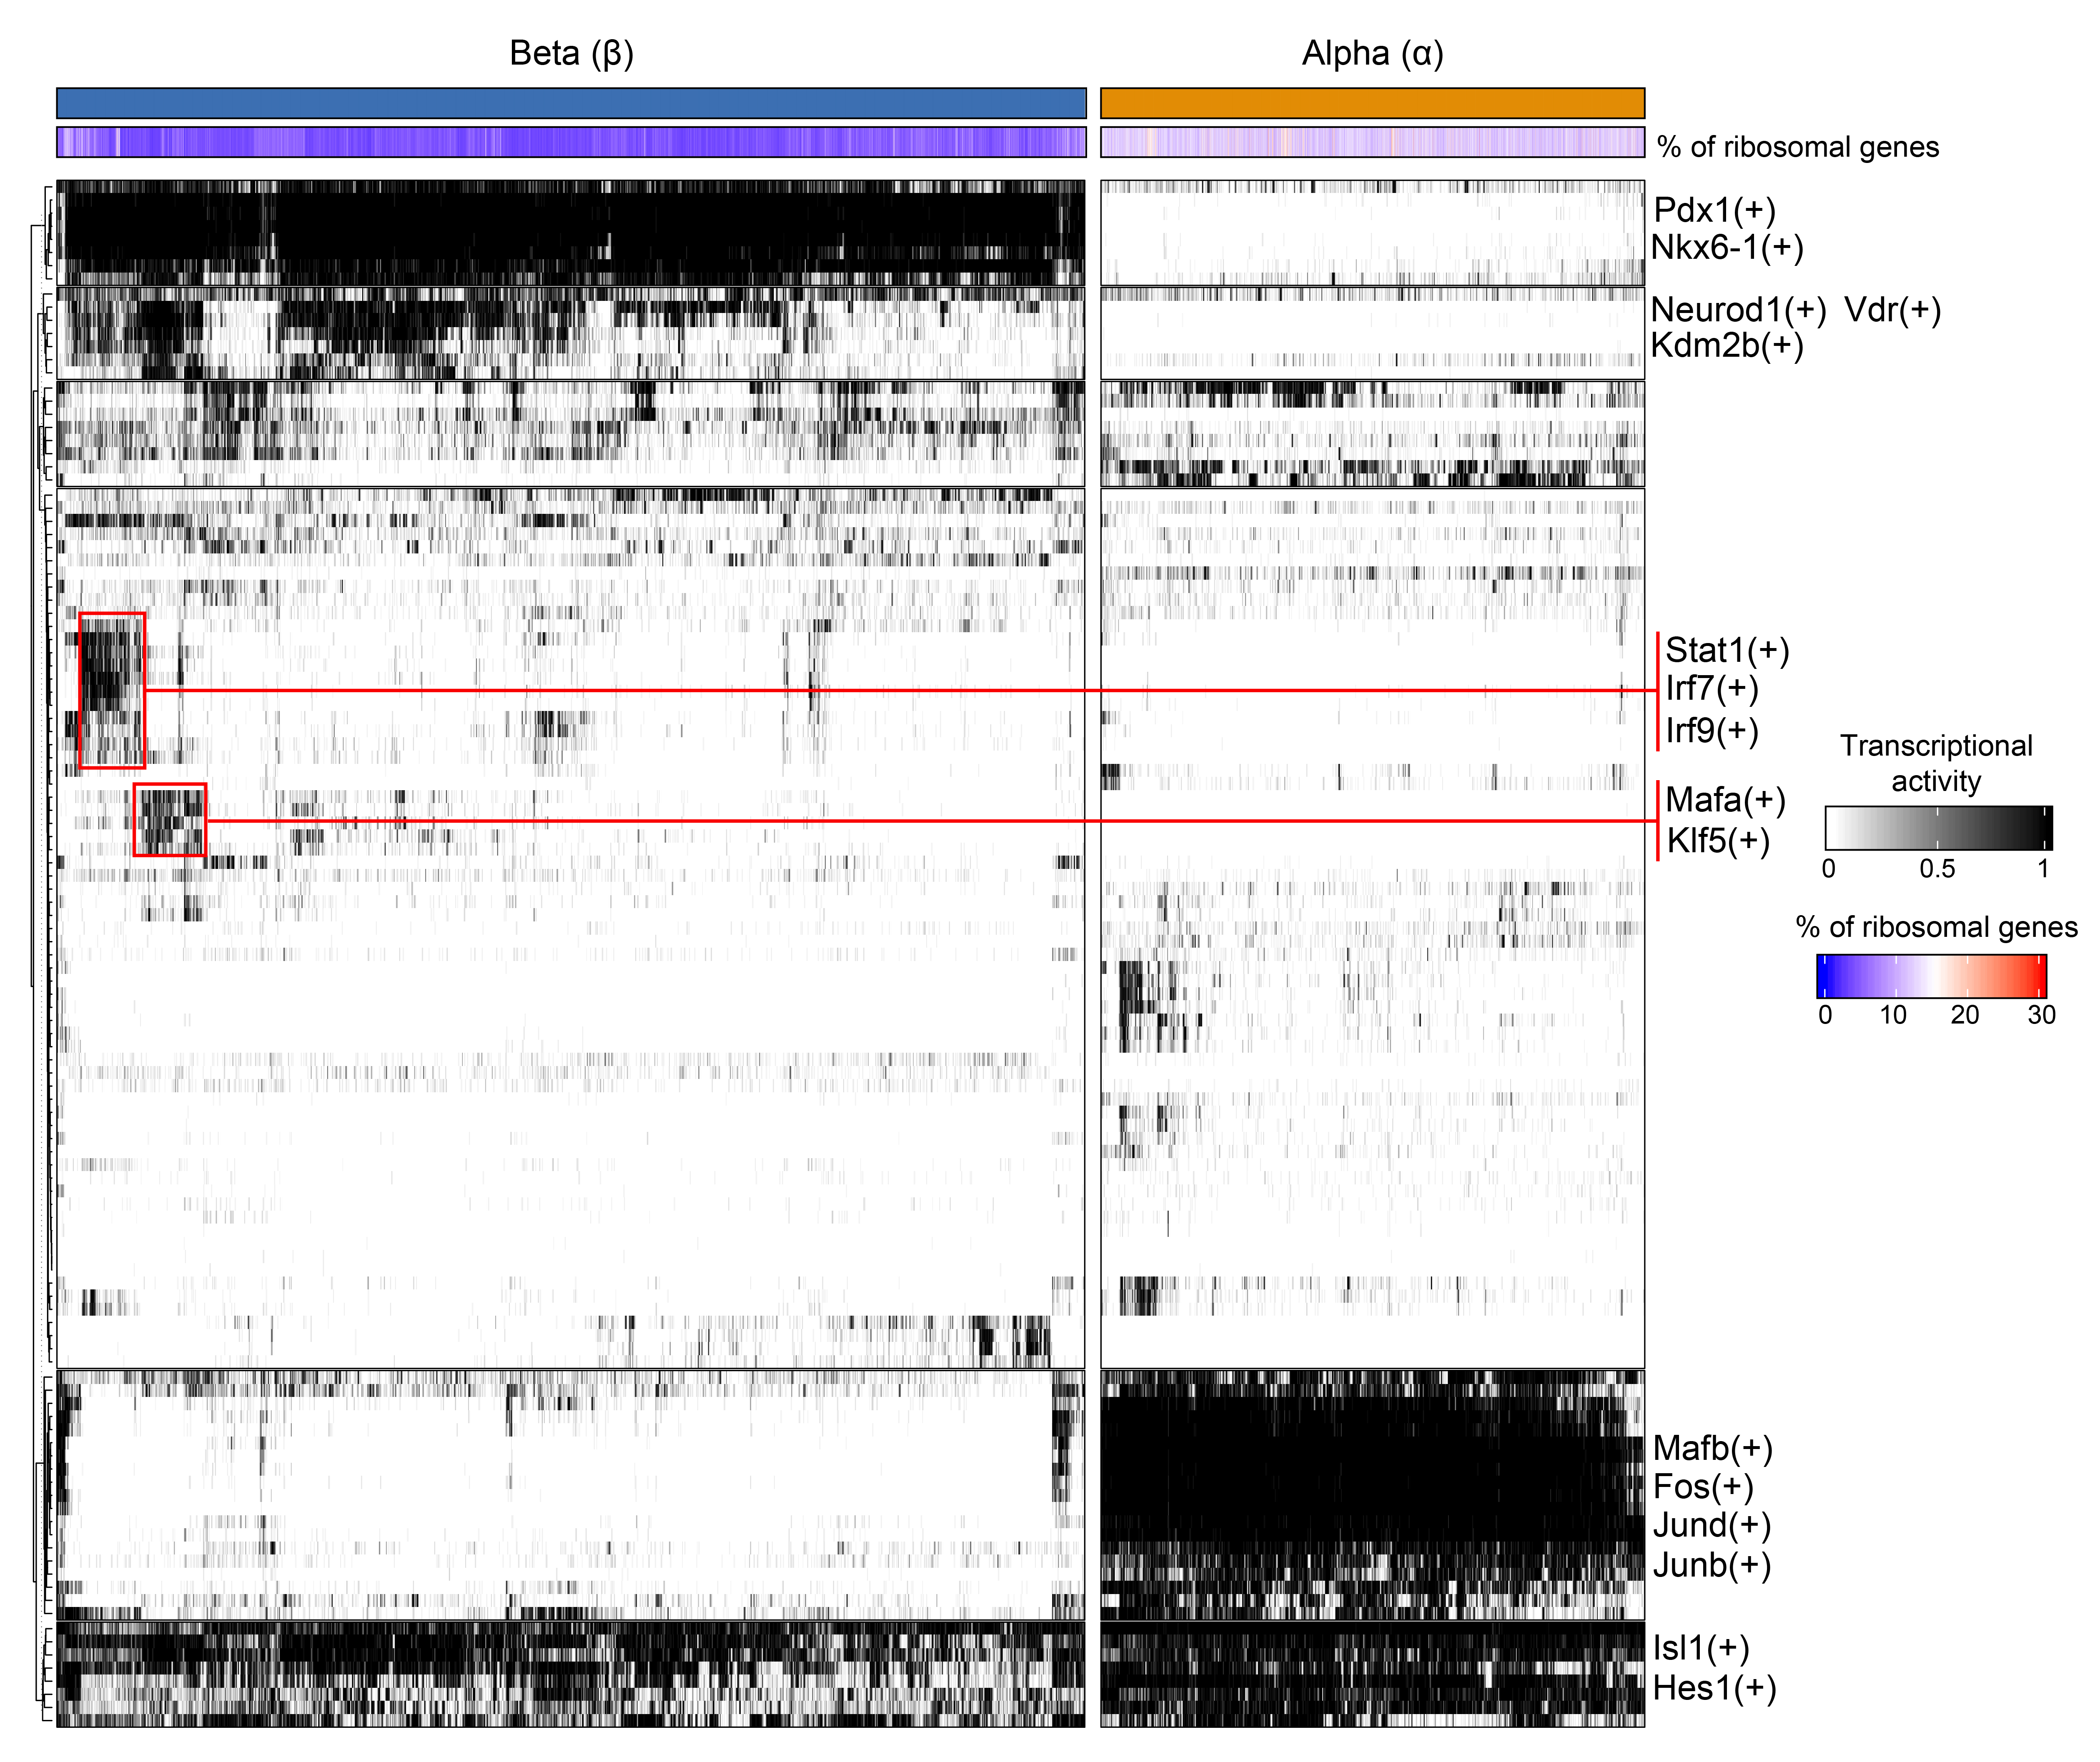
\includegraphics[width=12cm]{Chapter5/Fig/F3-11-01.png}
% \caption[Identification of cell-type specific regulons]{\textbf{Identification of cell-type specific regulons.} Heatmap depicting the binarized \gls{auc} scores, representing the transcriptional activity of regulons across all the cells. Regulons shown in black are considered "ON", while regulons in white are considered "OFF". Several characteristic regulons are highlighted and denoted with `(+)' after the \gls{tf}. The top color bar depicts the cell-type annotation and the bottom color bar depicts the percentage of ribosomal genes in each cell.}
% \label{fig:chp3_scenic_alphabeta}
% \end{figure}

\par Overall, the observed regulon activity patterns across the various $\beta$-cell subsets \textbf{(\autoref{fig:app_chp3_scenic_betasubsets})} matched the activity patterns in response to each intervention for all studies \textbf{(\autoref{fig:app_chp3_scenic_studies})}. This alignment further supported the robustness of the $\beta$-cell subset classification based on cellular processes characteristic of each subset. Critical \gls{tf} regulons associated with $\beta$-cell development and function (Neurod1, Mafa, Nkx6-1 and Pdx1) clustered together in Module 1 \textbf{(\autoref{fig:chp3_scenic_betaonly} A; \autoref{fig:chp3_scenic_betasubsets}; \autoref{tab:app_chp3_regulons})} with the Neurod1 regulon depicting quantitatively higher activity in the $\beta$-1 normal subset compared to the $\beta$-2 compensating and $\beta$-3 stress-immature subsets \textbf{(\autoref{fig:chp3_scenic_betasubsets})}. In addition, the $\beta$-1 normal subset also showed higher activity for Nfia regulon \textbf{(\autoref{fig:chp3_scenic_betasubsets})}, which was part of Module 3 and is known regulate endocrine fate induction \textbf{\cite{scavuzzo_pancreatic_2018}} and regulates pancreatic physiology through insulin granule recruitment and docking \textbf{\cite{scavuzzo_nfia_2019}}. Within Module 1, We were also able to identify a novel candidate regulator, lysine (K)-specific demethylase 2B (Kdm2b), with regulon activity similar to that of the Neurod1 regulon \textbf{(\autoref{fig:chp3_scenic_betasubsets})}. Examining the target genes of Kdm2b, we identified important genes relating to  $\beta$-cell function (\textit{Mafa, Atp2a2}), thereby suggesting some important role for this histone demethylase in $\beta$-cell function. Furthermore, the activity of this regulon was down-regulated in all stress-associated models compared to their corresponding controls \textbf{(\autoref{fig:app_chp3_scenic_studies})}, hinting at some role for this histone demethylase in regulating stress responses in $\beta$-cells.


\begin{figure}[H]
\centering
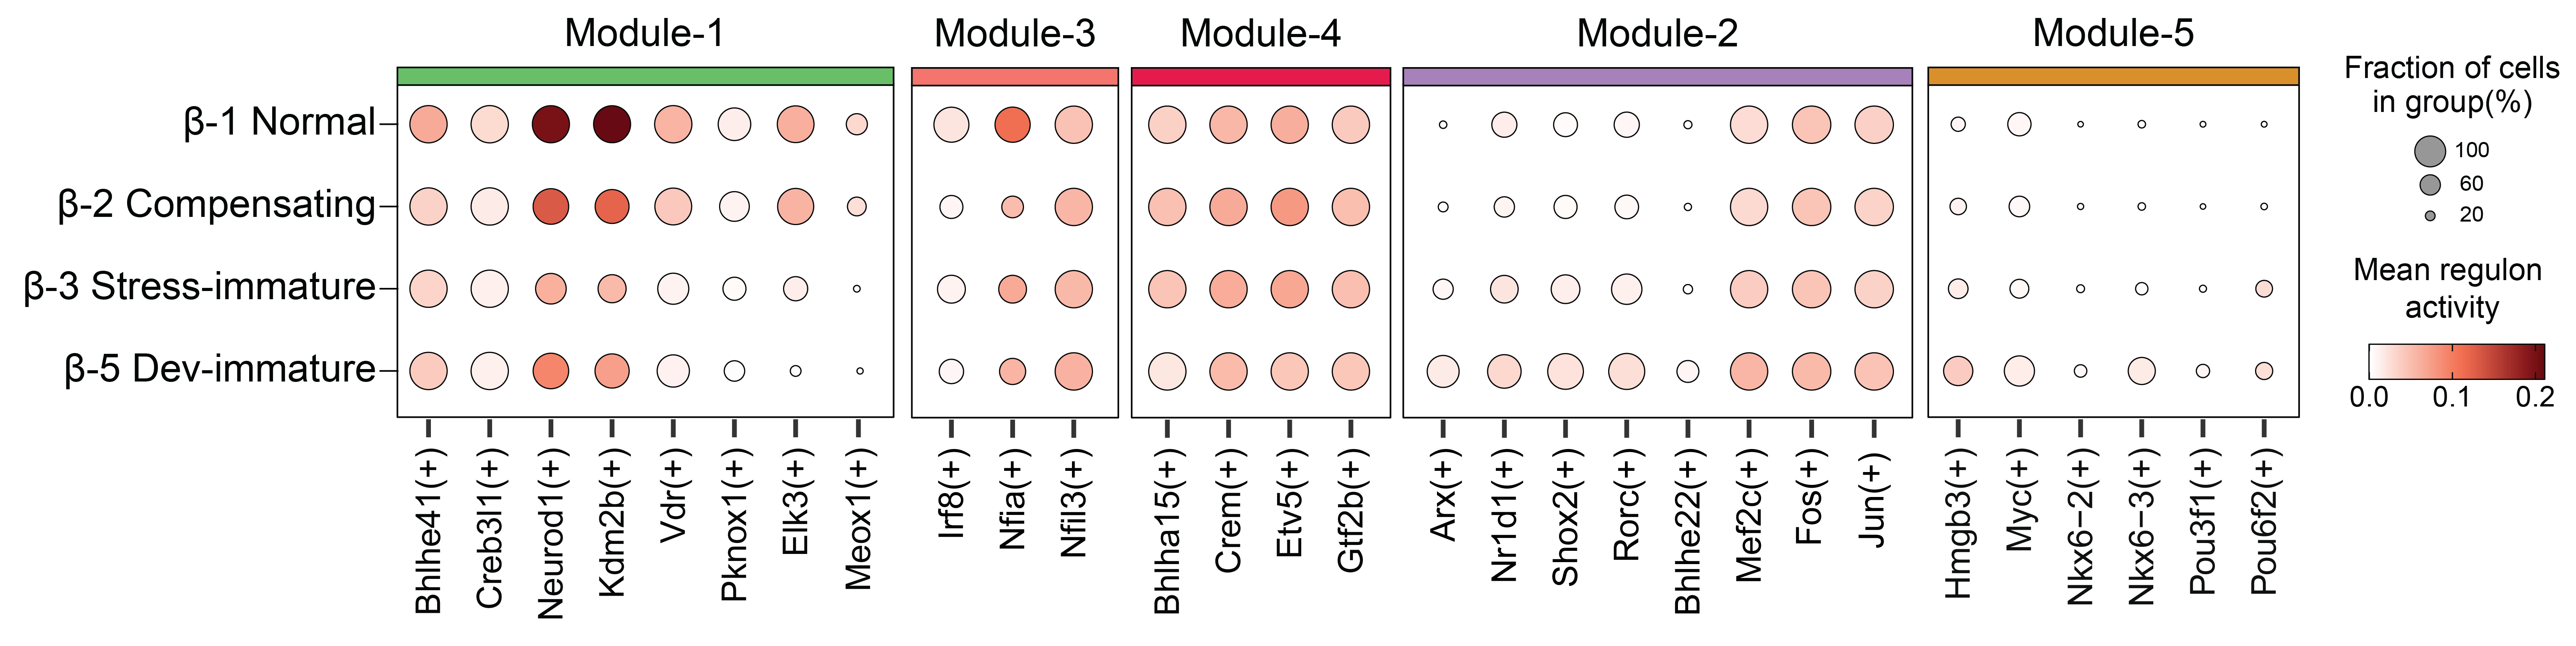
\includegraphics[width=\linewidth]{Chapter5/Fig/F3-12-v2-02.png}
\caption[Activity of \glsentryshort{tf}-regulons complements $\beta$-cell subset annotations]{\textbf{Activity of \gls{tf}-regulons complements $\beta$-cell subset annotations.} Dot plot depicting the mean activity of the indicated regulons across $\beta$-1, $\beta$-2, $\beta$-3 and $\beta$-5 subsets. The regulons are grouped by modules identified based on hierarchical clustering of the regulons using \gls{csi} as a distance measure. The color of the dots indicate the mean activity and the size of the dots correspond to the fraction of cells in which the regulon is active.}
\label{fig:chp3_scenic_betasubsets}
\end{figure}


% \textit{Kdm2b} (\textit{Ndy1}) was identified as a physiological inhibitor of senescence in fibroblasts 

% Therefore, \textit{Kdm2b} might regulate stress responses such as senescence, which has been implicated in both, \gls{t1d} and \gls{t2d}.\\  The observed lower activity could also result from the overall decrease in  $\beta$-cell numbers after ablation by \gls{stz}

\par The \textit{pySCENIC} analysis also revealed that the down-regulation in the activity of Module 1 regulons such as Vdr, Pknox1, Elk3 and Meox1 was associated with increasing $\beta$-cell workload resulting in $\beta$-cell dysfunction \textbf{(\autoref{fig:chp3_scenic_betasubsets})}. The regulon activity of mesenchyme homeobox 1 (Meox1) was also considerably reduced in all workload-associated models except for the feeding intervention \textbf{(\autoref{fig:app_chp3_scenic_studies})}. Regarding the vitamin D receptor (Vdr), a recent study demonstrated that Vdr expression was modulated by glucose in healthy islets and was down-regulated in islets from both, \gls{t1d} and \gls{t2d} mouse models \textbf{\cite{morro_vitamin_2020}}. Furthermore, $\beta$-cell specific over-expression of \textit{Vdr} in transgenic mice conferred protection against \gls{stz}-induced diabetes \textbf{\cite{morro_vitamin_2020}}. Mirroring these observations, the regulon activity of Vdr was lower in the \gls{stz} treated mice included in this atlas compared to other hyperglycemic models \textbf{(\autoref{fig:app_chp3_scenic_studies})}. The ternary complex factors (TCFs) such as Elk1, Elk3 and Elk4, along with the \gls{tf} early growth response 1 (Egr1), regulate glucose homeostasis and pancreatic islet size, with one study depicting that the transcriptional repression of genes regulated by all TCF family of proteins played an important role in $\beta$-cells \textbf{\cite{lesch_ternary_2020}}. The motifs of several Elk proteins were also found to be enriched at feeding-regulated sites in the epigenome \textbf{\cite{wortham_nutrient_2023}}. Elk3 induces genes for cellular adaptation to hypoxia and regulates the stability of hypoxia-inducible factor HIF-1$\alpha$ \textbf{\cite{gross_ternary_2007,gross_ternary_2008}}, with hypoxia leading to $\beta$-cell dysfunction and impaired insulin secretion \textbf{\cite{tsuyama_hypoxia_2023}}. The observed down-regulation in the regulon activity of Elk3 in the $\beta$-3 stress-immature subset \textbf{(\autoref{fig:chp3_scenic_betasubsets})} suggests a potential role for this TCF in $\beta$-cell function.\\





% Elk3 in particular is involved in induction of genes involved in cellular adaptation to hypoxia and regulates the protein stability of hypoxia-inducible factor HIF-1$\alpha$ , with hypoxia causing $\beta$-cell dysfunction and impaired insulin secretion  


\par A striking observation from this analysis was the up-regulation in the regulon activity of the aristaless-related homeobox gene (Arx) in both $\beta$-3 stress-immature and $\beta$-5 dev-immature subsets \textbf{(\autoref{fig:chp3_scenic_betasubsets})}. The \gls{tf} Arx specifies the formation of pancreatic islet $\alpha$-cell during development, and the forced over-expression of Arx within pancreata has shown massive reductions in $\beta$-cell and $\delta$-cell numbers and increased $\alpha$-cell and PP-cell numbers \textbf{\cite{van_der_meulen_role_2015}}. The higher activity of Arx in $\beta$-3 subset compared to the $\beta$-1 normal or $\beta$-2 compensating subsets likely suggests the activation of a dedifferentiation like-program in response to increased workload in hyperglycemic and insulin-resistant models. Similar to Arx, we observed that the $\beta$-3 and the $\beta$-5 subsets depicted higher regulon activity of retinoic acid-related orphan receptor C (Rorc) \textbf{(\autoref{fig:chp3_scenic_betasubsets})}, which has been identified to associate with human islet dysfunction. Furthermore the silencing of RORC genes resulted in reduced expression of \textit{Ins1} and \textit{Ins2} at the transcriptomic level and therefore reduced insulin secretion in rat INS-1 cells \textbf{\cite{taneera_rorb_2019}}. The Arx and Rorc regulons were part of Module 2 which also consisted of activator protein 1 (AP-1) \gls{tf} complexes such as Fos and Jun regulons \textbf{(\autoref{fig:chp3_scenic_betasubsets})} which are involved in stress response and have been implicated in the regulation of $\beta$-cell function, particularly under conditions of metabolic stress or diabetes \textbf{\cite{bahrami_gene_2016,backes_regulation_2021}}.\\


% \begin{figure}[t]
% \centering
% 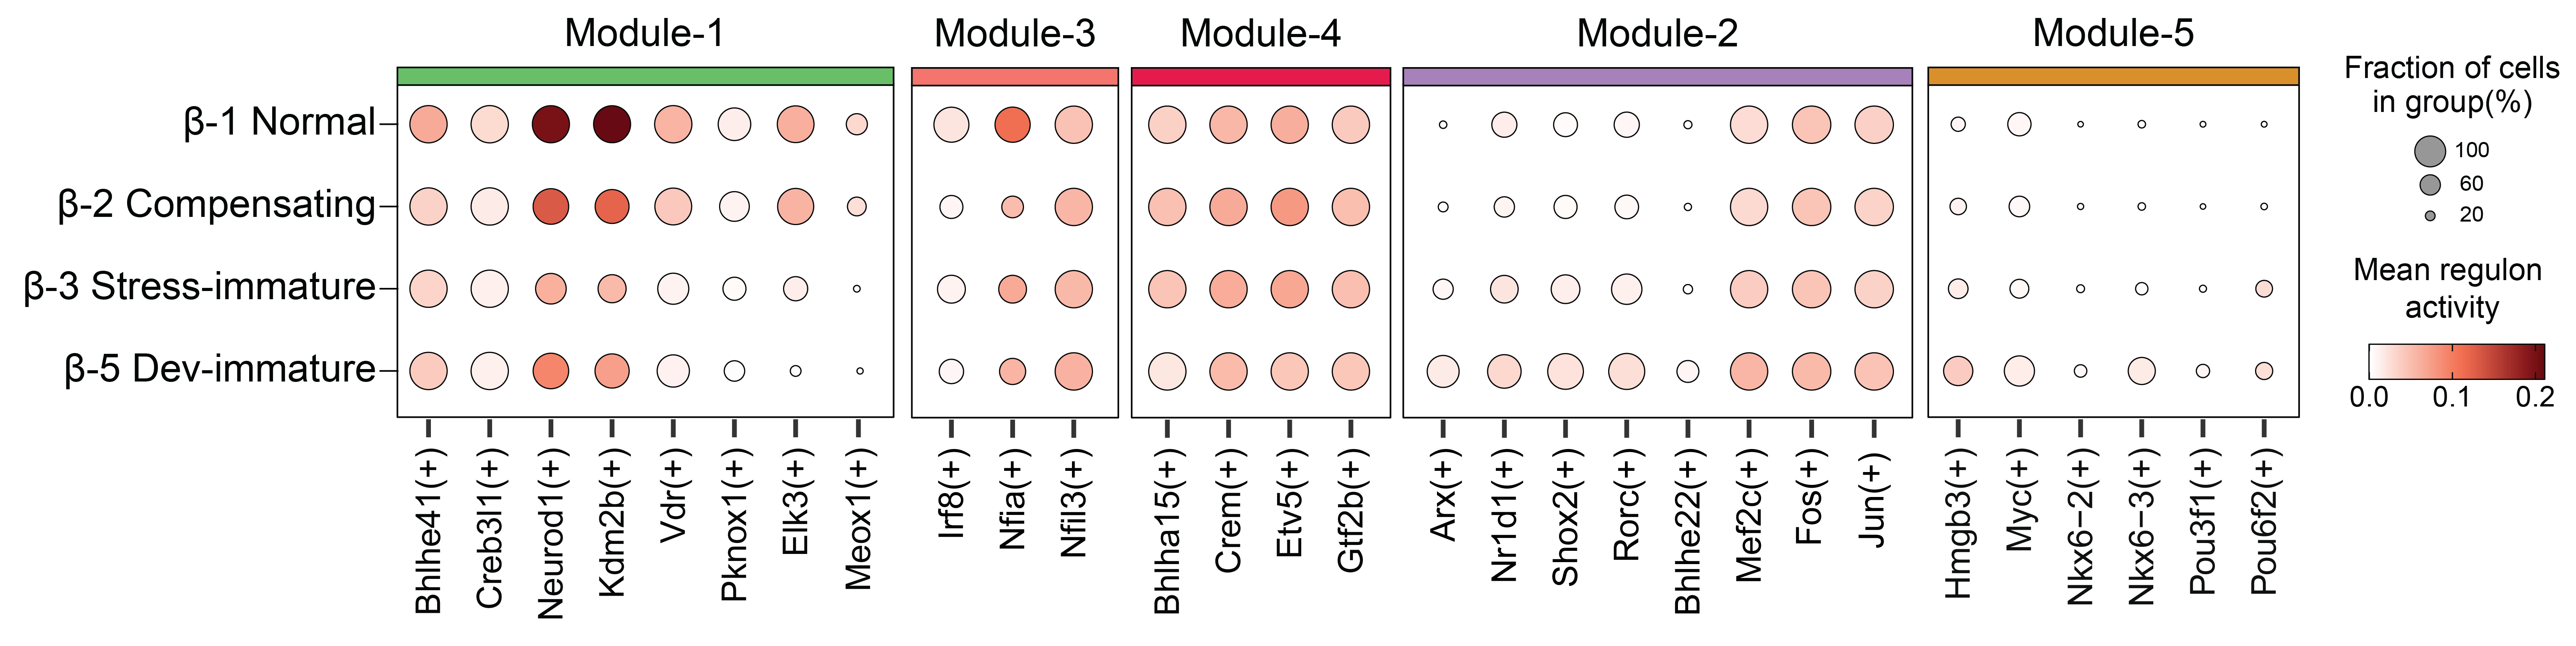
\includegraphics[width=\linewidth]{Chapter5/Fig/F3-12-v2-02.png}
% \caption[Activity of \glsentryshort{tf}-regulons complements $\beta$-cell subset annotations]{\textbf{Activity of \gls{tf}-regulons complements $\beta$-cell subset annotations.} Dot plot depicting the mean activity of the indicated regulons across $\beta$-1, $\beta$-2, $\beta$-3 and $\beta$-5 subsets. The regulons are grouped by modules identified based on hierarchical clustering of the regulons using \gls{csi} as a distance measure. The color of the dots indicate the mean activity and the size of the dots correspond to the fraction of cells in which the regulon is active.}
% \label{fig:chp3_scenic_betasubsets}
% \end{figure}

\par Among the regulons identified across the $\beta$-cells, Module 3 included members of the \gls{ifn} regulatory factors (Irf1, Irf7, Irf8 and Irf9) and the \glsentrylong{stat} (Stat1, Stat2 and Stat3) families \textbf{(\autoref{fig:chp3_scenic_betasubsets}; \autoref{fig:app_chp3_scenic_betasubsets}; \autoref{fig:app_chp3_scenic_studies})}. These families are crucial for regulating type-1 \gls{ifn} induction and its downstream effects \textbf{\cite{mogensen_irf_2019}}. The activation of these pathways within the islets is particularly relevant, considering the well-established role of chronic inflammation in the etiology of \gls{t2d} \textbf{\cite{boni-schnetzler_islet_2019}}. The regulons clustered within Module 4 might suggest an axis of $\beta$-cell heterogeneity that might not be fully captured at the transcriptomic level \textbf{(\autoref{fig:chp3_scenic_betasubsets}; \autoref{fig:app_chp3_scenic_betasubsets}; \autoref{fig:app_chp3_scenic_studies})}.\\

\par Conversely, the regulons within Module 5 demonstrated minimal coordinated activity among themselves as evidenced by the \gls{csi} metric \textbf{(\autoref{fig:chp3_scenic_betaonly} A)}. Overall, these regulons exhibited low individual regulon activity across the $\beta$-cell subsets \textbf{(\autoref{fig:app_chp3_scenic_betasubsets})} as well as across the experimental groups \textbf{(\autoref{fig:app_chp3_scenic_studies})}. Nevertheless, a few of the regulons in this module depicted higher activity in the $\beta$-3 stress-immature or the $\beta$-5 dev-immature subsets compared to $\beta$-1 or $\beta$-2 subsets. Examples of these regulons include Myc, Hmgb3, Nkx6-3 and Pou6f2 \textbf{(\autoref{fig:chp3_scenic_betasubsets}; \autoref{fig:app_chp3_scenic_betasubsets})}. In particular, c-Myc, a signal-dependent \gls{tf} \textbf{\cite{wortham_transcriptional_2021}}, plays a central role in regulating cell proliferation \textbf{\cite{dang_c-myc_1999}}. In $\beta$-cells, c-Myc serves as an inverse dual regulator of $\beta$-cell proliferation and maturity \textbf{\cite{puri_replication_2018}} and is required for metabolic stress–mediated $\beta$-cell expansion in young mice \textbf{\cite{rosselot_myc_2019}}. HMGB3, an evolutionarily conserved chromosome binding protein, has been demonstrated to regulate growth, migration, and apoptosis in gastric cancer cells \textbf{\cite{guo_knockdown_2016}}. Furthermore, HMGB3 is primarily active during embryogeneis, is diminished or silent in adult tissues 
 and is 99\% homologous to the mouse gene \textbf{\cite{guo_knockdown_2016,nemeth_hmgb3_2003}}. The higher regulon activity of Hmgb3 in the $\beta$-5 dev-immature subset aligns with previous findings, suggesting an important role for this regulon in $\beta$-cell maturation. Although the role of Hmgb3 in mouse $\beta$-cells is not well-defined, another family member, HMGB1, acts as a danger signal to alert innate immune responses in autoimmune disorders such as \gls{t1d} \textbf{\cite{zhang_hmgb1_2010}}. Additionally, HMGB1, in combination with \glsentryshort{il}-1, promotes islet inflammation and $\beta$-cell death \textbf{\cite{steer_interleukin-1_2006}} and plays a pivotal role in the pathogenesis of diabeteic complications \textbf{\cite{biscetti_high_2019}}. Given these findings, it is plausible that Hmgb3 might have similar roles in $\beta$-cell dysfunction and islet inflammation in \gls{t2d}.\\


%The up-regulation of these regulons could thus be indicative of an inflammatory state within the $\beta$-cells, potentially contributing to the dysfunction observed in \gls{t2d}.\\ % In particular, \textit{Stat1} is a master regulator of $\beta$-cell apoptosis and islet inflammation in \gls{t1d} \textbf{\cite{https://www.ncbi.nlm.nih.gov/pmc/articles/PMC3020778/}}. A type-1 \gls{ifn} response in islet macrophages was observed in response to metabolic stresses such as diet-induced obesity and aging in \textbf{\autoref{chp:diet_aging}}.  \textit{Kdm2b}, a lysine-specific demethylase, is a critical regulator of definitive hematopoiesis, mediates a gene repressive program that controls hippocampal morphogenesis, represses transcription of ribosomal RNA genes in human cell lines and inhibits the ability of \textit{Cdkn1a}/\textit{p21} to promote senescence in fibroblasts. %The largest module, \textit{Module 1}, contained TFs associated with $\beta$-cell function (\textit{Mafa, Nkx6-1}) and development (\textit{Neurod1, Pdx1}) \textbf{(Fig. \ref{fig:3-10})}. The mean regulon activity of \textit{Mafa} and \textit{Pdx1} was comparable across all subsets \textbf{(Fig. \ref{fig:3-12})}. The activity of \textit{Tcf7l2}, a master regulator of insulin production and processing, and its downstream target \textit{Isl1} were also similar across all subsets. Interestingly, the mean activity of \textit{Neurod1} regulon was (quantitatively) higher for $\beta$-1 Normal subset and was down-regulated in $\beta$-2 and $\beta$-3 subsets. Another interesting TF-regulon with similar activity and expression pattern is \textit{Kdm2b}. \hl{<Stuff about \textit{Kdm2b}>}. Module 1 also included \textit{Atf5}, which has been shown to be an important regulator of ER stress and apoptosis in mouse $\beta$-cells \textbf{\cite{ma_atf5_2023}}, and \textit{Hmgb1}, a chromatin protein that can induce autophagy by activating various pathways and has been shown to play an important role in insulin resistance and diabetes \textbf{\cite{yang_relationship_2023}} \textbf{(Fig. \ref{fig:3-12})}. \hl{<Stuff about \textit{Vdr}>}\\ %\textit{Module 2} was characterized by the presence of \textit{Fos} and \textit{Jun} regulons, which are components of the activator protein-1 (AP-1) TF complex, and are involved in stress response and have been implicated in the regulation of $\beta$-cell function, particularly under conditions of metabolic stress or diabetes. \textit{Jund}, a member of the \textit{Jun} family, in particular,  has been found to be up-regulated  in response to high concentrations of glucose and free fatty acids, and its depletion can block the increase in oxidative stress and apoptosis in $\beta$-cells during glucolipotoxicity \textbf{\cite{good_jund_2019}}. Strikingly, this module also contained the TF \textit{Arx}, which specifies the formation of pancreatic islet α-cell during development. The \textit{Arx} regulon was active in both, the $\beta$-3 Stress-immature and the $\beta$-5 Dev.-immature subsets. The higher activity of \textit{Arx} in $\beta$-3 compared to $\beta$-1 or $\beta$-2 subsets likely suggests the activation of a dedifferentiation like-program in response to increased workload in hyperglycemic and insulin-resistant models. The forced over-expression of \textit{Arx} within pancreata showed massive reductions in beta and delta cell numbers and increased alpha and PP cell numbers \textbf{\cite{van_der_meulen_role_2015}}. This (trans/de)-differentiation could be mitigated by the activity of \textit{Klf6} regulon, a downstream effector of \textit{Sox9} \textbf{\cite{puri_sox9_2024}} and an immediate early response gene \textbf{\cite{xin_single-cell_2016}}, in $\beta$-2 subset, as \textit{Klf6} has been shown to protect $\beta$-cells against insulin-resistance induced dedifferentiation. \textit{Klf6} knockout mice displayed stronger $\beta$-cell dysfunctions against insulin resistance (WD-feeding) with severe hyperglycemia (S961 treatment) \textbf{\cite{dumayne_klf6_2020}}. \hl{<Stuff about \textit{Taf7,Rorc}>}\\

%\textit{Module-3} contained the TFs \textit{Cebpb} and \textit{Cebpd}, which have anti-apoptotic and anti-inflammatory roles in pancreatic $\beta$-cells \textbf{\cite{https://www.ncbi.nlm.nih.gov/pmc/articles/PMC3275575/}}. This module was also comprised of members of the IFN regulatory factor (\textit{Irf1, Irf7, Irf8} and \textit{Irf9}) and the signal transducer and activator of transcription (\textit{Stat1,Stat2} and \textit{Stat3}) families, which have essential roles in regulating Type-1 IFN induction and downstream actions, respectively \textbf{\cite{https://www.ncbi.nlm.nih.gov/pmc/articles/PMC6331453/}}. In particular, \textit{Stat1} is a master regulator of $\beta$-cell apoptosis and islet inflammation \textbf{\cite{https://www.ncbi.nlm.nih.gov/pmc/articles/PMC3020778/}}. 

% The other two modules (Module 4 and Module 5) were comprised mostly of regulons that were either invariant across all non-proliferating $\beta$-cell subsets (Module 4) or did not depict any regulon activity in these subsets (Module 5) \textbf{(\autoref{fig:app_chp3_scenic_betasubsets}; \autoref{fig:app_chp3_scenic_studies})}. 



% \hl{\textit{Module 4} contained regulons such as \textit{Bach2, Bhlha15, Crem, E2f1, Etv5, Gtf2b, Hoxb2, Mybl1, Nr1h3} which seemed to be uniformly active across all $\beta$-subsets, whereas most of the regulons in \textit{Module 5} had no activity in any of the $\beta$-subsets. Of note, \textit{Hmgb3} regulon had higher activity in the $\beta$-5 Dev.-Immature subset compared to the rest and the \textit{Pou6f2} regulon had a similar profile in $\beta$-3 Stress-Immature and $\beta$-5 Dev.-Immature subsets.}\\

%\clearpage
% \begin{figure}[H]
% \centering
% \includegraphics[width=\linewidth]{Chapter5/Fig/F3-12-02.png}
% \caption[Mean regulon activity of all regulons in Module-2 of $\beta$-cell GRN]{\textbf{Mean regulon activity of all regulons in Module-2 of $\beta$-cell GRN}\\}
% \label{fig:3-12-2}
% \end{figure}



\par To gain a better understanding about the expression dynamics of \glspl{tf} regulons identified in this analysis, we examined the expression of several candidate \gls{tf} along the Maturity (\gls{pc}1)-Workload (\gls{pc}2) axis \textbf{(\autoref{fig:chp3_TFgenes})}. Consistent with previous observations, \glspl{tf} such as Mafa, Vdr, Atf5 and the histone demethylase Kdm2b were down-regulated with the loss of $\beta$-cell maturity in the $\beta$-3 subset and in the functionally immature $\beta$-5 subset \textbf{(\autoref{fig:chp3_TFgenes} A)}. Conversely, the expression of \glspl{tf} such as Egr1, Hmgb1, Mafb, Mlxipl and components of the AP-1 complex (Fos, Jun) correlated with the stress- and developmentally-immature $\beta$-cell subsets \textbf{(\autoref{fig:chp3_TFgenes} A)}. Along the workload axis, distinguishing the $\beta$-1 normal subset from the $\beta$-2 compensating and $\beta$-3 stress-immature subsets, the expression dynamics of these \glspl{tf} appeared less consistent, potentially due to high intercellular variability \textbf{(\autoref{fig:chp3_TFgenes} B)}. However, akin to patterns along \gls{pc}1, there was an overall down-regulation in expression of such as Mafa, Vdr, Kdm2b and Atf5 within the $\beta$-2 and $\beta$-3 subsets. Particularly interesting was the expression of nuclear factor IL-3 (\textit{Nfil3}), also known as E4 promoter-binding protein 4 (E4BP4), which showed increased expression along the workload axis \textbf{(\autoref{fig:chp3_TFgenes} B)}. A recent study depicted that under conditions of \gls{er} stress, the expression of E4BP4 is increased which dysregulates clock output gene DBP, thereby impairing circadian oscillation and disrupting $\beta$-cell function \textbf{\cite{ohta_clock_2017}}. Furthermore, the role of Nfil3 in insulin target tissues is becoming increasingly evident and suggests a putative role in diabetes \textbf{\cite{keniry_new_nodate}}.\\

\begin{figure}[t]
    \centering
    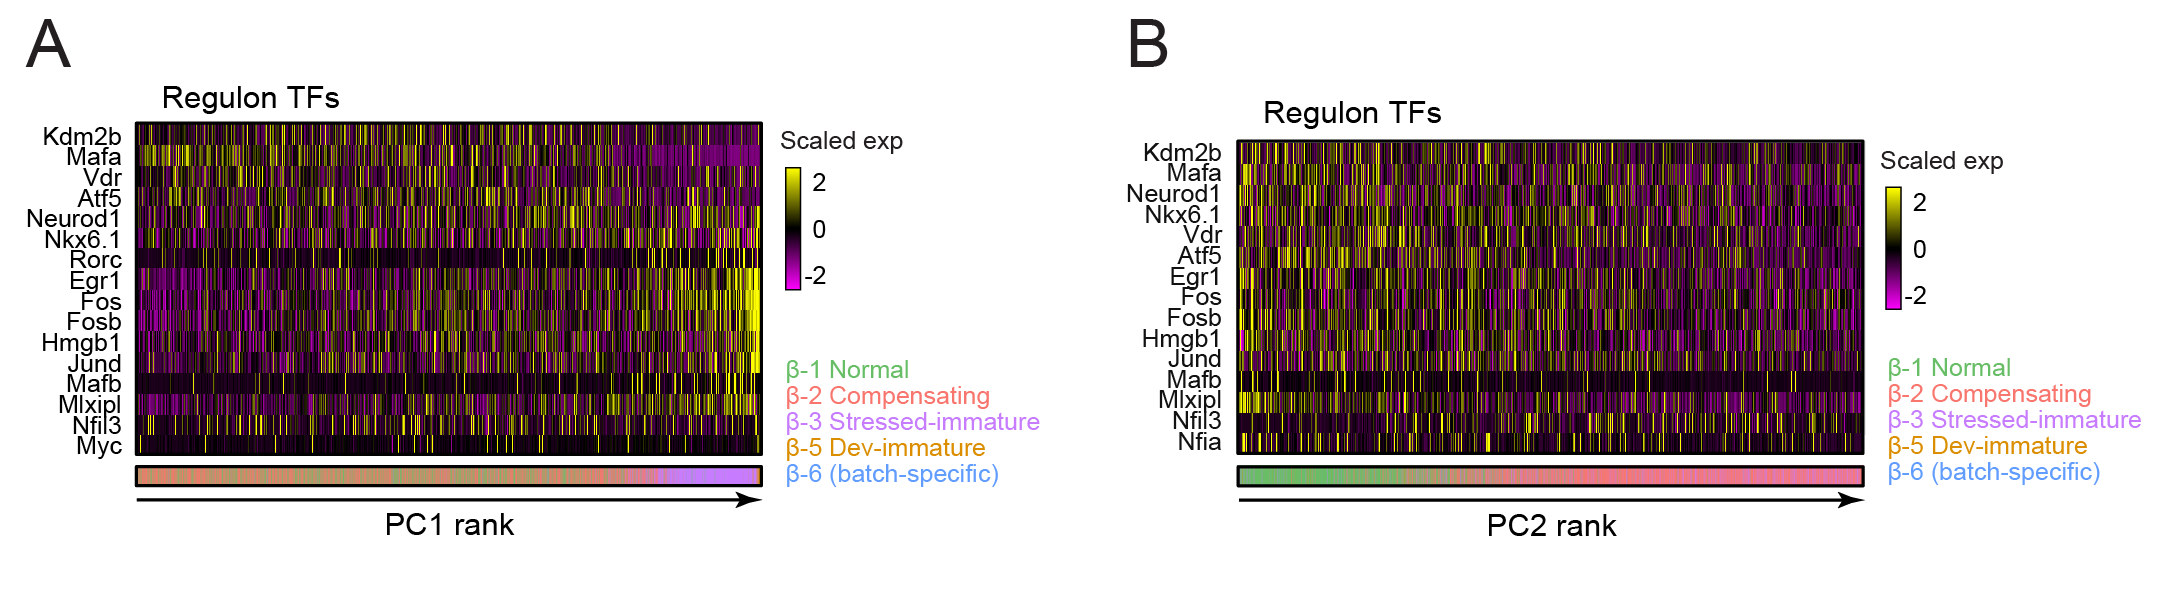
\includegraphics[width=\linewidth]{Chapter5/Fig/F3-19-01.png}
    \caption[Expression of regulon\glsentryshort{tf}s along the Maturity-Workload axes]{\textbf{Expression of regulon \glspl{tf} along the Maturity-Workload axes.} \textbf{(A) - (B)} Heatmap depicting the scaled expression of the indicated regulon \glspl{tf} (rows) across all non-proliferating $\beta$-cells ordered according to their ranks along \gls{pc}1 \textbf{(A)} or \gls{pc}2 \textbf{(B)}. The color bar below the heatmaps indicate the subset annotations. }
    \label{fig:chp3_TFgenes}
\end{figure}

\par In conclusion, we identified \glspl{grn} for \glspl{tf} known to impact $\beta$-cell identity and function as well as novel candidate \glspl{tf}. These \glspl{tf} and their target genes work in unison to effect the transcriptional heterogeneity of $\beta$-cell subsets. The underlying \glspl{grn} also play a crucial role in evoking the cellular response to environmental cues and maintaining $\beta$-cell identity and function under varying workload conditions.

%\clearpage

% Interestingly, while the expression of key \glspl{tf} like \textit{Neurod1} and \textit{Nkx6-1} in the $\beta$-5 Dev-immature subset is expected, they were also up-regulated with the loss of maturity in response to insulin resistance and hyperglycemia
%\clearpage

\begin{comment}

\section[Transcriptional similarity of mouse models to human \glsentryshort{t2d}]{Transcriptional similarity of mouse models to human \gls{t2d}}
\label{sec:chp3_T2Dgenes}

Rodent models are crucial for studying T2D, providing insights into disease pathogenesis, progression, and potential therapies due to their physiological similarities to humans. The different models vary in how closely they mimic the natural progression of human \gls{t2d} and have specific advantages and limitations \textbf{\cite{kleinert_animal_2018, singh_animal_2024}}. Given the broad range of $\beta$-cell workload models included in this study, we wanted to further asses the extent of similarity of transcriptional profiles of these models to human \gls{t2d}. Extending the assessment made by the \gls{mia} \textbf{\cite{hrovatin_delineating_2023}}, we utilized gene sets enriched in human \gls{t2d} identified in their analysis and scored for these gene sets across all non-proliferating $\beta$-cells in our integrated data \textbf{(}see \hyperref[subsubsec:met_chp3_scoring]{\textbf{Methods}}\textbf{)}. These included gene sets related to pancreas development, hormone metabolism, ribosome biogenesis, protein or peptide breakdown by proteasome and transport vesicle of the constitutive secretory pathways. Furthermore, we also assessed the level of up-regulation or down-regulation of several of the characteristic markers associated with these gene sets in order to obtain a gene-level understanding about the dynamics of $\beta$-cell workload in response to hyperglycemia and insulin resistance \textbf{(}see \hyperref[subsubsec:met_chp3_foldchanges]{\textbf{Methods}}\textbf{)}.

%The scores of these gene-sets across all non-proliferating $\beta$-cells were computed (see \hyperref[sec:chp4_methods2]{\textit{Methods}}). %For each of these gene-sets, we first identified the orthologous genes in our mouse dataset and then performed gene-set scoring on a single-cell level.\\Rodent models play a crucial role in the study of \gls{t2d}, offering insights into disease pathogenesis, progression and potential therapeutic interventions. These models are invaluable due to their physiological similarities to humans, including the snapshots of the pathogenesis and progression of \gls{t2d}. 

\subsubsection{Endocrine pancreas development}
\label{subsubsec:endopanc}
The gene set `endocrine pancreas development' was down-regulated in all samples compared to their respective controls \textbf{(\autoref{fig:chp3_gs_endo} A)} in all studies. This was also observed in the \gls{mia} which included a similar genetic obesity model (\textit{db/db} animals with established hyperglycemia) and the partial $\beta$-cell ablation model also included in our analysis. However, since this gene set was enriched among human \gls{t2d} up-regulated genes, the unexpected direction of the gene set change in the mouse \gls{t2d} models could be attributed to the diversity of the genes in this gene set. This included genes related to $\beta$-cell maturation as well as $\beta$-cell immaturity, which likely affected the scoring. We therefore examined specific genes from this gene set \textbf{(\autoref{fig:chp3_gs_endo} B)} by analyzing their expression trend in response to a given environmental stressor. The expression of several characteristic $\beta$-cell identity and functional genes in this gene set were mildly down-regulated in all stress models except in case of feeding intervention and insulin receptor blockade with S961. Genes such as \textit{Gipr, Neurod1, Nkx2-2, Nkx6-1} were mildly up-regulated in the fed mice whereas S961 treatment induced the up-regulation of \textit{Foxa2, Insm1, Nkx2-2}  and \textit{Pdpk1}. This discrepancy could reflect species differences in \gls{t2d} pathogenesis.

\begin{figure}[t]
\centering
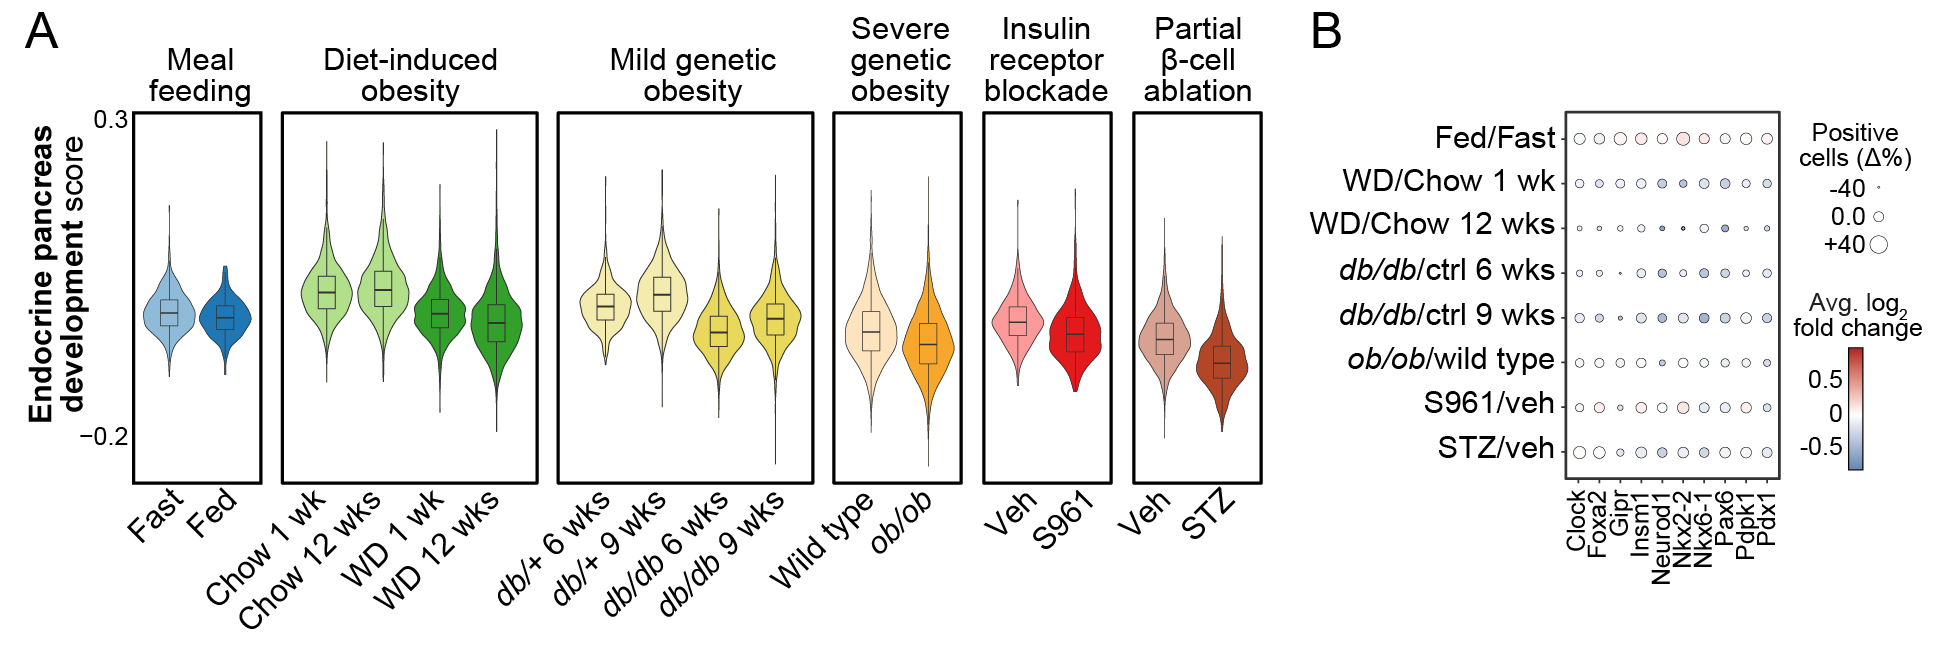
\includegraphics[width=\linewidth]{Chapter5/Fig/F3-13-01.png}
\caption[Activity of genes associated with endocrine pancreas development]{\textbf{Activity of genes associated with Endocrine pancreas development.} \textbf{(A)} Violin plots depicting the gene set score for Endocrine pancreas development associated genes shown for $\beta$-cell workload models and corresponding healthy controls from individual studies. On the overlay box plots, the middle horizontal line represents the median, the box represents the inter-quartile range and the whiskers represent the minimum and maximum values. The number of cells are indicated in \textbf{\autoref{tab:app_chp3_cellnumbers}}. \textbf{(B)} Differential expression of the indicated genes from the Endocrine pancreas development gene set $\beta$-cell workload models compared to their respective controls. The color and size of the dots represent the average $\log\textsubscript{2}$ fold change of expression and the difference in percentage of cells between the samples and their respective controls.}
\label{fig:chp3_gs_endo}
\end{figure}%\clearpage

\subsubsection{Hormone metabolism}
Similar to the observations in \gls{mia}, genes related to hormone metabolic processes were strongly up-regulated in most models $\beta$-cell workload, with the exception of meal feeding model \textbf{(\autoref{fig:chp3_gs_hm} A)}. The lack of observed up-regulation of genes related to hormone metabolism could be, in part, explained by the acute timeline between feeding and fasting groups, compared to the chronic \gls{wd} feeding or the hyperglycemic environ-



\begin{figure}[H]
\centering
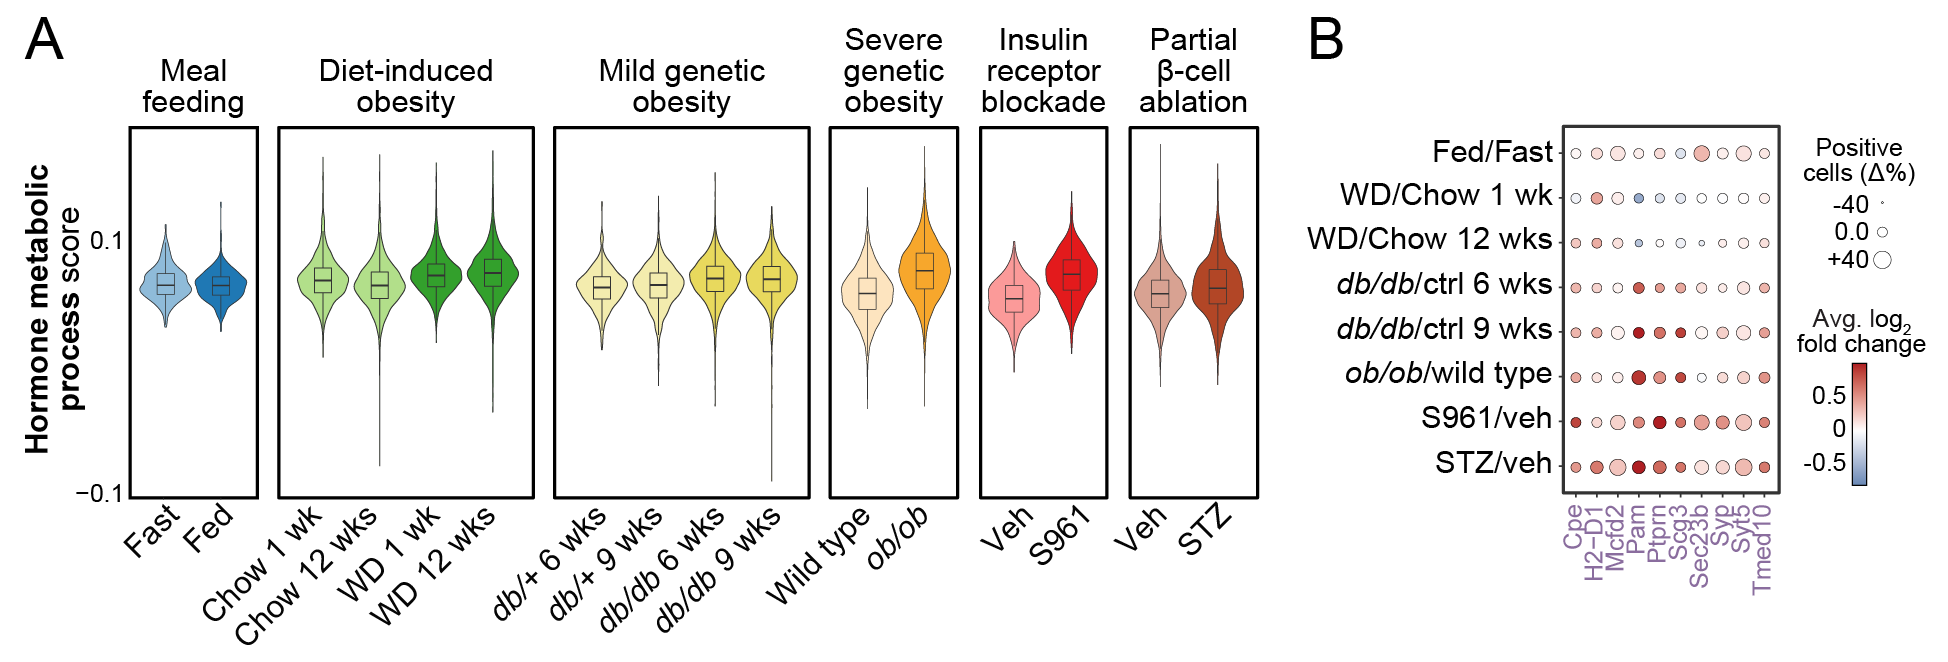
\includegraphics[width=\linewidth]{Chapter5/Fig/F3-13-02.png}
\caption[Activity of genes associated with hormone metabolic processes]{\textbf{Activity of genes associated with Hormone metabolic process.} \textbf{(A)} Violin plots depicting the gene set score for Hormone metabolic process associated genes shown for $\beta$-cell workload models and corresponding healthy controls from individual studies. On the overlay box plots, the middle horizontal line represents the median, the box represents the inter-quartile range and the whiskers represent the minimum and maximum values. The number of cells are indicated in \textbf{\autoref{tab:app_chp3_cellnumbers}}. \textbf{(B)} Differential expression of the indicated genes from the Hormone metabolic process gene set across $\beta$-cell workload models compared to their respective controls. The color and size of the dots represent the average $\log\textsubscript{2}$ fold change of expression and the difference in percentage of cells between the samples and their respective controls.}
\label{fig:chp3_gs_hm}
\end{figure}

% \boldlink{https://doi.org/10.1016/0092-8674(94)90296-8} \boldlink{https://doi.org/10.2337/diabetes.50.3.534} \boldlink{https://doi.org/10.1016/j.molmet.2022.101595} \boldlink{https://doi.org/10.1016/j.cmet.2016.08.020}

-ments induced by genetic obesity or chemical treatments. The strongly up-regulated genes included \textit{Ttr, Scg5, Cpe} and \textit{Atp1a1}. \textit{Ttr} is a transport protein and is known to constitute a functional component in normal pancreatic $\beta$-cell stimulus-secretion coupling and also preserves $\beta$-cell integrity \textbf{\cite{refai_transthyretin_2005}}. \textit{Scg5} is a molecular chaperone for \textit{Pcsk2}, a gene that encodes enzyme that cleaves pro-hormones, including insulin, IAPP and glucagon \textbf{\cite{tritschler_transcriptional_2022,segerstolpe_single-cell_2016}}. A \gls{scr} study found that SCG5 expression was up-regulated in a stressed human $\beta$-cell state \textbf{\cite{tritschler_transcriptional_2022}} and another \gls{scr} study identified that SCG5 expression was negatively correlated with increasing BMI, thereby implicating a $\beta$-cell dysfunction in hormone processing \textbf{\cite{segerstolpe_single-cell_2016}}. Defective maturation of proinsulin is implicated in both \gls{t1d} and \gls{t2d} \textbf{\cite{tritschler_transcriptional_2022}}. The apparent coordinated up-regulated expression of \textit{Ttr} and \textit{Scg5} could be indicative of increased insulin processing and secretion by $\beta$-cells in response to increased workloads and hyperglycemic conditions. Of note, the S961 treatment induced a stronger up-regulation of \textit{Cpe} and \textit{Atp1a1} compared to other studies. \textit{Cpe} is involved in proinsulin processing \textbf{\cite{davidson_insulin-secretory-granule_1987}}, and $\beta$-cell specific deletion of \textit{Cpe} led to elevated proinsulin output, which likely reshapes $\beta$-cell glucose metabolism and increases its susceptibility to secretory stress–induced dysfunction and diabetes \textbf{\cite{chen_deletion_2023}}. \textit{Atp1a1} encodes the principal subunit of Na\textsuperscript{+}/K\textsuperscript{+} \glslink{atp}{ATP}-ase which is a key regulator of the the insulin secretion pathway and is required for membrane depolarization preceding the insulin granule release \textbf{\cite{saini_functional_2016}}. Overall, enhanced insulin processing and secretion is observed in response to increased workloads and hyperglycemic conditions across all but one studies compiled in this meta-analysis. 

% mutations in this gene lead to obesity and hyperglycemia in mice and humans. Furthermore, reduced expression of \textit{Cpe} is associated with multiple experimental models of diabetes. A study exploring the role of \textit{Cpe} in $\beta$-cells demonstrated that the $\beta$-cell specific deletion of \textit{Cpe} alone did not contribute to obesity or cause marked dysglycemia. Interestingly, \textit{Cpe} deletion in mice administered with multiple low doses of \gls{stz} accelerated the development of hyperglycemia. % The strong up-regulation of several characteristic genes in the young \textit{db/db} animals was complementary to the up-regulation observed in older \textit{db/db} animals employed in the \gls{mia}.   %, \textit{}  %phogrin - 



%- (), secretogranin 3 (\textit{Scg3}) 


\subsubsection{Ribosome Biogenesis}
%Ribosomes are cellular factories that make proteins. 
Following a similar profile to `hormone Metabolism', the genes associated with the `ribosome biogenesis' gene set were up-regulated in both models of genetic obesity (\textit{db/db} and \textit{ob/ob}) and following S961- and \gls{stz}-treatment \textbf{(\autoref{fig:chp3_gs_rb} A)}. The feeding intervention and \gls{wd}-induced obesity did not result in a higher overall expression of this gene set \textbf{(\autoref{fig:chp3_gs_rb} A)}, and several genes were down-regulated in response to these two mild hyperglycemic models \textbf{(\autoref{fig:chp3_gs_rb} B)}. This echoes a similar observation of reduced expression of several ribosome biogenesis genes in a \gls{hfd} model. \textbf{\cite{hatanaka_chronic_2017}}. A significant increase in the expression of ribosome-related molecules has also been demonstrated in islets isolated from \textit{db/db} mice \textbf{\cite{asahara_increased_2009}}. The strong up-regulation of ribosomal markers in the \textit{ob/ob} mice and following S961 or \gls{stz} treatment could be attributed to the hyperglycemic environment leading to compensatory, increased insulin production \textbf{(\autoref{fig:chp3_gs_rb} B)}. The up-regulation of the ribosomal markers in the three hyperglycemic models was also consistent with the expression of ribosomal protein genes correlating with loss of $\beta$-cell maturity along the the Maturity (\gls{pc}1) axis \textbf{(\autoref{fig:chp3_pc1} B)}.

% and this effect is amplified in case of \gls{stz}-treatment, where the surviving population of $\beta$-cells following ablation are unable to prevent hyperglycemia 

\begin{figure}[H]
\centering
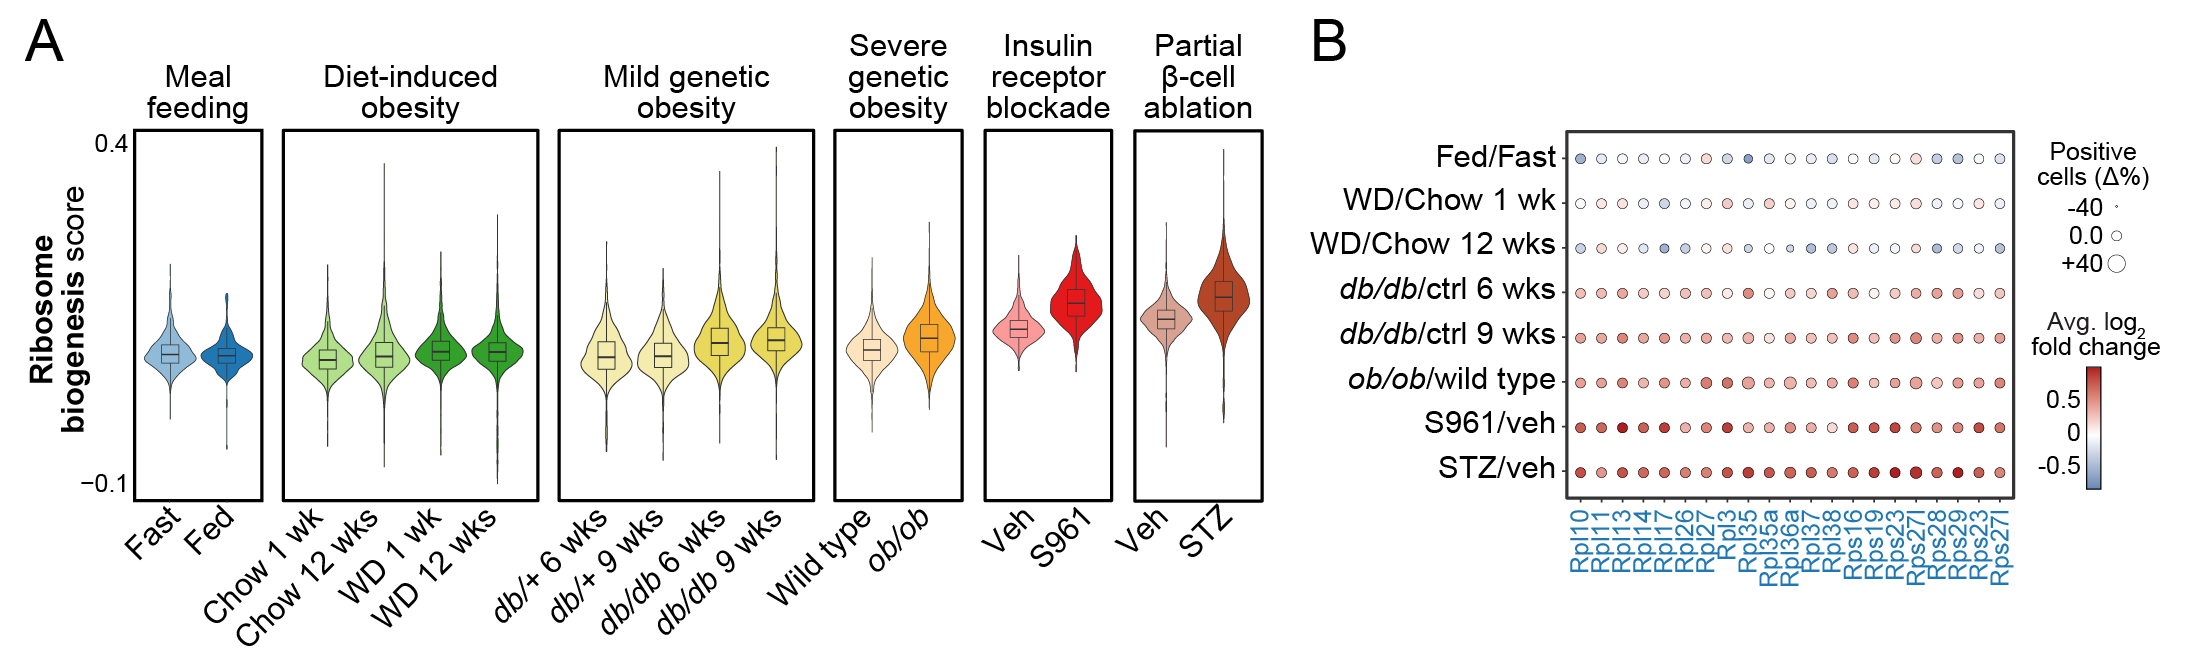
\includegraphics[width=\linewidth]{Chapter5/Fig/F3-13-03.png}
\caption[Activity of genes associated with ribosome biogenesis]{\textbf{Activity of genes associated with Ribosome biogenesis.} \textbf{(A)} Violin plots depicting the gene set score for Ribosome biogenesis associated genes shown for $\beta$-cell workload models and corresponding healthy controls from individual studies. On the overlay box plots, the middle horizontal line represents the median, the box represents the inter-quartile range and the whiskers represent the minimum and maximum values. The number of cells are indicated in \textbf{\autoref{tab:app_chp3_cellnumbers}}. \textbf{(B)} Differential expression of the indicated genes from the Ribosome biogenesis gene set across $\beta$-cell workload models compared to their respective controls. The color and size of the dots represent the average $\log\textsubscript{2}$ fold change of expression and the difference in percentage of cells between the samples and their respective controls.}
\label{fig:chp3_gs_rb}
\end{figure}


\subsubsection{Proteasomal catabolic process}
The gene set `proteasomal catabolic process' was up-regulated in all models of increasing $\beta$-cell workload \textbf{(\autoref{fig:chp3_gs_pcp} A)}. The genes comprising this gene set were canonical \gls{upr} and \gls{erad} markers. The \gls{upr} is a critical adaptive response to \gls{er} stress, restoring cell homeostasis and contributing to loss of $\beta$-cell mass in \gls{t2d} \textbf{\cite{oppenlander_vertical_2021,fonseca_endoplasmic_2011,bilekova_pharmacological_2021}}. However, unmitigated \gls{er} stress shifts the \gls{upr} to a terminal signaling  

\begin{figure}[H]
\centering
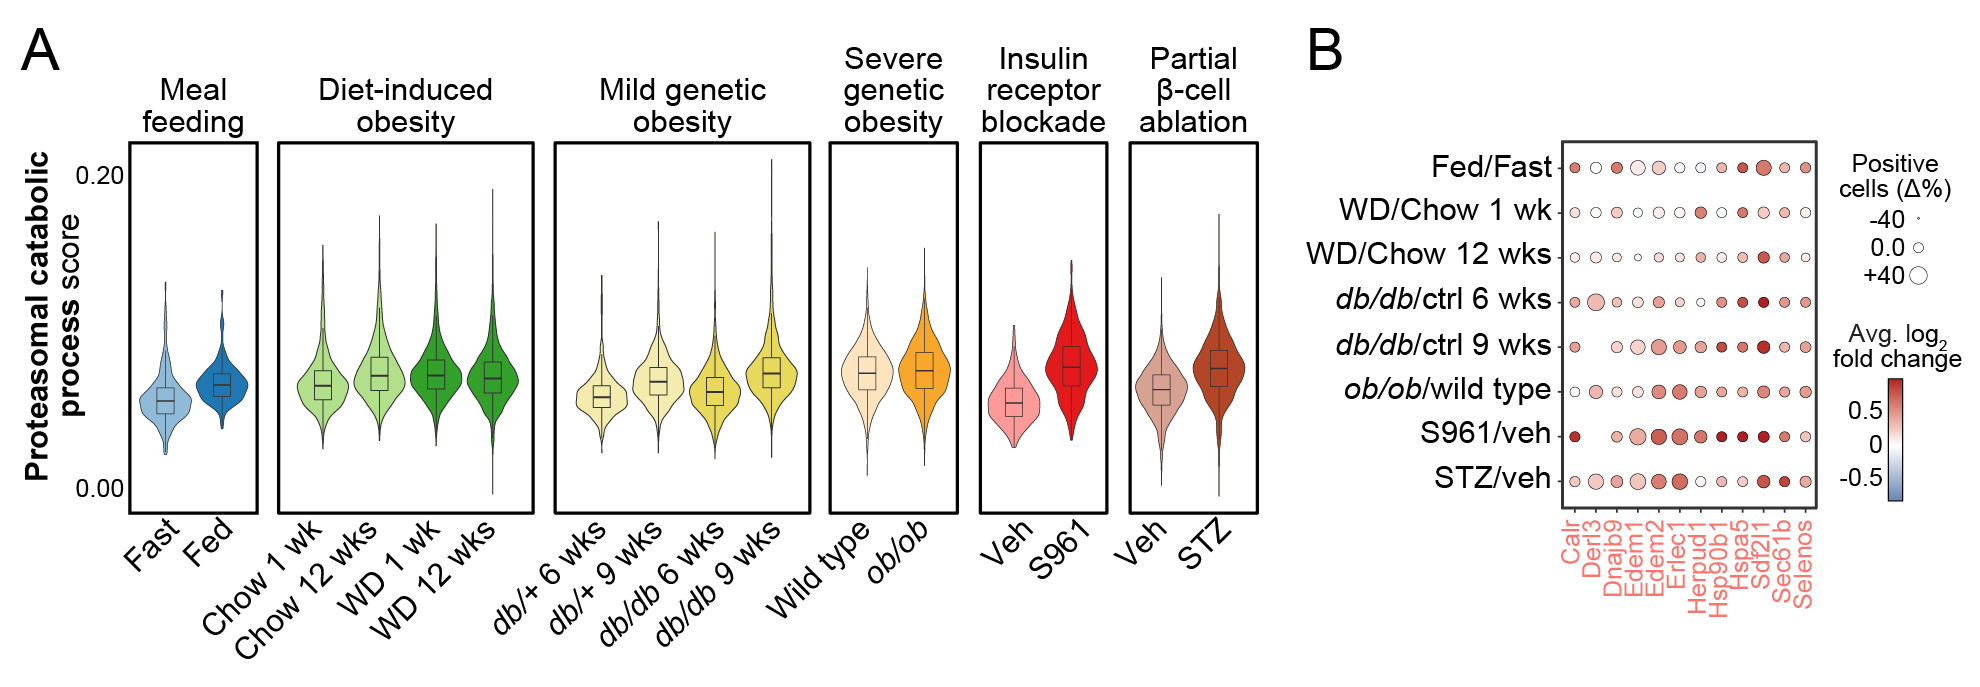
\includegraphics[width=\linewidth]{Chapter5/Fig/F3-13-04.png}
\caption[Activity of genes associated with proteasomal catabolic process]{\textbf{Activity of genes associated with Proteasomal catabolic process.} \textbf{(A)} Violin plots depicting the gene set score for Proteasomal catabolic process associated genes shown for $\beta$-cell workload models and corresponding healthy controls from individual studies. On the overlay box plots, the middle horizontal line represents the median, the box represents the inter-quartile range and the whiskers represent the minimum and maximum values. The number of cells are indicated in \textbf{\autoref{tab:app_chp3_cellnumbers}}. \textbf{(B)} Differential expression of the indicated genes from the Proteasomal catabolic process gene set across $\beta$-cell workload models compared to their respective controls. The color and size of the dots represent the average $\log\textsubscript{2}$ fold change of expression and the difference in percentage of cells between the samples and their respective controls.}
\label{fig:chp3_gs_pcp}
\end{figure}


cascade, culminating in $\beta$-cell apoptosis \textbf{\cite{ghosh_endoplasmic_2019}}. \gls{upr} genes such as \textit{Hspa5, Edem2, Derl3} and \textit{Herpud1} were found to be up-regulated on the \gls{mrna} level in response to various models of increasing $\beta$-cell workload \textbf{(\autoref{fig:chp3_gs_pcp} B)}. The \gls{erad} pathway serves to mitigate \gls{er} stress and has been attributed an indispensable role in the maintenance of $\beta$-cell identity and function \textbf{\cite{oppenlander_vertical_2021,hu_endoplasmic_2019,shrestha_sel1l-hrd1_2020}}. The expression of \gls{erad} genes such as \textit{Derl3, Dnajb9, Edem1/2, Herpud1, Hspa5, Hsp90b1, Sec61b, Selenos} were also up-regulated in all studies \textbf{(\autoref{fig:chp3_gs_pcp} B)}. Therefore, increases in $\beta$-cell workload enhances adaptive-response mechanisms to \gls{er} stress in $\beta$-cells in order to prevent $\beta$-cell failure. 

\subsubsection{Transport vesicle}
Diet models such as meal feeding and diet-induced obesity exhibited opposite patterns for the Transport vesicle gene set \textbf{(\autoref{fig:chp3_gs_tv} A)}. Feeding intervention resulted in the up-regulation of the gene set whereas \gls{wd} feeding for 1 or 12 weeks down-regulated the overall gene set \textbf{(\autoref{fig:chp3_gs_tv} B)}. This discrepancy could be explained by an acute increase in transport vesicle dynamics upon feeding compared to chronic effects of obesity induced by \gls{wd} feeding resulting in the down-regulation of these processes. Furthermore, it is plausible that the food composition of the \gls{wd} could be responsible for this unique effect to repress these genes, as all other models were fed a chow diet. Genetic predisposition to diabetes via the \textit{db/db} and \textit{ob/ob} models also exhibited an up-regulation of the vesicle gene set, although the magnitude in the \textit{ob/ob} model was lower \textbf{(\autoref{fig:chp3_gs_tv} A)}. The treatment-induced hyperglycemic models such as S961-treatment and \gls{stz}-treatment were strongly associated with changes in transport vesicle (\textit{Atp1a1, Stub1}) \textbf{(\autoref{fig:chp3_gs_tv} B)}.

\begin{figure}[H]
\centering
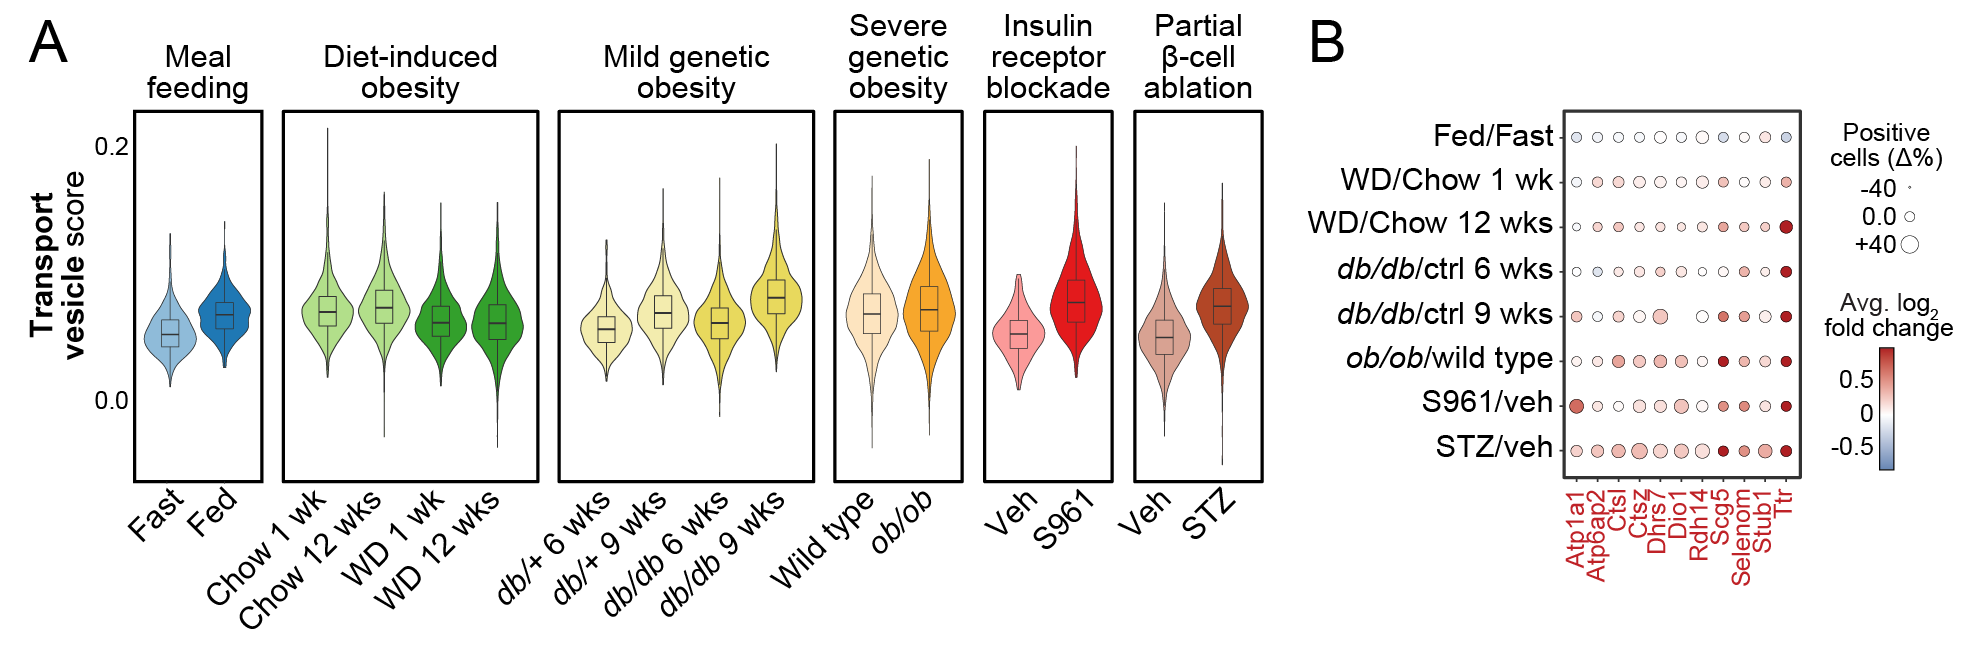
\includegraphics[width=\linewidth]{Chapter5/Fig/F3-13-05.png}
\caption[Activity of genes associated with transport vesicle]{\textbf{Activity of genes associated with Transport vesicle.} \textbf{(A)} Violin plots depicting the gene set score for Transport vesicle associated genes shown for $\beta$-cell workload models and corresponding healthy controls from individual studies. On the overlay box plots, the middle horizontal line represents the median, the box represents the inter-quartile range and the whiskers represent the minimum and maximum values. The number of cells are indicated in \textbf{\autoref{tab:app_chp3_cellnumbers}}. \textbf{(B)} Differential expression of the indicated genes from the Transport vesicle gene set across $\beta$-cell workload models compared to their respective controls. The color and size of the dots represent the average $\log\textsubscript{2}$ fold change of expression and the difference in percentage of cells between the models and their respective controls.}
\label{fig:chp3_gs_tv}
\end{figure}


Genes such as \textit{Pam, Ptprn, Scg3} were up-regulated in both 6-week-old and 9-week-old \textit{db/db} animals, with \textit{Ptprn, Scg3} depicting stronger up-regulation at the 9-week-old time-point \textbf{(\autoref{fig:chp3_gs_tv} B)}. \textit{Ptprn}, which is primarily localized on insulin secretory granules in $\beta$-cells, plays a crucial role in the overall regulation of glucose-stimulated insulin signalling in $\beta$-cells \textbf{\cite{torii_pseudophosphatase_2018}}. \textit{Scg3} plays a crucial role in regulating biogenesis of secretory granules that contain hormones in endocrine cells and assists in insulin processing, thus affecting glucose homeostasis \textbf{\cite{lin_serum_2019}}. These genes were also up-regulated in the hyperglycemic models of severe genetic obesity, insulin receptor blockade and the partial $\beta$-cell ablation. Hyperglycemia induced by chemical treatments (S961 and \gls{stz}) also resulted in stronger up-regulation of additional genes such as \textit{Cpe, Syp, Syt5} and \textit{Tmed10} \textbf{(\autoref{fig:chp3_gs_hm} B)}.\\


%This strong up-regulation could be a result of activation of responses to cellular stress as way for $\beta$-cells to maintain function by increasing the expression of genes.\\

\par In summary, $\beta$-cell compensatory responses to heightened demands of increased workload resulted in overall down-regulation of markers related to $\beta$-cell identity and function and up-regulated pathways related to hormone metabolism, ribosomal biogenesis, vesicle trafficking and \gls{er} stress. The coordinated up-regulation of processes related to hormone metabolism, ribosome biogenesis and vesicle transport could be an attempt by $\beta$-cells to enhance insulin production and secretion in response to increasing workloads and hyperglycemia. Overall, this analysis served as extension to the \gls{mia} by recapitulating the findings of similarity between human \gls{t2d} and mouse models of $\beta$-cell dysfunction in the context of mild and severe hyperglycemia.

%diet and feeding induced stress, severe genetic obesity and insulin receptor blockade by S961-treatment. % hormone metabolism and proteasomal catabolic processes and up-regulated cellular maesicle trafficking. chinery related to ribosomal biogenesis and vesicle trafficking. 

%\clearpage

\end{comment}

\section[$\beta$-cell subset shifts in response to unrestrained insulin secretion during obesity]{$\beta$-cell subset shifts in response to unrestrained insulin\\secretion during obesity}
\label{sec:chp3_validation}

%A major advantage of single-cell atlases is the ability to learn and transfer the findings from a reference study onto an external query dataset. This is particularly useful in cases of cell-type or state transfer between two or more studies as well as for comprehensive comparisons across several studies and/or conditions. Reciprocally, the atlases can benefit from transfer learning as it enhances the utility and applicability of these resources. The mapping of wide-variety of single-cell datasets exploring various aspects of development, health and disease onto references ultimately extends the scope of the atlases, thereby allowing for further refinement of cell-type annotation, improved data integration and robustness to data variability and facilitating discovery of novel biological insights.

\par The capacity to learn and apply the results from a reference study onto an external query dataset is a significant benefit of single-cell atlases \textbf{\cite{lotfollahi_mapping_2021,lotfollahi_biologically_2023,ye_mapping_2024}}. This is especially helpful for thorough comparisons across multiple studies and/or conditions, as well as for cell-type or state transfer between two or more studies. Reciprocally, atlases can benefit from transfer learning, as it enhances the utility and applicability of these resources. The mapping of a wide variety of single-cell datasets exploring various aspects of development, health, and disease onto references ultimately extends the scope of the atlases. This allows for further refinement of cell-type annotation, improved data integration and robustness to data variability, and facilitates the discovery of novel biological insights.\\

\par To demonstrate the usefulness of the integrated $\beta$-cell transcriptome atlas generated in this study, we mapped an external mouse dataset onto this reference. This additional study included an in-house generated dataset of islets from lean and obese, insulin resistant \textit{db/db} mice, with $\beta$-cell specific knockout of lysine-specific histone demethylase 1 (\textit{Lsd1}), which restrains the adaptive insulin secretion of $\beta$-cells in response to feeding \textbf{(\autoref{tab:app_chp3_study};} see \hyperref[subsubsec:met_chp3_data]{\textbf{Methods}}\textbf{)} \textbf{\cite{wortham_nutrient_2023}}. The dataset was generated using the 10x \gls{scr} workflow and the raw data was re-processed using the same workflow for sample processing and \gls{qc} in the integrated atlas. This ensured that technical batch effects did not influence the subsequent mapping steps. The dataset was projected onto the integrated $\beta$-cell subset in order to transfer the $\beta$-cell subset annotations from the reference to the query.

\subsubsection{\large Regulation of adaptive insulin secretion by the epigenome}

In a recent study, Wortham \textit{et al.} elucidated the nuanced regulation of $\beta$-cell functional adaptation by the epigenome, whereby nutrient availability modulates $\beta$-cell responses through histone hyperacetylation and transcription. Central to this regulation is the chromatin modifying enzyme lysine-specific histone demethylase 1 (\textit{Lsd1}) that acts as a dynamic regulator of histone acetylation in response to acute changes in nutrient state during feeding and fasting cycles. Interestingly, in an insulin-resistant model of $\beta$-cell adaptation (\textit{db/db}), the analysis also found overlap with genes up-regulated in acute $\beta$-cell response to feeding along with hyperacetylation at many of the feeding-induced sites. Thus, these findings support a model whereby $\beta$-cell adaptation of the insulin secretory response is regulated at the level of the epigenome, with influences from environmental nutrient signals and genetic variation \textbf{\cite{wortham_nutrient_2023,aamodt_peeling_2023}}.

%unveiled the islet epigenome as a pivotal regulatory layer in the $\beta$-cell functional adaptation to changes in insulin demand. Through integrated studies of β cell physiology, epigenomics, and transcriptomics \\Additionally, \textit{Lsd1}-bound active chromatin was also enriched for \gls{t2d}-associated risk variants, suggesting that \gls{t2d} risk variants can influence the activity of the \textit{Lsd1}-regulated network

\subsubsection{\large \textit{Lsd1} deletion worsens $\beta$-cell adaptation to obesity}


%To further understand why $\beta$-cells fail in \textit{Lsd1} knockout obese \textit{db/db} mice, 
To dissect the role of \textit{Lsd1} in $\beta$-cell compensatory mechanisms during insulin resistance, we crossed homozygous (\textit{db/db}) obese animals and their corresponding heterozygous (\textit{db/+}) lean mice with \textit{Lsd1\textsuperscript{fl/fl}} mice, in order to conditionally knockout \textit{Lsd1} in $\beta$-cells of adult mice using tamoxifen-inducible \textit{Pdx1-CreER} \textbf{(\autoref{fig:chp3_valid_study_design} A)}. We isolated islets from these animals prior to and after the onset of glucose intolerance and performed \gls{scr} \textbf{(\autoref{fig:chp3_valid_study_design} B)}. \textit{Lsd1} deletion in the lean mice caused severe hypoglycemia, whereas, surprisingly, \textit{Lsd1} knock out in the obese \textit{db/db} mice resulted in persistent hyperglycemia, thereby worsening the development of diabetes \textbf{(\autoref{fig:chp3_valid_study_metab} A)}. This was associated with reduced circulating insulin levels, suggesting an inherent functional $\beta$-cell defect underlying disease acceleration following \textit{Lsd1} deletion \textbf{(\autoref{fig:chp3_valid_study_metab} B)}. Contrary to observations \textit{in-vivo}, isolated islets from the \textit{db/db} animals with \textit{Lsd1} deletion hyper-secreted insulin in response to glucose. However, in response to secretagogues such as Exendin-4 (Ex-4), a functional analog of \gls{glp1}, and \gls{gip}, the normally robust response of \textit{db/db} islets was impaired following \textit{Lsd1} deletion in $\beta$-cells. This indicated that the failure to appropriately increase insulin secretion in response to incretin hormones --

\begin{figure}[t]
    \centering
    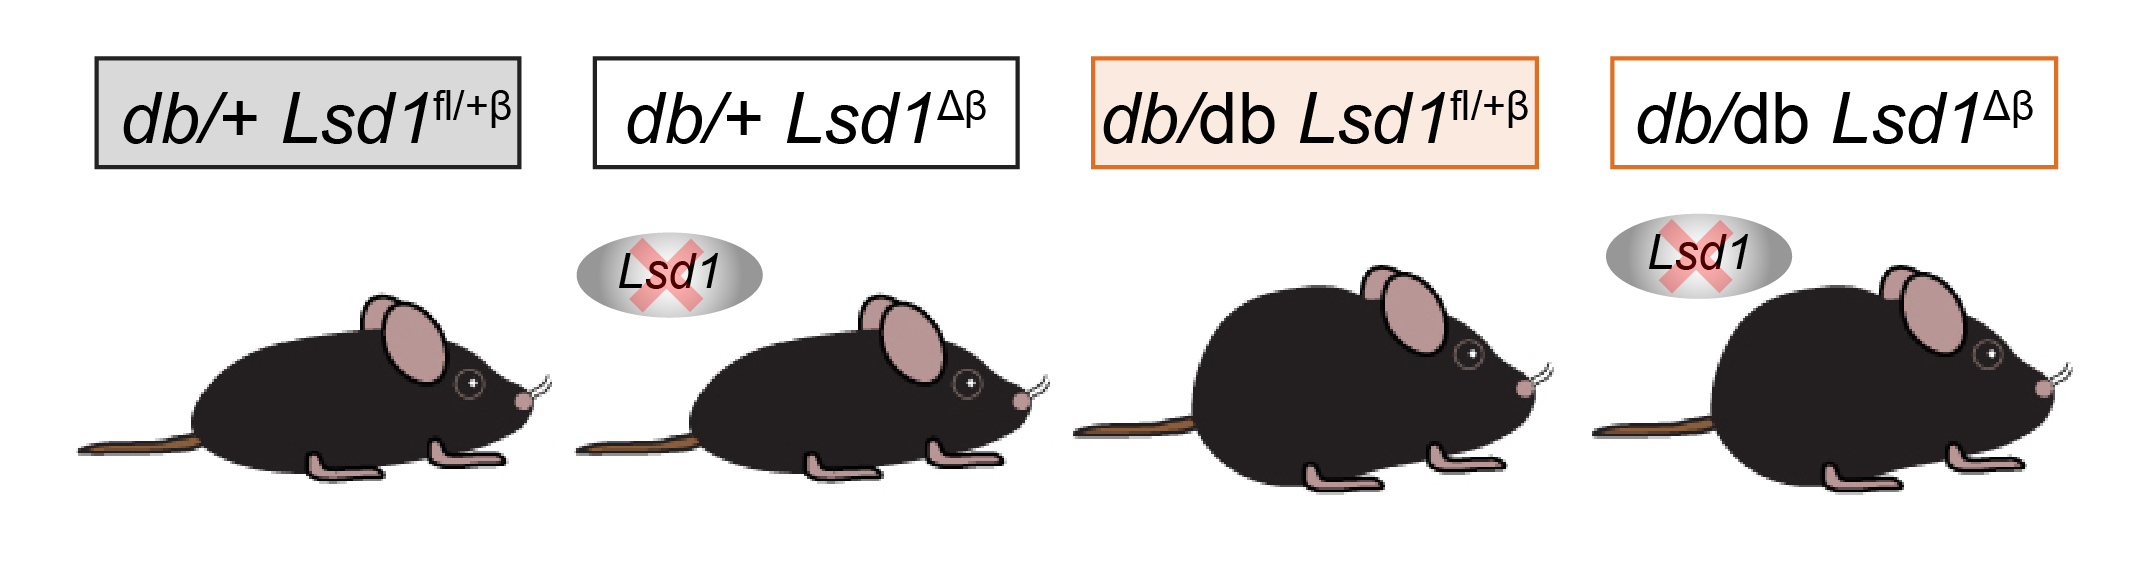
\includegraphics[width=\linewidth]{Chapter5/Fig/F3-17-02.png}
    \caption[Illustration of the experimental groups in the external study]{\textbf{Illustration of the experimental groups in the external study.} \textbf{(A)} Schematic of alleles and treatments used to inactivate \textit{Lsd1}. \textbf{(B)} Islets from lean (\textit{db/+}) and obese (\textit{db/db}) mice with or without intact \textit{Lsd1} in $\beta$-cells were isolated and dissociated single cells further processed with the 10x Genomics Chromium technology workflow. Abbreviations: TM, tamoxifen; q2d, every other day. \textit{This figure was originally generated by Dr. Matthew Wortham and has been adapted here with permission.}}
    \label{fig:chp3_valid_study_design}
\end{figure}

\begin{figure}[H]
    \centering
    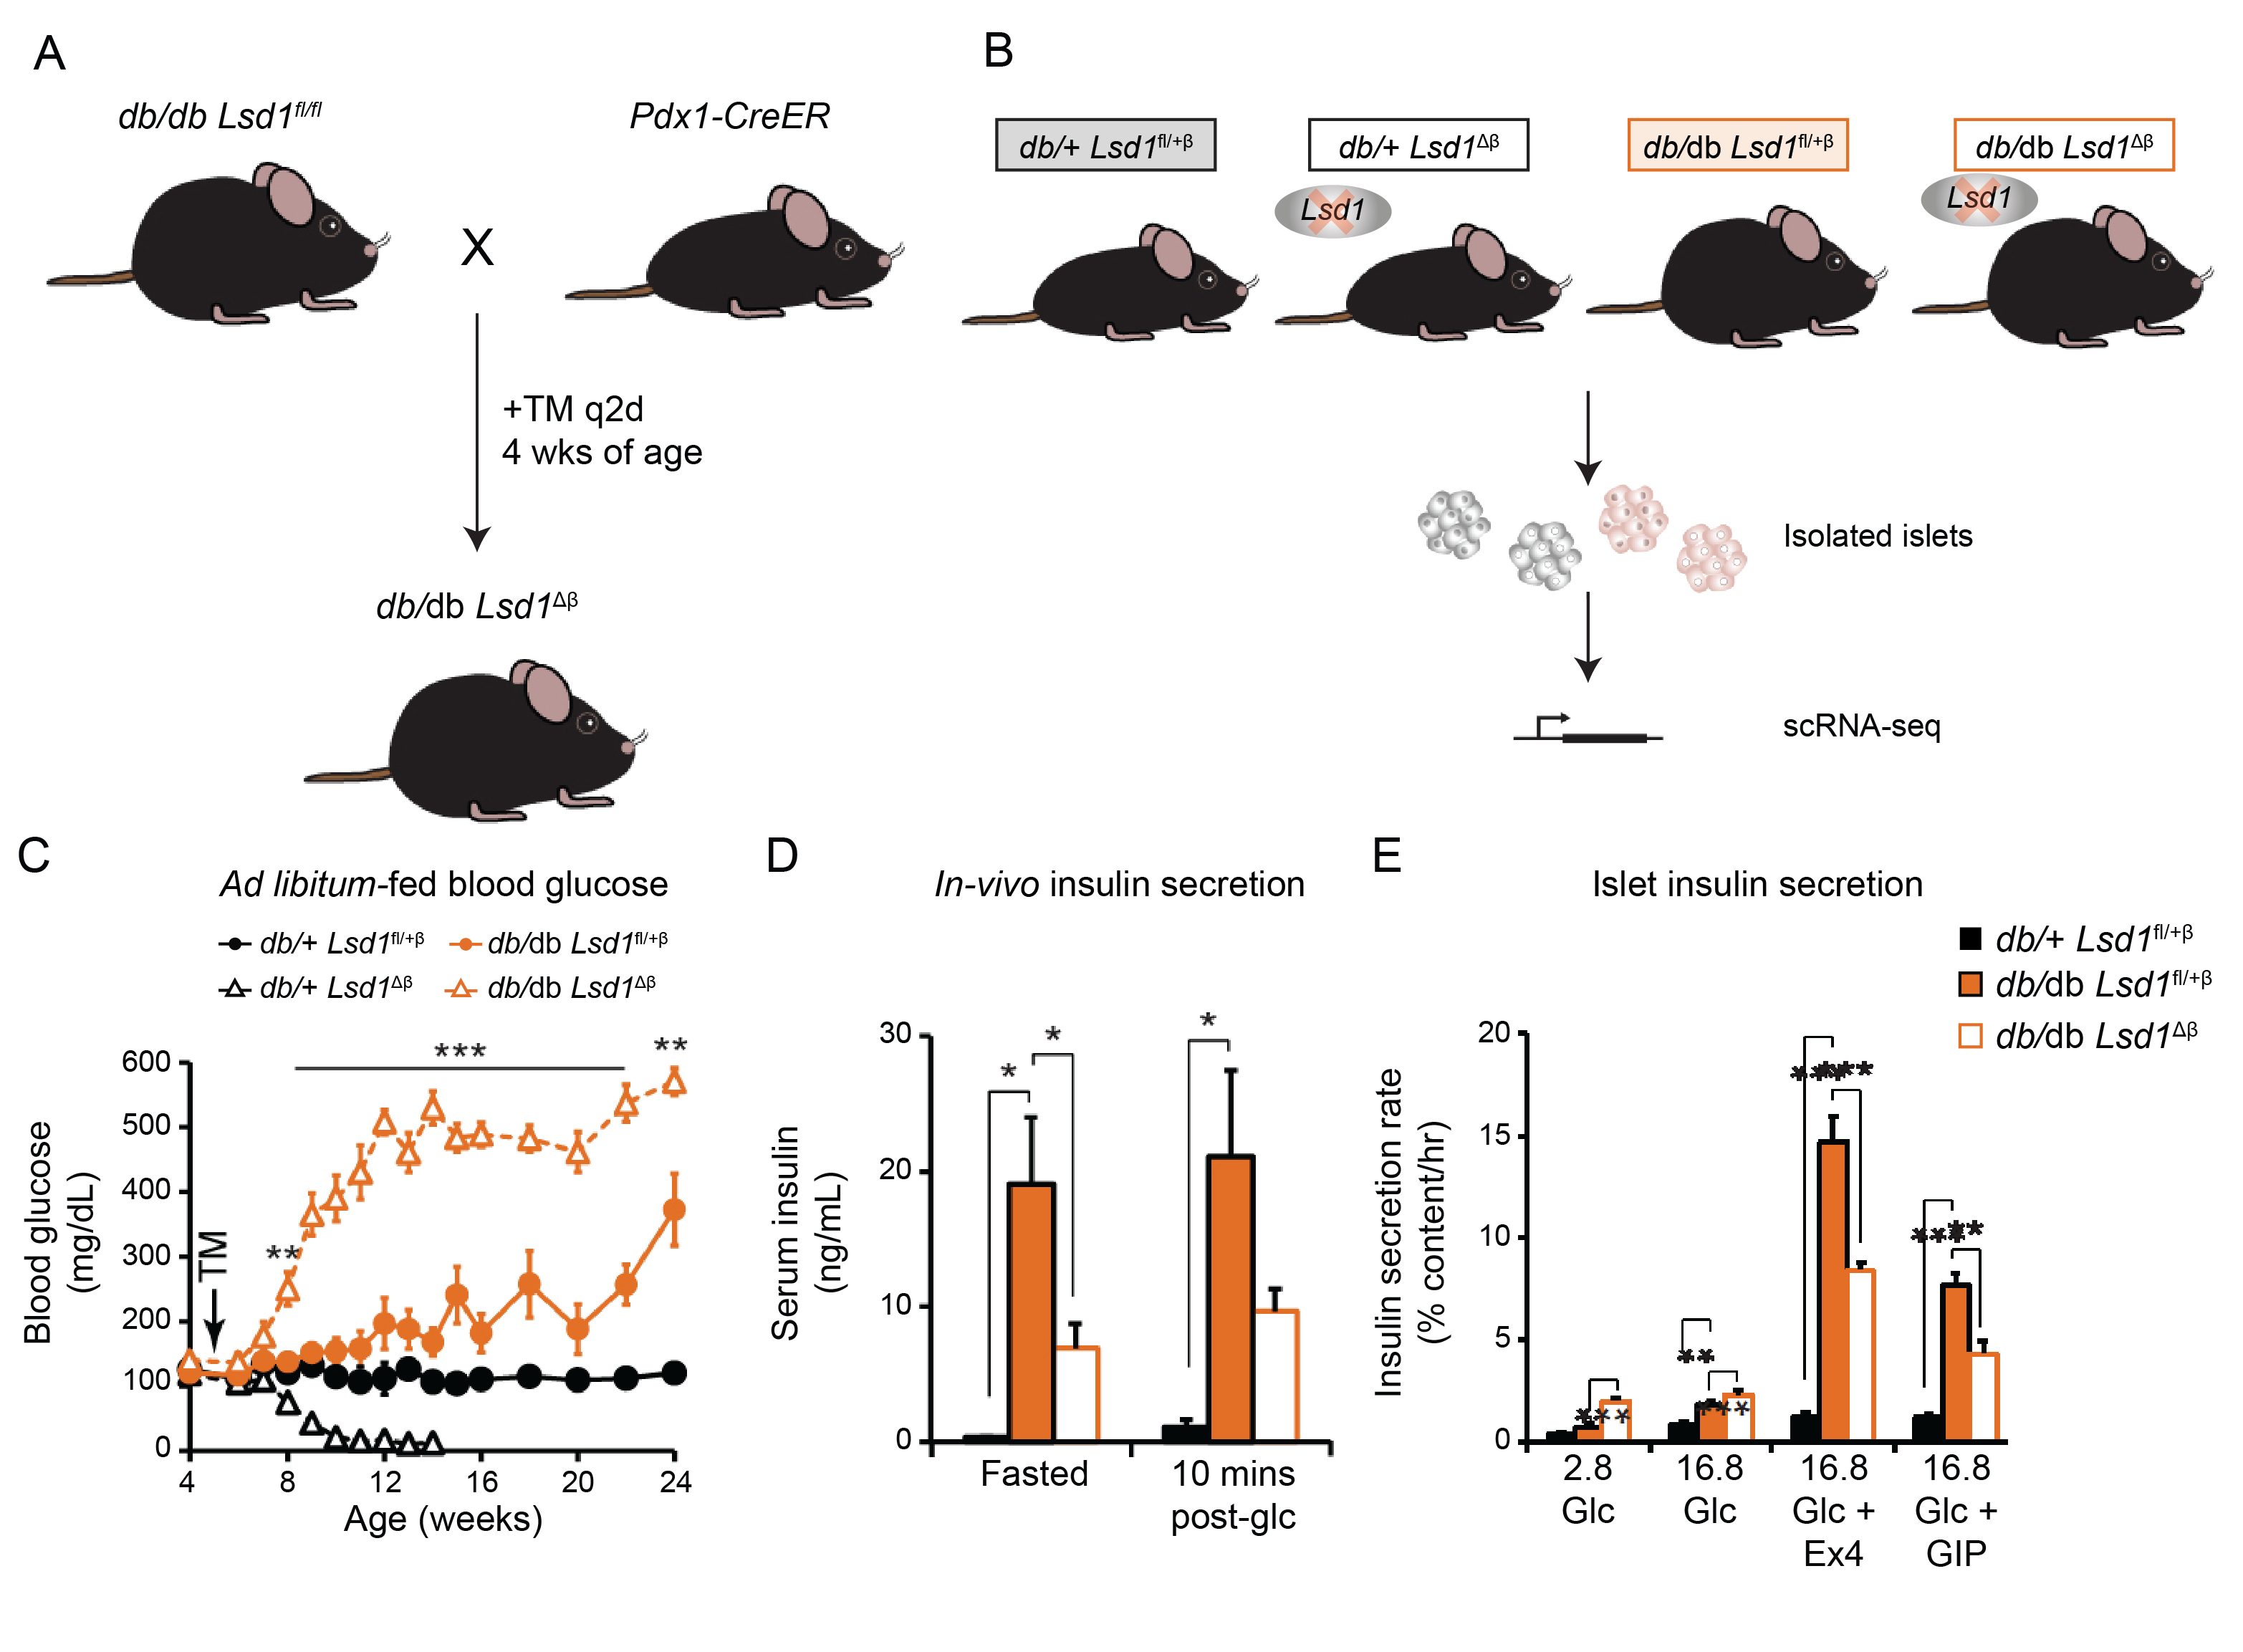
\includegraphics[width=\linewidth]{Chapter5/Fig/F3-20-01.png}
    \caption[Functional characterization of \textit{Lsd1} inactivation]{\textbf{Functional characterization of \textit{Lsd1} inactivation.} \textbf{(A)} Blood glucose levels in ad libitum-fed lean and obese mice with or without \textit{Lsd1} deletion. \textit{n} = 5-10 mice. \textbf{(B)} Serum insulin levels in 9-week-old lean and obese mice with or without \textit{Lsd1} deletion, measured under fasting conditions and 10 minutes post glucose administration. \textit{n} = 4-6 mice. \textbf{(C)} Insulin secretion assay in isolated islets from 9-week-old lean and obese mice with or without \textit{Lsd1} deletion, stimulated with indicated glucose (glc) concentrations (in mM) and with Exendin-4 (Ex-4) and \acrfull{gip}. \textit{n} = 6-12 islets. All statistical comparisons were made with unpaired, 2-tailed \textit{t} test. $\textsuperscript{*} p < 0.05, \textsuperscript{**} p < 0.01, \textsuperscript{***} p < 0.001$. Abbreviations: TM, tamoxifen. \textit{This figure was originally generated by Dr. Matthew Wortham and has been adapted here with permission.}}
    \label{fig:chp3_valid_study_metab}
\end{figure}

-- underlies the acceleration of hyperglycemia observed in this model \textbf{(\autoref{fig:chp3_valid_study_metab} C)}. Overall, \textit{Lsd1} seemed to have distinct effects on systemic glucose metabolism in lean and obese states.




%Insulin secretion assays

\subsubsection{\large Scoring of gene modules identified from pseudobulk $\beta$-cells}

\par To identify functional processes that are characteristic of the $\beta$-cells obtained from the islets of lean and obese mice with or without intact \textit{Lsd1}, we performed gene set scoring of the modules identified from the pseudobulk $\beta$-cells across all samples \textbf{(\autoref{fig:chp3_valid_study_genescores};} see \textbf{\hyperref[subsubsec:met_chp3_scoring]{Methods})}. The Workload-repressed module was highly expressed in lean mice with \textit{Lsd1} intact \textbf{(\autoref{fig:chp3_valid_study_genescores} A)}. This module consisted of genes related to mature $\beta$-cell identity and $\beta$-cell functional identity. This was also observed in the case of the older 9-week-old animals, wherein the module was further up-regulated compared to the younger mice. The overall expression of this module progressively declined in lean mice when \textit{Lsd1} was deleted, followed by obese animals with \textit{Lsd1} intact and \textit{Lsd1} deleted, in which the module was least expressed \textbf{(\autoref{fig:chp3_valid_study_genescores} A)}. Interestingly, the 9-week-old obese mice with \textit{Lsd1} deletion scored higher for this module in comparison to their 6-week-old counterparts. This could likely be due to the additive nature of \textit{db/db} and \textit{Lsd1} effects, which work to enhance insulin secretion, resulting in up-regulation of secretion machinery, but at the cost of later defects.\\


\par The Workload-activated and Decompensation modules associated in an opposite manner to that of Workload-repressed module \textbf{(\autoref{fig:chp3_valid_study_genescores} B,C)}. The obese \textit{db/db} mice with \textit{Lsd1} deletion showed a higher up-regulation of the genes in these modules, with the 9-week-old animals exhibiting a stronger trend than the 6-week-old animals \textbf{(\autoref{fig:chp3_valid_study_genescores} B,C)}. The $\beta$-cells in the obese 9-week-old mice are likely decompensated against the 

\begin{figure}[H]
    \centering
    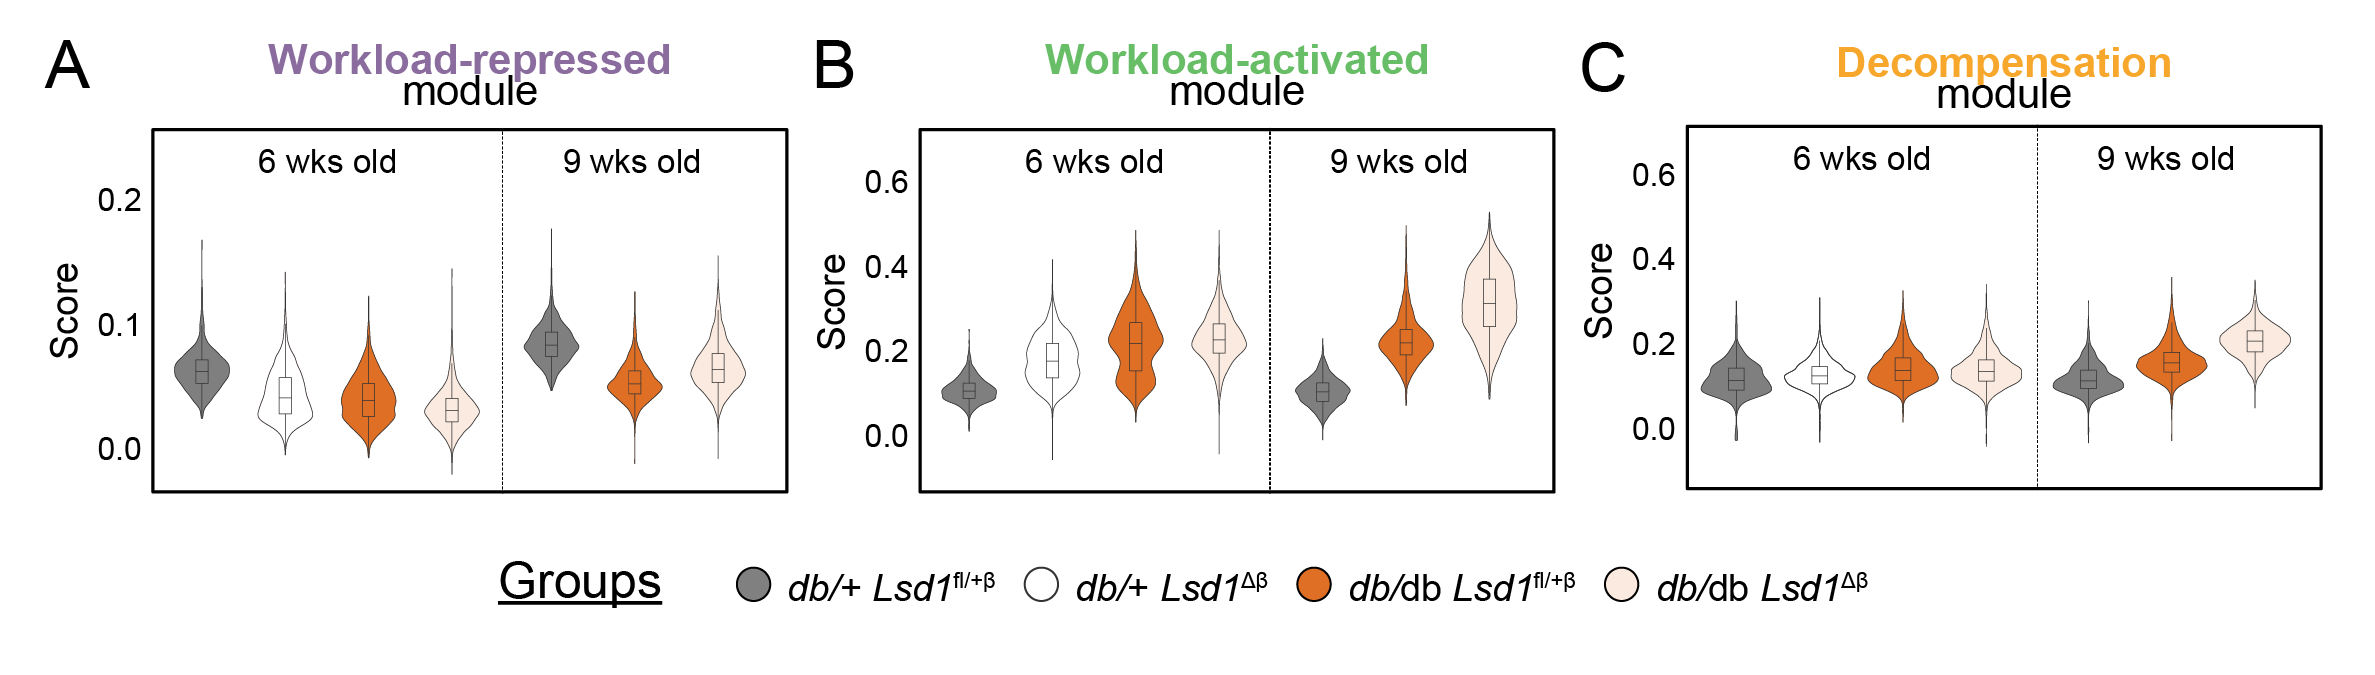
\includegraphics[width=\linewidth]{Chapter5/Fig/F3-17-01.png}
    \caption[Activity of workload-associated gene modules in the external study]{\textbf{Activity of workload-associated gene modules due to overworking $\beta$-cells through \textit{Lsd1} inactivation during obesity.} \textbf{(A) - (C)} Violin plots depicting the gene set score for Workload-repressed module \textbf{(A)}, Workload-activated module \textbf{(B)} and Decompensation module \textbf{(C)} in the 6-week-old and 9-week-old animals for all experimental groups in the external study. For all violin plots,on the overlay box plots, the middle horizontal line represents the median, the box represents the inter-quartile range and the whiskers represent the minimum and maximum values.}
    \label{fig:chp3_valid_study_genescores}
\end{figure}

hyperglycemic environment, in addition to up-regulation of insulin secretion due to \textit{Lsd1} deletion, the combined effects of which cause the $\beta$-cell to eventually fail.

\subsubsection{\large Query mapping and transfer of annotations}

Next, we mapped our annotated $\beta$-cell subset from the integrated atlas onto the $\beta$-cells from this external study \textbf{(\autoref{fig:chp3_valid_study_composition};} see \hyperref[subsubsec:met_chp3_validation]{\textbf{Methods}}\textbf{)}. This allowed us to better understand the compositional shifts of the identified $\beta$-cell subsets in the integrated atlas during compensatory mechanisms in response to insulin resistance during obesity. The 6-week-old and 9-week-old lean animals with intact \textit{Lsd1} (\textit{db/+ Lsd1\textsuperscript{fl/+$\beta$}}) exhibited a composition of $\beta$-1 normal and $\beta$-2 compensating subsets similar to the controls of the meta-analysis \textbf{(\autoref{fig:chp3_valid_study_composition})}. Next, we observed the progressive enrichment of $\beta$-2 compensating subset in the 6-week-old animals - with \textit{Lsd1} deletion in the lean mice (\textit{db/+ Lsd1\textsuperscript{$\Delta\beta$}}), \textit{Lsd1} intact in the obese \textit{db/db} animals (\textit{db/db Lsd1\textsuperscript{fl/+$\beta$}})  and with \textit{Lsd1} deletion in \textit{db/db} animals (\textit{db/+ Lsd1\textsuperscript{$\Delta\beta$}})  which were primarily composed of the compensating subset. Through this mapping procedure, we also identified increased abundance of the $\beta$-3 stress-immature subset in the older 9-week-old \textit{db/db} animals with \textit{Lsd1} deletion (\textit{db/db Lsd1\textsuperscript{$\Delta\beta$}}). Interestingly, the same genotype in the 6-week-old animals were primarily composed of the $\beta$-2 compensating subset. This likely suggests a shift from the compensating state in the 6-week-old mice to a stressed-immature and decompensated state in the 9-week-old mice, and that the $\beta$-2 compensating and the  


\begin{figure}[H]
    \centering
    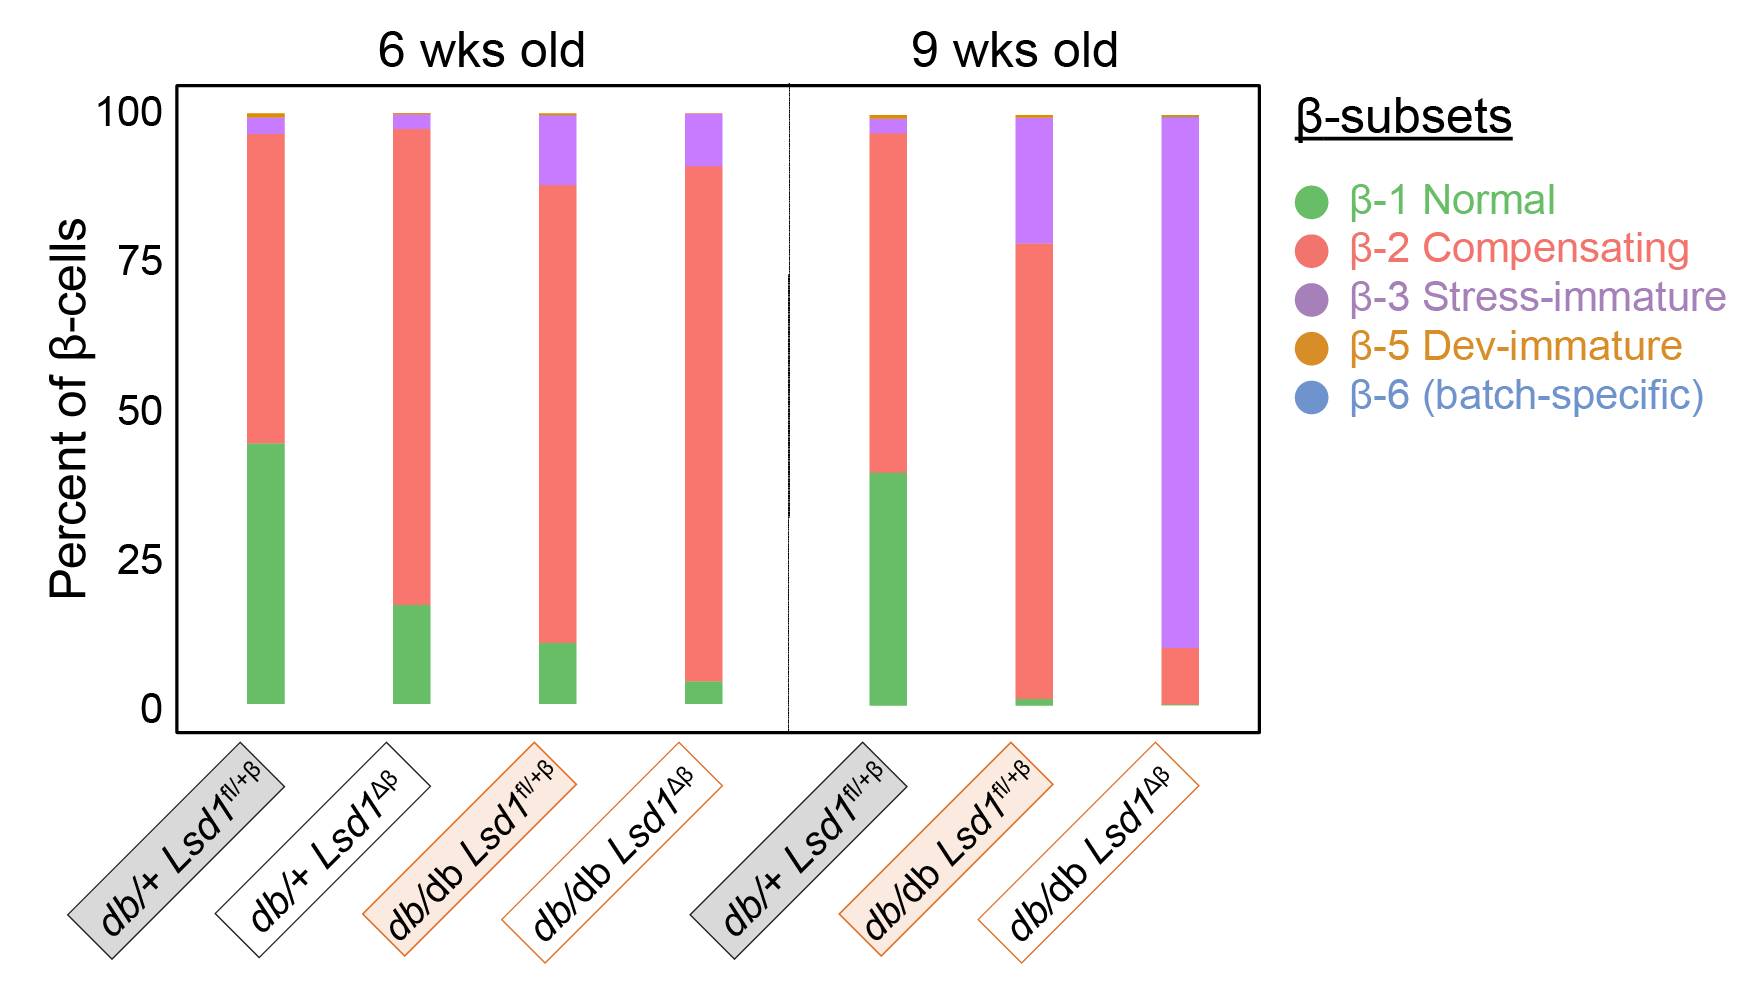
\includegraphics[width=\linewidth]{Chapter5/Fig/F3-17-03.png}
    \caption[Composition shifts of $\beta$-cell subsets in external study]{\textbf{Composition shifts of $\beta$-cell subsets in external study.} Bar plots depicting the composition of the experimental groups for two time-points in the external study, across the transferred $\beta$-cell subset annotations from the integrated atlas. The compositions were computed as percentage of cells in each subset over all cells in the group.}
    \label{fig:chp3_valid_study_composition}
\end{figure}

$\beta$-3 stress-immature cells also represent different states along the axis of $\beta$-cell adaptation and decompensation.\\




% This composition distribution was more similar to what was observed for the lean animals in the mild genetic obesity study included in the integrated analysis \textbf{(\autoref{fig:chp3_betasubsets} D)} that \textit{Lsd1} deletion serves to


In summary, overworking $\beta$-cells through \textit{Lsd1} inactivation during obesity in younger animals resulted in progressive enrichment of the compensating subset at the expense of normal $\beta$-cells. The near total depletion of the normal $\beta$-cells in the older \textit{db/db} islets with or without \textit{Lsd1} suggests the acceleration of normal disease progression with the enrichment of the compensating and the stress-immature subsets. These subset composition shifts are correlated with the up-regulation of genes involved in increased $\beta$-cell workload and decompensation. It is likely that the subset composition shifts observed at earlier stages simply predispose $\beta$-cells to dysfunction and failure, with the compensating phenotype being vulnerable to any subsequent stressors.

\clearpage

\section[Summary]{Summary}
\label{sec:chp3_summary}

\par In our study, we have generated an integrated single-cell transcriptomic atlas of $\beta$-cells, utilizing both in-house generated and publicly available \gls{scr} datasets, to elucidate mechanisms underlying $\beta$-cell compensatory responses under varying workload conditions. Following rigorous \gls{qc} and preprocessing workflow, we minimized batch effects and re-annotated cell types independent of the original study annotations.\\

\par We assessed an integrated $\beta$-cell subset and revealed that transcriptional responses activated and repressed in response to increased workload and hyperglycemia are largely consistent across various models. In addition, severe hyperglycemic models that induced $\beta$-cell decompensation resulted in the activation of decompensatory-specific transcriptional signatures. Notably, these adaptations reflect the key molecular changes observed in human \gls{t2d}, including the down-regulation of genes essential to $\beta$-cell identity and the up-regulation of stress response pathways.\\

\par Furthermore, we characterized $\beta$-cell heterogeneity and identified three major $\beta$-cell subsets:

\begin{enumerate}
    \item \textbf{$\beta$-1 normal:} exhibited expression of markers related to $\beta$-cell maturity and function and is the predominant subset in unchallenged controls and the old 2-year-old mice, indicating a stable, functional state.
    \item \textbf{$\beta$-2 compensating:} showed enrichment of genes related to \gls{er}-resident protein folding machinery and exhibited universal enrichment across all models of adaptation and decompensation, except partial $\beta$-cell ablation, thereby suggesting an adaptive response to maintain cellular homeostasis under stress.
    \item \textbf{$\beta$-3 stress-immature:} characterized by established markers of $\beta$-cell immaturity (\textit{e.g. Cd81}) and a dedifferentiation profile, reflecting $\beta$-cell functional impairment under severe hyperglycemic conditions.
\end{enumerate}

By ordering $\beta$-cells along an axis of maturity and workload, we delineated the gradual shift from normal to compensating states under increased workloads and the accelerated switch to the stress-immature state under severe hyperglycemic conditions. We also demonstrated the usability our $\beta$-cell transcriptome atlas by mapping additional \gls{scr} datasets onto the atlas, therefore gaining additional insights on the progressive nature of $\beta$-cell dysfunction under diabetic conditions. These comparative analysis set up a framework for future single-cell transcriptomics studies on $\beta$-cell workload to be incorporated into our reference atlas and thereby improving the scope, quality and robustness of this resource overall.\\

Overall, our comprehensive study not only enhances the understanding of $\beta$-cell functionality and adaptation under various stress, but also provides a valuable resource to the field of islet biology and \gls{t2d} research.

%\newpage\null\thispagestyle{empty}\newpage